% Gelfand seminar notes, 1978-79: source pages P000786-P000825, P000829-P000842.
% English translation (AI-made, checked against the scans), cut page by page from the cumulative working reader A4-reader-chapters01-34-complete-first1527-separated-diplomatic-r42.
% \SourcePage{GELFAND-Pnnnnnn}{label} starts a scanned page; the second argument is the number written
% on the page, if any. Editorial notes give the page, a label and the transcriber's remark; \Unclear
% marks a doubtful reading.
\SourcePage{GELFAND-P000786}{4}

\underline{30.10.78.}\qquad\underline{Gelfand Seminar}
\Unclear{GELFAND-P000786}{heading-date}{The month looks more like 10. A break in the second digit leaves 11 possible.}
\end{GelfandAdjacentEvidence}
\begin{GelfandAdjacentEvidence}{GELFAND-P000786}{2}


\underline{Kruskal}

\underline{Surreal numbers}

there are 2 books:
\underline{John Conway} --- (“combinatorial games”).

\(\{\)\underline{Knuth} D. “[crossed out: \ldots{}] --- novel”\(\}\)
\Incomplete{GELFAND-P000786}{book-cancellation}{Dense hatching obscures the entry before “--- novel”.}
\end{GelfandAdjacentEvidence}
\begin{GelfandAdjacentEvidence}{GELFAND-P000786}{3}


\uuline{Def.}

\underline{Number} \(=\) \uwave{map from a well-ordered set to a set of 2 elements} \(\uparrow\) and \(\downarrow\).
\Incomplete{GELFAND-P000786}{definition-bar}{A heavily inked horizontal mark lies below the wavy line. No letters can be distinguished.}
\end{GelfandAdjacentEvidence}
\begin{GelfandAdjacentEvidence}{GELFAND-P000786}{4}


\(x\ne y\) --- compare the arrows (lexicographically).
\[
\widehat{\uparrow}=\uparrow\uparrow\uparrow\ldots=\omega
\]
\(\widehat{\phantom{x}}\leftrightarrow\) (periodic)

\(\widehat{\uparrow\downarrow}\qquad\widehat{\downarrow}\)

\SourceFigure{GELFAND-P000786}{number-line}{%
\par\begingroup\color{black}\GelfandFitDiagram{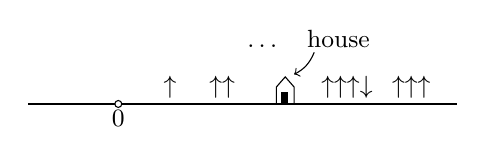
\begin{tikzpicture}[x=.80cm,y=.80cm,every node/.style={font=\small,inner sep=1pt}]
\draw (0,0)--(6.8,0);
\draw[fill=white] (1.43,0) circle (.055);
\node[below] at (1.43,-.05) {\(0\)};
\node[above] at (2.25,.04) {\(\uparrow\)};
\node[above] at (3.08,.04) {\(\uparrow\uparrow\)};
\draw (3.94,0)--(3.94,.27)--(4.08,.43)--(4.22,.27)--(4.22,0)--cycle;
\fill (4.02,0) rectangle (4.13,.19);
\draw[->] (4.54,.82) to[bend left=20] (4.22,.47);
\node at (4.45,1.03) {\sout{\ldots}\quad house};
\node[above] at (5.06,.04) {\(\uparrow\uparrow\uparrow\downarrow\)};
\node[above] at (6.08,.04) {\(\uparrow\uparrow\uparrow\)};
\end{tikzpicture}}\endgroup
\par The crossed-out word before “house” is illegible.}
\end{GelfandAdjacentEvidence}
\begin{GelfandAdjacentEvidence}{GELFAND-P000786}{5}


\SourceFigure{GELFAND-P000786}{binary-tree}{%
\par\begingroup\color{black}\GelfandFitDiagram{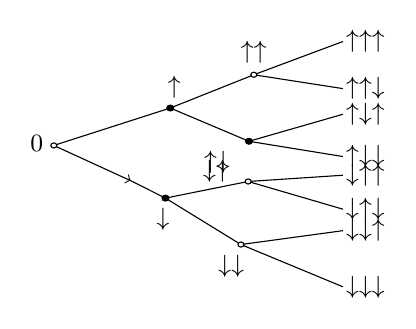
\begin{tikzpicture}[x=1.02cm,y=.88cm,every node/.style={font=\small,inner sep=1pt}]
\coordinate (O) at (0,0);
\coordinate (U) at (1.45,.54);
\coordinate (D) at (1.39,-.76);
\coordinate (UU) at (2.49,1.02);
\coordinate (UD) at (2.43,.06);
\coordinate (DU) at (2.42,-.52);
\coordinate (DD) at (2.33,-1.43);
\draw (O)--(U)--(UU)--(3.60,1.50) node[right] {\(\uparrow\uparrow\uparrow\)};
\draw (UU)--(3.60,.82) node[right] {\(\uparrow\uparrow\downarrow\)};
\draw (U)--(UD)--(3.60,.45) node[right] {\(\uparrow\downarrow\uparrow\)};
\draw (UD)--(3.60,-.16) node[right] {\(\uparrow\downarrow\downarrow\)};
\draw[->] (O)--(.96,-.51);
\draw (.96,-.51)--(D)--(DU)--(3.60,-.43) node[right] {\(\downarrow\uparrow\uparrow\)};
\draw (DU)--(3.60,-.92) node[right] {\(\downarrow\uparrow\downarrow\)};
\draw (D)--(DD)--(3.60,-1.23) node[right] {\(\downarrow\downarrow\uparrow\)};
\draw (DD)--(3.60,-2.04) node[right] {\(\downarrow\downarrow\downarrow\)};
\foreach \vertex in {O,UU,DU,DD}{\draw[fill=white] (\vertex) circle (.037);}
\foreach \vertex in {U,UD,D}{\fill (\vertex) circle (.051);}
\node[left] at (-.09,.03) {\(0\)};
\node[above] at (1.50,.63) {\(\uparrow\)};
\node[above] at (2.49,1.13) {\(\uparrow\uparrow\)};
\node[below] at (2.03,-.03) {\(\uparrow\downarrow\)};
\node[below] at (1.36,-.86) {\(\downarrow\)};
\node[above] at (2.02,-.58) {\(\downarrow\uparrow\)};
\node[below] at (2.21,-1.54) {\(\downarrow\downarrow\)};
\end{tikzpicture}}\endgroup}
\end{GelfandAdjacentEvidence}
\begin{GelfandAdjacentEvidence}{GELFAND-P000786}{6}


\(\ldots\}\,=\,\ldots\)
\Incomplete{GELFAND-P000786}{faint-formula-right}{A right brace and an equals sign are visible under the number line. The other faint strokes do not establish the expression.}
\end{GelfandAdjacentEvidence}


\[
x\underset{\substack{\vert\\\text{earlier}\\\text{(earlier)}}}{\longleftarrow}y
\]
(i.e. \(x\) is on the path from \(0\) to \(y\))

\(y]\) --- an element of the set of numbers that come before \(y\)

\uwave{Truncation operation} --- \(x\) has fewer arrows

\(y\rceil\) a number earlier than \(y\), but greater than it

\(y\rfloor\) ---\,\textquotedblleft\,--- and less than it

\(x<y\) is also defined
\begin{gather*}
\{y]\}=\{y\rfloor\}\cup\{y\rceil\},\\
\{y\rceil\}\cap\{y\rfloor\}=\Lambda
\end{gather*}

\underline{Example:}

\uwave{Main def.:}


\Needspace{7\baselineskip}
\begin{GelfandAdjacentEvidence}{GELFAND-P000787}{1}
\SourcePage{GELFAND-P000787}{unlabelled}

\underline{Thm. 1}

(simple)

\(A,B\) --- \uwave{sets of numbers}

\(\forall a\in A,b\in B\); [crossed out: \ldots{}] \(a<b\)
\Unclear{GELFAND-P000787}{theorem-one-cancellation}{A heavily crossed-out sign lies between the semicolon and the inequality.}
\end{GelfandAdjacentEvidence}
\begin{GelfandAdjacentEvidence}{GELFAND-P000787}{2}


\uwave{Then} \(\exists x:\quad a<x<b.\)

\uwave{and there exists a unique earliest} \(\underline{x}\).

\underline{Proof:} transfinite ind., we look at \(x=0\) and if we have not found \(x\) up to a certain point, we look further.

\underline{Notation:}

\SourceFigure{GELFAND-P000787}{looped-braces}{%
\par\begingroup\color{black}\GelfandFitDiagram{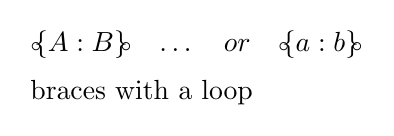
\begin{tikzpicture}[every node/.style={inner sep=1pt}]
\node (notation) {\(\displaystyle \mathopen{{\scriptstyle\circ}\mkern-5mu\{} A:B \mathclose{\}\mkern-5mu{\scriptstyle\circ}}\quad\text{\sout{…}}\quad
  \text{or}\quad \mathopen{{\scriptstyle\circ}\mkern-5mu\{} a:b \mathclose{\}\mkern-5mu{\scriptstyle\circ}}\)};
\node[anchor=north west] at ([yshift=-2mm]notation.south west) {braces with a loop};
\end{tikzpicture}}\endgroup}
\end{GelfandAdjacentEvidence}
\begin{GelfandAdjacentEvidence}{GELFAND-P000787}{3}

\Unclear{GELFAND-P000787}{notation-cancellation}{The cancelled sign before “or” resembles Russian «и» (“and”).}
\end{GelfandAdjacentEvidence}
\begin{GelfandAdjacentEvidence}{GELFAND-P000787}{4}


\underline{Addition.}

by transfinite induction.

\underline{Theorem 2}
\[
x=\mathopen{{\scriptstyle\circ}\mkern-5mu\{} x\rfloor:x\rceil \mathclose{\}\mkern-5mu{\scriptstyle\circ}}
\]
(obvious)

\underline{Def. of addition.}
\[
x+y=\mathopen{{\scriptstyle\circ}\mkern-5mu\{} x\rfloor+y,\ x+y\rfloor:\ x\rceil+y,\ x+y\rceil \mathclose{\}\mkern-5mu{\scriptstyle\circ}}
\]

\underline{Theorem 3.}

a) \(0+0=\mathopen{{\scriptstyle\circ}\mkern-5mu\{} : \mathclose{\}\mkern-5mu{\scriptstyle\circ}}=0.\)

[Below the formula:] there are no conditions, so the earliest of all

b) [crossed out: \ldots{}] \(x+0=x\) by induction
\Unclear{GELFAND-P000787}{zero-quantifier-cancellation}{The cancelled strokes resemble \(\forall x\).}
\end{GelfandAdjacentEvidence}
\begin{GelfandAdjacentEvidence}{GELFAND-P000787}{5}


\underline{Proof:}
\SourceFigure{GELFAND-P000787}{induction-pointer}{%
\par\begingroup\color{black}\GelfandFitDiagram{\begin{tikzpicture}[every node/.style={inner sep=1pt}]
\node {\(\displaystyle
\begin{aligned}
x+0&=\mathopen{{\scriptstyle\circ}\mkern-5mu\{} x\rfloor+0:x\rceil+0 \mathclose{\}\mkern-5mu{\scriptstyle\circ}}\\
&\underset{\text{ind.}}{=}\mathopen{{\scriptstyle\circ}\mkern-5mu\{} x\rfloor:x\rceil \mathclose{\}\mkern-5mu{\scriptstyle\circ}}
\underset{\substack{\nearrow\\\text{Thm. 2.}}}{=}x
\end{aligned}\)};
\end{tikzpicture}}\endgroup}
\end{GelfandAdjacentEvidence}
\begin{GelfandAdjacentEvidence}{GELFAND-P000787}{6}


In the ordinary theory there is no notion of earlier!

\(x+y\) --- the simplest number, monotone in each argument

a) monotone in \(x,y\)

b) the earliest of all such numbers.

The usual properties hold
\begin{gather*}
x+y=y+x\\
(x+y)+z=x+(y\mathbin{\text{[?]}}z)
\end{gather*}
\Unclear{GELFAND-P000787}{associativity-sign}{The sign between \(y\) and \(z\) resembles \(\ge\). The reading \(+\) is also possible.}
\end{GelfandAdjacentEvidence}


\uwave{There is an inverse operation.}

The opposite of \(x\) --- reversal of the arrows\qquad
\(x+\operatorname{opp}.x=0\).


\Needspace{7\baselineskip}
\begin{GelfandAdjacentEvidence}{GELFAND-P000788}{1}
\SourcePage{GELFAND-P000788}{5}
\[
\uparrow+\uparrow=\mathopen{{\scriptstyle\circ}\mkern-5mu\{}1,1:\Lambda\}=\uparrow\uparrow
\]
\Unclear{GELFAND-P000788}{top-sum}{The initial signs on either side of the plus resemble up arrows. “1+1” is also a possible reading. The ones within the braces have feet.}
\end{GelfandAdjacentEvidence}
\begin{GelfandAdjacentEvidence}{GELFAND-P000788}{2}


\underline{\underline{Ex.}}
\begin{gather*}
\uparrow\downarrow+\uparrow\downarrow=?\\
\widehat{\uparrow}+\downarrow\downarrow\downarrow=?
\end{gather*}

\underline{Multiplication.}

\underline{Basic inequality} of \underline{mult'n.}

\[
r<s,\qquad u<v
\]
\Unclear{GELFAND-P000788}{basic-letter}{The sign before \(<s\) is provisionally typeset as \(r\). Its shape also admits \(\eta\).}
\end{GelfandAdjacentEvidence}
\begin{GelfandAdjacentEvidence}{GELFAND-P000788}{3}


Then
\[
ru+sv\mathrel{\text{[?]}}rv+su
\]
\Unclear{GELFAND-P000788}{basic-products}{The first letters in \(ru\) and \(rv\) have been retraced. The sign after \(sv\) is overwritten and resembles \(>\).}
\end{GelfandAdjacentEvidence}
\begin{GelfandAdjacentEvidence}{GELFAND-P000788}{4}


\(xy\) --- any of the four \textup{[?]}\ \(\Rightarrow\) 4 inequalities
\Unclear{GELFAND-P000788}{four-products-word}{The abbreviation after “four” may be «слаг.» (summands) or «оп.» (options).}
\end{GelfandAdjacentEvidence}
\begin{GelfandAdjacentEvidence}{GELFAND-P000788}{5}


\[
\begin{aligned}
x\cdot y={}&\mathopen{{\scriptstyle\circ}\mkern-5mu\{}x\rfloor\cdot y+x\cdot y\rfloor-x\rfloor\cdot y\rfloor,\\
&\phantom{\{}x\rceil\cdot y+x\cdot y\rceil-x\rceil\cdot y\rceil:\\
&\phantom{\{}x\rfloor\cdot y+x\cdot y\rceil-x\rfloor\cdot y\rceil,\\
&\phantom{\{}x\rceil\cdot y+x\cdot y\rfloor-x\rceil\cdot y\rfloor\}
\end{aligned}
\]
\Unclear{GELFAND-P000788}{recursion-mark}{A heavy cross-shaped mark stands above the comma at the end of the third line. Its purpose is unclear.}
\end{GelfandAdjacentEvidence}
\begin{GelfandAdjacentEvidence}{GELFAND-P000788}{6}


The natural properties of multiplication hold.
\[
x\cdot0=\mathopen{{\scriptstyle\circ}\mkern-5mu\{}:\mathclose{\}\mkern-5mu{\scriptstyle\circ}}=0,\qquad x\cdot1=x
\]
\[
\begin{aligned}
x\cdot1&=\mathopen{{\scriptstyle\circ}\mkern-5mu\{}x\rfloor\cdot1+x\cdot0-x\rfloor\cdot0:\\
&\qquad x\rceil\cdot1+x\cdot0-x\rceil\cdot0\mathclose{\}\mkern-5mu{\scriptstyle\circ}}\\
&=\mathopen{{\scriptstyle\circ}\mkern-5mu\{}x\rfloor+0-0:x\rceil+0-0\mathclose{\}\mkern-5mu{\scriptstyle\circ}}=x
\end{aligned}
\]

Associat., commut., distribut. hold.

\uwave{Prove at home.}

\underline{\underline{Advice.}} Technical device.

Prove that the def. [crossed out: \sout{?}] [inserted above the line with a caret:] of addition is “indifferent to brackets”

\hfill\uwave{bracket indifferent}

\Unclear{GELFAND-P000788}{advice-cancellation}{The heavily crossed-out abbreviation may read «умн.» (mult.).}
\end{GelfandAdjacentEvidence}


\begin{gather*}
x=\mathopen{{\scriptstyle\circ}\mkern-5mu\{}a:b\mathclose{\}\mkern-5mu{\scriptstyle\circ}}\\
y=\mathopen{{\scriptstyle\circ}\mkern-5mu\{}c:d\mathclose{\}\mkern-5mu{\scriptstyle\circ}}\\
x+y=\mathopen{{\scriptstyle\circ}\mkern-5mu\{}a+y,x+c:b+y,x+d\mathclose{\}\mkern-5mu{\scriptstyle\circ}}
\end{gather*}

Multiplication also has this property.

\uwave{Associat.}

There exist inf. large and inf. small numbers.


\Needspace{7\baselineskip}
\begin{GelfandAdjacentEvidence}{GELFAND-P000789}{1}
\SourcePage{GELFAND-P000789}{unlabelled}
\[
\uparrow\uparrow\uparrow\ldots=\widehat{\uparrow}=\omega
\quad\text{--- the simplest inf. number.}
\]
\Unclear{GELFAND-P000789}{top-infinite-abbreviation}{The abbreviation before «число» (“number”) provisionally reads «беск.» (inf.).}
\end{GelfandAdjacentEvidence}
\begin{GelfandAdjacentEvidence}{GELFAND-P000789}{2}


\[
\uparrow\downarrow\downarrow\ldots=\uparrow\widehat{\downarrow}=\varepsilon
\]

\SourceFigure{GELFAND-P000789}{nested-dyadic-brackets}{%
\par\begingroup\color{black}\GelfandFitDiagram{\begin{tikzpicture}[x=1cm,y=1cm,every node/.style={inner sep=1pt}]
\node at (.26,2.16) {\(1\)};
\draw (.06,1.87)--(.04,1.72)--(1.10,1.75) to[out=0,in=-75] (1.18,1.87);
\node at (.57,1.35) {\(\tfrac12\)};
\draw (0,1.18)--(-.02,.92)--(2.03,1.07) to[out=8,in=-77] (2.12,1.23);
\node at (1.20,.63) {\(1/4\)};
\end{tikzpicture}}\endgroup}
\end{GelfandAdjacentEvidence}
\begin{GelfandAdjacentEvidence}{GELFAND-P000789}{3}


\begin{gather*}
\omega\cdot\varepsilon=1\\
\omega+\varepsilon=\widehat{\uparrow}\uparrow\widehat{\downarrow}
\end{gather*}

Sometimes one can shorten it, but sometimes one cannot.

\uwave{Ordinal arithmetic.}

[crossed out: \sout{\ldots}] [inserted above:] ordinals: numbers with arrows \(\uparrow\) (without arrows \(\downarrow\)).
\Incomplete{GELFAND-P000789}{ordinals-cancellation}{The word below the insertion “ordinals” is heavily crossed out and illegible.}
\end{GelfandAdjacentEvidence}
\begin{GelfandAdjacentEvidence}{GELFAND-P000789}{4}


The arithmetic is different from the ordinary one!

The ordinary one is not commutative!

\SourceFigure{GELFAND-P000789}{ordinal-addition}{%
\par\begingroup\color{black}\GelfandFitDiagram{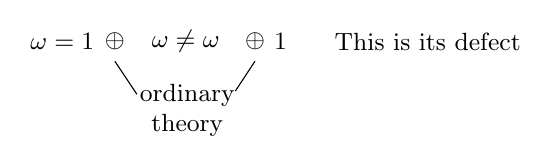
\begin{tikzpicture}[x=1cm,y=1cm,every node/.style={font=\small,inner sep=1pt}]
\node[anchor=east] at (.77,0) {\(\omega=1\)};
\node at (.99,0) {\(\oplus\)};
\node at (1.89,0) {\(\omega\ne\omega\)};
\node at (2.77,0) {\(\oplus\)};
\node[anchor=west] at (2.97,0) {\(1\)};
\node[anchor=west] at (3.74,0) {This is its defect};
\draw (.99,-.25)--(1.27,-.67);
\draw (2.77,-.25)--(2.52,-.63);
\node[align=center] at (1.91,-.87) {ordinary\\theory};
\end{tikzpicture}}\endgroup}
\end{GelfandAdjacentEvidence}
\begin{GelfandAdjacentEvidence}{GELFAND-P000789}{5}


Hessenburg devis. a natural def. of add. and mult. of transfin. numbers.
\Unclear{GELFAND-P000789}{hessenburg-spelling}{The last letters of the surname provisionally read “burg”.}
\end{GelfandAdjacentEvidence}
\begin{GelfandAdjacentEvidence}{GELFAND-P000789}{6}

\Unclear{GELFAND-P000789}{hessenburg-definition-abbreviation}{The abbreviation after the name provisionally reads «прид.» (devis.).}
\end{GelfandAdjacentEvidence}
\begin{GelfandAdjacentEvidence}{GELFAND-P000789}{7}


It turned out that it coincid. with this one

\(\forall\) number, except \(0\), has an inverse \(\frac1x\), \(x\ne0\).

\(\frac yx\) exists

\underline{\(\forall x>0\) there is \(\sqrt{x}\)} --- by inf. ind.
\Unclear{GELFAND-P000789}{sqrt-overwritten-variable}{The variable after \(\forall\) is overwritten. The upper writing reads \(x\).}
\end{GelfandAdjacentEvidence}
\begin{GelfandAdjacentEvidence}{GELFAND-P000789}{8}

\Unclear{GELFAND-P000789}{sqrt-proof-abbreviation}{The abbreviations after “by” provisionally read «инд. беск.» (inf. ind.).}
\end{GelfandAdjacentEvidence}
\begin{GelfandAdjacentEvidence}{GELFAND-P000789}{9}


\(\forall\) polynomial taking vals. of different signs at \(2^{\text{х}}\) points becomes \(0\) somewhere between them; but this is inf. without contin. --- has gaps, e.g., between finite and inf. numbers.
\Unclear{GELFAND-P000789}{polynomial-abbreviation}{The abbreviation after “polynomial” provisionally reads «прин.» (“taking”). The numeral 2 is followed by a superscript Cyrillic х.}
\end{GelfandAdjacentEvidence}
\begin{GelfandAdjacentEvidence}{GELFAND-P000789}{10}


[crossed out on the left: \sout{\(?\)}] \(\overset{\ell}{\uparrow}\) --- “the largest”
\(\longrightarrow\) [inserted above:] already not a surreal number.
\Unclear{GELFAND-P000789}{lower-cancelled-symbol}{A loop at the top and several intersecting strokes are visible in the crossed-out sign.}
\end{GelfandAdjacentEvidence}
\begin{GelfandAdjacentEvidence}{GELFAND-P000789}{11}

\Unclear{GELFAND-P000789}{largest-number-superscript}{The looped sign above the arrow provisionally reads \(\ell\).}
\end{GelfandAdjacentEvidence}
\begin{GelfandAdjacentEvidence}{GELFAND-P000789}{12}


\[
\widehat{\uparrow\downarrow}=\frac23\qquad\uparrow\downarrow\uparrow=\frac34
\]
\[
\widehat{\uparrow}\overset{\ell}{\downarrow}\quad\text{--- gap}
\]
\Unclear{GELFAND-P000789}{gap-superscript}{The looped sign above the down arrow provisionally reads \(\ell\).}
\end{GelfandAdjacentEvidence}


there are \(\exp x\); \(x^y\); \(\log\)


\Needspace{7\baselineskip}
\begin{GelfandAdjacentEvidence}{GELFAND-P000790}{1}
\SourcePage{GELFAND-P000790}{6}

If \(x\) is pos. inf., then
\[
2^x>x^n\qquad\text{for any }n.
\]

\(x\) --- inf. small \(\Rightarrow\)
\[
\exp x=\sum_{n\in\text{fin.}}\frac{x^n}{n!}
\]

\(x\) --- inf. small, \(n\) --- real \(\Rightarrow\) the series
\(\sum x^n a_n\) conv. \(\forall a_n\)

One possible appl. of the theory:
\[
\int_x^{\overset{\ell}{\uparrow}}e^{-\xi^2}\,d\xi
=\sum\frac{n!}{x^n}
\]
\Unclear{GELFAND-P000790}{integral-upper-limit}{The looped sign above the arrow at the integral’s upper limit provisionally reads \(\ell\).}
\end{GelfandAdjacentEvidence}
\begin{GelfandAdjacentEvidence}{GELFAND-P000790}{2}


Every number \(=\) ratio of 2 integers \(\bigl(=\frac mn\bigr)\).

\[
\widehat{\uparrow}\downarrow=\omega-1
\]
\[
\lvert x]-x\rvert=1\qquad\text{--- def. of an integer}
\]

\begin{gather*}
\exp x=\\
=\bigl\{0,\ \exp x]\cdot\sum_{m=1}^{n}\frac{(x-x]^{m}}{m!}
:\ \exp x]\bigg/\sum_{m=0}^{n}\frac{(x]-x)^m}{m!}
\end{gather*}
\Unclear{GELFAND-P000790}{exponential-delimiters}{No closing parenthesis is visible after the square bracket in the first sum. The final closing brace is unwritten.}
\end{GelfandAdjacentEvidence}



\Needspace{7\baselineskip}
\begin{GelfandAdjacentEvidence}{GELFAND-P000791}{1}
\SourcePage{GELFAND-P000791}{unlabelled}

\underline{13.11.78.}\qquad\underline{Gelfand Sem.}

\uuline{A. Polyakov}\qquad\uwave{2-dimensional discr. system.}

\[
(1)\qquad S=\operatorname{Tr}\sum_{\vec{x},\vec{\delta}}
g_{\vec{x}}^{-1}g_{\vec{x}+\vec{\delta}}
\]
\SourceFigure{GELFAND-P000791}{lattice-delta}{%
\par\begingroup\color{black}\GelfandFitDiagram{\begin{tikzpicture}[x=.83cm,y=.83cm]
\draw (-.79,2)--(3.23,2);
\draw (-.54,1)--(3.42,1);
\draw (-.44,0)--(3.46,0);
\draw (0,-.46)--(0,3.23);
\draw (1,-.55)--(1,3.06);
\draw (2,-.36)--(2,3.37);
\draw[->,very thick] (0,0)--(0,1);
\draw[->,very thick] (0,0)--(1,0);
\draw (-.11,-.11) circle (.063);
\node at (.48,-.93) {\(\vec{\delta}\)};
\end{tikzpicture}}\endgroup}
\end{GelfandAdjacentEvidence}
\begin{GelfandAdjacentEvidence}{GELFAND-P000791}{2}


\begin{align*}
(2)\qquad &g_{\vec{x}}\in GL(n,\mathbb R)\\
(3)\qquad &\partial_\mu F_{\mu\nu}(x)+[A_\mu,F_{\mu\nu}]=0\\
(4)\qquad &\sum_\delta\left\{\underbrace{g_{\vec{x}+\vec{\delta}}g_{\vec{x}}^{-1}}_{A_{\vec{x}\delta}}-
 g_{\vec{x}}g_{\vec{x}-\vec{\delta}}^{-1}\right\}=0
\end{align*}

\uwave{The syst. is completely integr.} and there is an inf. set of currents.
(there is an \(L,A\)-pair and so on)
[under “there is” is written: integrals]
\Unclear{GELFAND-P000791}{integrability-note-end}{The final abbreviation provisionally reads «т. д.» (“so on”).}
\end{GelfandAdjacentEvidence}
\begin{GelfandAdjacentEvidence}{GELFAND-P000791}{3}


\[
(5)\qquad\sum_\delta\left(J_{\vec{x}\delta}^{(k)}-J_{\vec{x}-\vec{\delta},\delta}^{(k)}\right)=0
\]

\uwave{Examples of currents:}
\begin{align*}
(6)_1\qquad &J_{\bar{x}\delta}^{(1)}=A_{x\delta}\\
(6)_2\qquad &J_{\bar{x}\delta}^{(2)}=\varepsilon_{\delta\gamma}A_{\bar{x}\gamma}+
\end{align*}
\Unclear{GELFAND-P000791}{current-indices}{Short bars are visible above \(x\) in the subscripts of \((6)_1\) and \((6)_2\). There is no bar over the \(x\) in \(A_{x\delta}\).}
\end{GelfandAdjacentEvidence}
\begin{GelfandAdjacentEvidence}{GELFAND-P000791}{4}

\Incomplete{GELFAND-P000791}{current-j2-ending}{The entry \((6)_2\) breaks off after the plus sign.}
\end{GelfandAdjacentEvidence}
\begin{GelfandAdjacentEvidence}{GELFAND-P000791}{5}


For an ab. group and in the limit (cont.) in one var. --- the Toda chain.

Here discr. time. and the nonab. case

Toda chain:
\[
(7)\qquad \mathcal{L}=\operatorname{Tr}\sum_s
\bigl(\dot{g}_s^{-1}\dot{g}_s+g_s^{-1}g_{s+1}\bigr)
\]
\Unclear{GELFAND-P000791}{kinetic-first-factor}{A dot appears above the first \(g_s\) in (7), to the left of \(-1\). The order of inversion and differentiation is unparenthesized.}
\end{GelfandAdjacentEvidence}
\begin{GelfandAdjacentEvidence}{GELFAND-P000791}{6}


Let
\[
(8)\qquad\left\{\begin{aligned}
A_s&=g_s^{-1}\dot{g}_s\\
B_s&=g_s^{-1}g_{s+1}
\end{aligned}\right.
\]

Zero-curvature conditions:
\[
(9)\qquad\left\{\begin{aligned}
\dot{B}_s+A_sB_s-B_sA_{s+1}&=0\\
\dot{A}_s&=B_s-B_{s-1}
\end{aligned}\right.
\]
[to the right of the first line: (cond. of \sout{connectedness?}); inserted below: zero curvature]
\Unclear{GELFAND-P000791}{zero-curvature-cancellation}{The crossed-out word provisionally reads «связности» (“connectedness”).}
\end{GelfandAdjacentEvidence}
\begin{GelfandAdjacentEvidence}{GELFAND-P000791}{7}


Find \(L_s\), \(M_s\), also satisf. the zero-curv. condition.
\[
(10)\qquad\dot{L}_s+M_sL_s-L_sM_{s+1}=0
\]
\Unclear{GELFAND-P000791}{lax-overwritten-sign}{The sign after \(\dot{L}_s\) is overwritten and provisionally reads as a plus.}
\end{GelfandAdjacentEvidence}
\begin{GelfandAdjacentEvidence}{GELFAND-P000791}{8}


We want:
\[
L_s(A,B,\lambda),\quad M_s(A,B,\lambda)
\]
\Unclear{GELFAND-P000791}{lax-parameters}{The signs by the closing parentheses provisionally read \(\lambda\). Some strokes touch.}
\end{GelfandAdjacentEvidence}


such that \((10)\Rightarrow(9)\) and conversely.

Then


\Needspace{7\baselineskip}
\begin{GelfandAdjacentEvidence}{GELFAND-P000792}{1}
\SourcePage{GELFAND-P000792}{17}

\[
(11)\qquad \frac{d}{dt}\left\{\prod_{s=-\infty}^{\infty}L_s\right\}=0
\]
\Unclear{GELFAND-P000792}{top-isolated-stroke}{A short isolated dotted stroke under the product resembles \(i\).}
\end{GelfandAdjacentEvidence}
\begin{GelfandAdjacentEvidence}{GELFAND-P000792}{2}


generating fn. of all the integrals

\SourceFigure{GELFAND-P000792}{parallel-transport}{%
\par\begingroup\color{black}\GelfandFitDiagram{\begin{tikzpicture}[x=1cm,y=1cm]
\draw[->] (-1.3,0)--(2.3,0) node[below right] {\(s\)};
\draw[->] (0,-.59)--(0,1.33) node[right] {\(t\)};
\draw (1.47,.17)--(1.47,.74)--(-1.36,.74);
\draw[->] (-1.30,.68)--(-1.30,.02);
\end{tikzpicture}}\endgroup}
\end{GelfandAdjacentEvidence}
\begin{GelfandAdjacentEvidence}{GELFAND-P000792}{3}


\(L,M\) --- connections

\[
I(0)\underset{\mathrm{def}}{=}\prod L_s(0)
\]

Since
\[
I(0)I^{-1}(\delta t)=1,
\]
then \(I(\delta t)=I(0)\) and \(I(t)\) --- an integral of motion.

“Dumb way” of finding an \(L,A\)-pair: iterations in \(\lambda\)

\underline{answer}.

\[
(12)\qquad L_s=1+\lambda A_s-\lambda^2 B_sL_{s+1}^{-1}
\]

Iter. in \(\lambda\)
\[
\prod_s(1+\lambda A_s)=1+\lambda\left(\sum A_s\right)
\]

\SourceFigure{GELFAND-P000792}{bracket-integral}{%
\par\begingroup\color{black}\GelfandFitDiagram{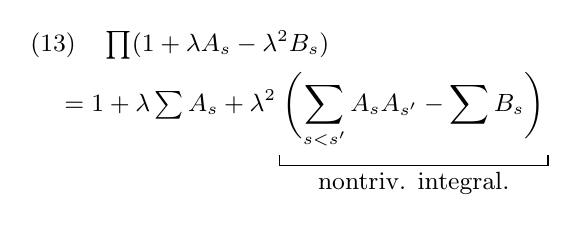
\begin{tikzpicture}[x=1cm,y=1cm,every node/.style={font=\small,inner sep=1pt}]
\node[anchor=base west] at (0,.79)
 {\((13)\quad\prod(1+\lambda A_s-\lambda^2B_s)\)};
\node[anchor=base west] (prefix) at (.43,.03)
 {\(=1+\lambda\sum A_s+\lambda^2\)};
\node[anchor=base west] (coef) at (prefix.base east)
 {\(\displaystyle\biggl(\sum_{s<s'} A_sA_{s'}-\sum B_s\biggr)\)};
\draw ([yshift=-1pt]coef.south west)--([yshift=-5pt]coef.south west)--
 ([yshift=-5pt]coef.south east)--([yshift=-1pt]coef.south east);
\node[below=6pt] at (coef.south) {\uwave{nontriv. integral}.};
\end{tikzpicture}}\endgroup}
\end{GelfandAdjacentEvidence}
\begin{GelfandAdjacentEvidence}{GELFAND-P000792}{4}

\Unclear{GELFAND-P000792}{product-expansions}{Both expansions show equality signs. The subsequent powers are unwritten.}
\end{GelfandAdjacentEvidence}
\begin{GelfandAdjacentEvidence}{GELFAND-P000792}{5}


\[
(14)\qquad \left\{\begin{aligned}
&L_s=e^{-\partial}+A_s+B_s e^\partial\\
&\text{\sout{\ldots}}\qquad M_s=B_s e^\partial
\end{aligned}\right.
\]
\Incomplete{GELFAND-P000792}{equation-14-cancellation}{The entry at the beginning of the second line of (14) is heavily crossed out. Its symbols are illegible.}
\end{GelfandAdjacentEvidence}
\begin{GelfandAdjacentEvidence}{GELFAND-P000792}{6}


Here \(e^\partial\) --- shift by 1 on the lattice

\(L_s,M_s\) --- difference operators (Jacobi matr.)

\underline{Gauge theory.}

\SourceFigure{GELFAND-P000792}{gauge-lattice}{%
\par\begingroup\color{black}\GelfandFitDiagram{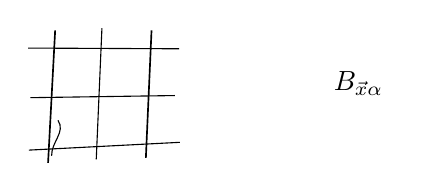
\begin{tikzpicture}[x=.9cm,y=.9cm]
\draw (-.30,0)--(1.83,.11);
\draw (-.28,.74)--(1.76,.77);
\draw (-.31,1.44)--(1.82,1.43);
\draw[semithick] (-.03,-.18)--(.07,1.69);
\draw (.65,-.13)--(.73,1.72);
\draw[semithick] (1.35,-.11)--(1.43,1.69);
\draw (.02,-.08) to[out=91,in=-56] (.11,.42);
\node at (4.35,.94) {\(B_{\vec{x}\alpha}\)};
\end{tikzpicture}}\endgroup}
\end{GelfandAdjacentEvidence}


\(\vec{x}\) --- point, \(\alpha\) --- direction

(\(\alpha=1,\ldots,d\) ---\\
--- \(d\) --- dimension)

2-dim. case --- 2 dir.

(only positive ones are taken)


\Needspace{7\baselineskip}
\begin{GelfandAdjacentEvidence}{GELFAND-P000793}{1}
\SourcePage{GELFAND-P000793}{unlabelled}

\[
(15)\qquad F_{\bar{x}\alpha\beta}=
B_{\bar{x},\alpha} B_{\bar{x}+\bar{\alpha},\beta}
B^{-1}_{\bar{x}+\bar{\beta},\alpha} B^{-1}_{\bar{x},\beta}
\]

Action:
\[
(16)\qquad S=\sum_{\bar{x},\alpha,\beta}\operatorname{Tr} F_{\vec{x}\alpha\beta}
\]
[on the right:] Class. limit \(\longrightarrow F^2\)
\Unclear{GELFAND-P000793}{action-classical-square}{The sign before the raised 2 provisionally reads capital \(F\).}
\end{GelfandAdjacentEvidence}
\begin{GelfandAdjacentEvidence}{GELFAND-P000793}{2}


\SourceFigure{GELFAND-P000793}{action-margin}{%
\par\begingroup\color{black}\GelfandFitDiagram{\begin{tikzpicture}[every node/.style={inner sep=1pt,font=\small}]
\node[anchor=base west] (before) at (0,0) {\(\bigl(e^f=1+\)};
\node[anchor=base west] (linear) at (before.base east) {\(f\)};
\node[anchor=base west] at (linear.base east) {\({}+\tfrac{f^2}{2}\)};
\draw ([yshift=-2pt]linear.south)--([yshift=-9pt]linear.south);
\node[anchor=north west] at ([xshift=-7pt,yshift=-10pt]linear.south) {lin. term canc. \(\bigr)\).};
\end{tikzpicture}}\endgroup}
\end{GelfandAdjacentEvidence}
\begin{GelfandAdjacentEvidence}{GELFAND-P000793}{3}

\Unclear{GELFAND-P000793}{action-exponential}{An equality sign is written in the parenthesis. The series ends after \(f^2/2\).}
\end{GelfandAdjacentEvidence}
\begin{GelfandAdjacentEvidence}{GELFAND-P000793}{4}


\uwave{Eqns. of motion:}

\SourceFigure{GELFAND-P000793}{motion-diagrams}{%
\par\begingroup\color{black}\GelfandFitDiagram{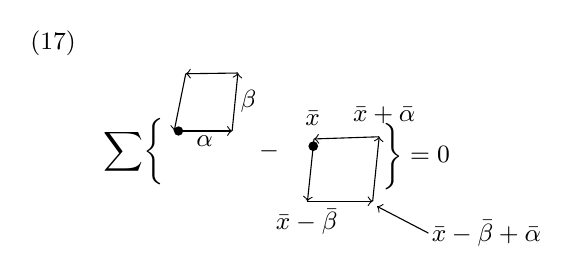
\begin{tikzpicture}[x=.92cm,y=.92cm,every node/.style={font=\small,inner sep=1pt}]
\node[anchor=base west] at (0,1.74) {\((17)\)};
\node at (1.48,.33) {\(\displaystyle\sum\biggl\{\)};
\draw[->] (2.03,.61)--(2.83,.61);
\draw[->] (2.83,.61)--(2.91,1.41);
\draw[->] (2.91,1.41)--(2.19,1.40);
\draw[->] (2.19,1.40)--(2.03,.61);
\fill (2.09,.61) circle (.064);
\node[below] at (2.45,.59) {\(\alpha\)};
\node[right] at (2.9,1.02) {\(\beta\)};
\node at (3.34,.33) {\(-\)};
\draw[->] (4.86,.53)--(3.96,.50);
\draw[->] (3.96,.50)--(3.87,-.36);
\draw[->] (3.87,-.36)--(4.77,-.36);
\draw[->] (4.77,-.36)--(4.86,.53);
\fill (3.95,.40) circle (.067);
\node[above] at (3.94,.64) {\(\bar{x}\)};
\node[above] at (4.93,.67) {\(\bar{x}+\bar{\alpha}\)};
\node[below] at (3.86,-.42) {\(\bar{x}-\bar{\beta}\)};
\node at (5.37,.26) {\(\displaystyle\biggr\}=0\)};
\node[anchor=west] (corner) at (5.54,-.80) {\(\bar{x}-\bar{\beta}+\bar{\alpha}\)};
\draw[->] (corner.west)--(4.83,-.43);
\end{tikzpicture}}\endgroup}
\end{GelfandAdjacentEvidence}
\begin{GelfandAdjacentEvidence}{GELFAND-P000793}{5}


The dot marks the start

\(\sum_\beta\), \(\alpha\) --- fixed\qquad
(\uwave{Cf.:} \(\nabla_\beta F_{\alpha\beta}=0\))
\Unclear{GELFAND-P000793}{motion-comparison-operator}{The overwritten sign provisionally reads \(\nabla\).}
\end{GelfandAdjacentEvidence}
\begin{GelfandAdjacentEvidence}{GELFAND-P000793}{6}


In the 2-dim. case there is no summation.
\Unclear{GELFAND-P000793}{dimension-overwriting}{The abbreviation for “dim.” is retraced. The earlier strokes are indistinct.}
\end{GelfandAdjacentEvidence}
\begin{GelfandAdjacentEvidence}{GELFAND-P000793}{7}


\((17)\) means:
\[
\begin{aligned}
(17)_2\quad \sum\bigl\{&
B_{\bar{x},\alpha}
B_{\bar{x}+\alpha,\beta}
B^{-1}_{\bar{x}+\bar{\beta},\alpha}
B^{-1}_{\bar{x},\beta}\\
&-B^{-1}_{\bar{x}\beta}
B_{\bar{x}-\bar{\beta},\alpha}
B_{\bar{x}-\bar{\beta}+\bar{\alpha},\beta}
B^{-1}_{\bar{x}\alpha}
\bigr\}=0
\end{aligned}
\]
\Unclear{GELFAND-P000793}{expanded-fourth-factor}{The \(\bar{x}\) in the last factor of the first product is retraced.}
\end{GelfandAdjacentEvidence}
\begin{GelfandAdjacentEvidence}{GELFAND-P000793}{8}

\Unclear{GELFAND-P000793}{motion-expanded-first-inverse}{The index in the first inverse factor of the second product reads \(\bar{x}\beta\).}
\end{GelfandAdjacentEvidence}
\begin{GelfandAdjacentEvidence}{GELFAND-P000793}{9}


\SourceFigure{GELFAND-P000793}{closed-contour-18}{%
\par\begingroup\color{black}\GelfandFitDiagram{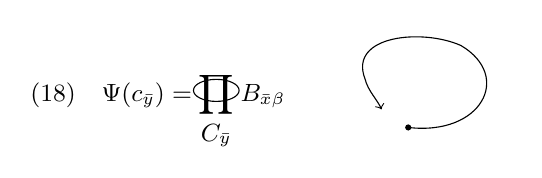
\begin{tikzpicture}[x=1cm,y=1cm,every node/.style={font=\small,inner sep=1pt}]
\node[anchor=base west] (lhs) at (0,0) {\((18)\quad\Psi(c_{\bar{y}})=\)};
\node[anchor=base west] (prod) at (lhs.base east) {\(\displaystyle\prod\)};
\draw ([yshift=4pt]prod.base) ellipse (.29 and .14);
\node[below=0pt] at (prod.south) {\(C_{\bar{y}}\)};
\node[anchor=base west] at (prod.base east) {\(B_{\bar{x}\beta}\)};
\begin{scope}[shift={(4.84,.06)}]
\draw[->] (0,-.39) .. controls (.93,-.50) and (1.33,.26) .. (.67,.65)
 .. controls (.18,.87) and (-.76,.78) .. (-.55,.23)
 .. controls (-.51,.07) and (-.39,-.04) .. (-.34,-.16);
\fill (0,-.39) circle (.039);
\end{scope}
\end{tikzpicture}}\endgroup}
\end{GelfandAdjacentEvidence}
\begin{GelfandAdjacentEvidence}{GELFAND-P000793}{10}

\Unclear{GELFAND-P000793}{contour-18-argument}{The letter in the argument provisionally reads lowercase \(c\). Its \(\bar{y}\) subscript is retraced.}
\end{GelfandAdjacentEvidence}
\begin{GelfandAdjacentEvidence}{GELFAND-P000793}{11}

\Unclear{GELFAND-P000793}{contour-18-product-subscript}{The subscript below the circled product sign provisionally reads \(C_{\bar{y}}\).}
\end{GelfandAdjacentEvidence}
\begin{GelfandAdjacentEvidence}{GELFAND-P000793}{12}

\Unclear{GELFAND-P000793}{contour-18-b-subscript}{The overwritten sign in the subscript of \(B\) provisionally reads \(\bar{x}\).}
\end{GelfandAdjacentEvidence}
\begin{GelfandAdjacentEvidence}{GELFAND-P000793}{13}


Consider
\[
\Psi(c_y+\Pi_{\bar{x}\alpha\beta})
\]
\SourceFigure{GELFAND-P000793}{attached-square}{%
\par\begingroup\color{black}\GelfandFitDiagram{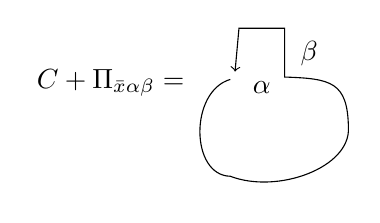
\begin{tikzpicture}[x=1cm,y=1cm]
\node[anchor=east] at (-.86,0) {\(C+\Pi_{\bar{x}\alpha\beta}=\)};
\draw[->] (-.40,.04)
 .. controls (-.92,-.11) and (-.91,-1.18) .. (-.40,-1.19)
 .. controls (.20,-1.42) and (1.13,-1.08) .. (1.10,-.57)
 .. controls (1.09,.01) and (.88,.05) .. (.29,.07)
 -- (.29,.69) -- (-.29,.69) -- (-.34,.14);
\node at (.00,-.06) {\(\alpha\)};
\node[right] at (.37,.37) {\(\beta\)};
\end{tikzpicture}}\endgroup}
\end{GelfandAdjacentEvidence}
\begin{GelfandAdjacentEvidence}{GELFAND-P000793}{14}

a small square has been attached

Now
\[
(19)\qquad\Psi(c+\Pi_{\bar{x}\alpha\beta})\Psi^{-1}(C)=
\]
\SourceFigure{GELFAND-P000793}{transport-19-diagram}{%
\par\begingroup\color{black}\GelfandFitDiagram{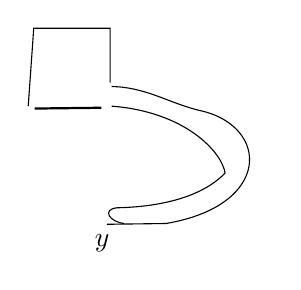
\begin{tikzpicture}[x=1cm,y=1cm]
\draw (-.70,.19)--(-.63,1.18)--(.34,1.18)--(.34,.49);
\draw[thick] (-.62,.16)--(.23,.17);
\draw (.36,.44)
 .. controls (.81,.43) and (1.10,.22) .. (1.50,.13)
 .. controls (2.36,-.07) and (2.40,-1.07) .. (1.05,-1.30)
 -- (.30,-1.31);
\draw (.36,.19)
 .. controls (1.29,.12) and (1.76,-.39) .. (1.80,-.66)
 .. controls (1.49,-.98) and (.94,-1.09) .. (.43,-1.10)
 .. controls (.23,-1.12) and (.33,-1.28) .. (.52,-1.30);
\node[below] at (.24,-1.32) {\(y\)};
\end{tikzpicture}}\endgroup
\par The gaps near the square and the thickened ends are shown. The directions at these points are unclear.}
\end{GelfandAdjacentEvidence}
\begin{GelfandAdjacentEvidence}{GELFAND-P000793}{15}

\Unclear{GELFAND-P000793}{contour-19-case}{The first sign resembles a looped lowercase \(c\). The inverse function has argument \(C\).}
\end{GelfandAdjacentEvidence}
\begin{GelfandAdjacentEvidence}{GELFAND-P000793}{16}

\Unclear{GELFAND-P000793}{contour-19-alpha}{The retraced subscript provisionally reads \(\alpha\).}
\end{GelfandAdjacentEvidence}
\begin{GelfandAdjacentEvidence}{GELFAND-P000793}{17}


dir. at pt. \(\bar{x},\alpha\), transported to point \(y\)

The eqns. are written in the form:
\[
\begin{aligned}
(20)\qquad \sum_\beta\bigl\{&
\Psi(c+\Pi_{\bar{x}\alpha\beta})\Psi^{-1}(C)\\
&-\Psi(C)\Psi^{-1}(C-\Pi_{\bar{x}\alpha\beta})\bigr\}=0
\end{aligned}
\]
\Unclear{GELFAND-P000793}{contour-20-case}{The first contour is provisionally labelled with a lowercase \(c\).}
\end{GelfandAdjacentEvidence}
\begin{GelfandAdjacentEvidence}{GELFAND-P000793}{18}

\Unclear{GELFAND-P000793}{contour-20-overwritten-indices}{The retraced pair of indices provisionally reads \(\alpha\beta\).}
\end{GelfandAdjacentEvidence}
\begin{GelfandAdjacentEvidence}{GELFAND-P000793}{19}


We get something like a connection (trivial) in the space of contours.
(i.e. [inserted above the line:] matrix function of the contour)

(cf. (4))

\uwave{Cont. case.}

\(\Psi[x_{\mu}(s)]\) --- a functional of the curve
(indep. of parametrization)

[on the right:] \(x(s)=(x_\mu(s));\quad \mu=1,2,3,4.\)
\Unclear{GELFAND-P000793}{continuous-overwritten-index}{The retraced subscript of \(x\) provisionally reads \(\mu\).}
\end{GelfandAdjacentEvidence}


Current
\[
(21)\qquad \mathcal{F}_\mu(s,C)=\frac{\delta\Psi(x(s))}{\delta x_\mu(s)}\Psi^{-1}
\]


\Needspace{7\baselineskip}
\begin{GelfandAdjacentEvidence}{GELFAND-P000794}{1}
\SourcePage{GELFAND-P000794}{18}

\uuline{Eqn.:}
\[
(22)_1\qquad\frac{\delta\mathcal{F}_\mu(s,C)}{\delta x_\mu(s)}=0
\]

[on the right]
\SourceFigure{GELFAND-P000794}{group-algebra-bracket}{%
\par\begingroup\color{black}\GelfandFitDiagram{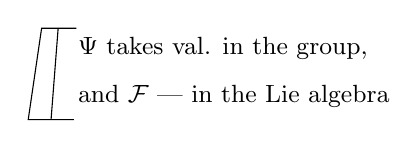
\begin{tikzpicture}[x=1cm,y=1cm,every node/.style={font=\small,inner sep=1pt}]
\node[anchor=west] at (.59,.45) {\(\Psi\) takes val. in the group,};
\node[anchor=west] at (.59,-.16) {and \(\mathcal F\) --- in the Lie algebra};
\draw (.61,.71)--(.17,.71)--(0,-.45)--(.58,-.45);
\draw (.29,-.45)--(.38,.71);
\end{tikzpicture}}\endgroup}
\end{GelfandAdjacentEvidence}
\begin{GelfandAdjacentEvidence}{GELFAND-P000794}{2}


\(\Psi\) is inv. with resp. to parametrization: this is written as
\[
(23)\qquad\frac{dx_\mu}{ds}\frac{\delta\Psi}{\delta x_\mu(s)}=0
\]

\begin{gather*}
\mathcal{F}_\beta=\Psi(c+\Pi_{\alpha\beta})\Psi^{-1}(c)\\
\sum_\beta\{\mathcal{F}_\beta(c)-\mathcal{F}_\beta(c-\Pi_{\alpha\beta})\}=0
\end{gather*}
\Unclear{GELFAND-P000794}{discrete-contour-case}{The letters in the arguments provisionally read lowercase \(c\).}
\end{GelfandAdjacentEvidence}
\begin{GelfandAdjacentEvidence}{GELFAND-P000794}{3}


the cont. limit gives \((22)\).

\[
\Psi=p\,e^{\oint A_\mu\,dx_\mu}
\]
\[
(22)_2\qquad
\frac{\delta\mathcal{F}_\mu(s)}{\delta x_\nu(s')}
-\frac{\delta\mathcal{F}_\nu(s')}{\delta x_\mu(s)}
+[\mathcal{F}_\mu(s),\mathcal{F}_\nu(s')]=0
\]
\Unclear{GELFAND-P000794}{equation-22b-number}{The second digit is overwritten. The upper writing provisionally reads \((22)_2\).}
\end{GelfandAdjacentEvidence}
\begin{GelfandAdjacentEvidence}{GELFAND-P000794}{4}


Action
\[
(24)\qquad S'=\int\left(\frac{\delta\Psi^{-1}}{\delta x_\mu(s)}
\frac{\delta\Psi}{\delta x_\mu(s)}\right)(Dx_\mu(s))
\]
\Unclear{GELFAND-P000794}{action-number}{The second digit combines strokes resembling 4 and 1. Their order is unclear.}
\end{GelfandAdjacentEvidence}
\begin{GelfandAdjacentEvidence}{GELFAND-P000794}{5}

\Unclear{GELFAND-P000794}{action-prime}{The raised stroke to the right of \(S\) is typeset as a prime, \(S'\).}
\end{GelfandAdjacentEvidence}


It is unclear how to define it

\uwave{Carefully:} 3 dimensions.

(in \(4^{\underline{\text{х}}}\) dimensions it has yet to be checked in full).

The eqns. \((22)_1\) --- \((22)_2\) are solved, with \(\mathcal{F}\) obtained from formula (21) and \(\Psi\) satisf. cond. (23).

A Y.–M. field is a chiral field on the space of loops.

On the loops there is a fn. with val. in a finite-dimensional group. For it the eqns. of the principal chir. field (\(\Psi\) is such a field) are (22).

[inserted above the line on the left:] If \(\Psi\) \uwave{comes from a connection}
(\(\Leftrightarrow\) \(\Psi\) --- homom. of loops into the group) \(\Rightarrow\) one gets the Yang–Mills eqns..

\uwave{Currents:} (\(\sim\) integrals of motion):
\[
(25)\qquad
\frac{\delta\mathcal{J}^{(k)}_\mu(s,C)}{\delta x_\mu(s)}=0
\]


\Needspace{7\baselineskip}
\begin{GelfandAdjacentEvidence}{GELFAND-P000795}{1}
\SourcePage{GELFAND-P000795}{unlabelled}

\[
(26)\qquad\mathcal{J}^{(1)}_\mu=\mathcal{F}_\mu(s,C)
\]
\[
(27)\qquad\mathcal{J}^{(2)}_\mu=
\varepsilon_{\mu\nu\lambda}t_\nu(s)\mathcal{F}_\lambda(s,C)
+[\mathcal{F}_\mu(s),\chi]
\]

\(t\) --- tang. vector to the curve

[\sout{\(\mathcal F\)}] \(\chi\) we shall now find
\Unclear{GELFAND-P000795}{cancel-before-chi}{The crossed-out sign resembles \(\mathcal F\).}
\end{GelfandAdjacentEvidence}
\begin{GelfandAdjacentEvidence}{GELFAND-P000795}{2}


We have:
\[
\begin{aligned}
(28)\qquad
\frac{\delta\mathcal{J}^{(2)}_\mu}{\delta x_\mu}
&=\underset{\substack{\Vert\\
\displaystyle\varepsilon_{\mu\nu\lambda}t_\nu[\mathcal{F}_\mu,\mathcal{F}_\lambda]}}
{\varepsilon_{\mu\nu\lambda}t_\nu(s)
\frac{\delta\mathcal{F}_\lambda(s,c)}{\delta x_\mu(s)}}\\[1ex]
&\quad+\left[\mathcal{F}_\mu(s,c),\frac{\delta\chi}{\delta x_\mu(s)}\right]
\end{aligned}
\]
\Unclear{GELFAND-P000795}{derivative-current-glyph}{The letter in the numerator on the left is overwritten. It may read \(\mathcal J\) or \(\mathcal F\).}
\end{GelfandAdjacentEvidence}
\begin{GelfandAdjacentEvidence}{GELFAND-P000795}{3}

\Unclear{GELFAND-P000795}{derivative-identity}{Two vertical strokes connect the first summand with the entry below it. No separate coefficient is visible before \(\varepsilon\) on the lower line.}
\end{GelfandAdjacentEvidence}
\begin{GelfandAdjacentEvidence}{GELFAND-P000795}{4}


Let
\[
(29)\qquad \frac{\delta\chi}{\delta x_\mu}=
-\varepsilon_{\mu\nu\lambda}t_\nu\mathcal{F}_\lambda
\]

Then
\[
(30)\qquad\mathcal{F}_\mu=\varepsilon_{\mu\nu\lambda}t_\nu
\frac{\delta\chi}{\delta x_\lambda}
\]

This is possible if the following holds \((22)_1\)

We obtain a nonlocal conservation law. \quad Expr. \(\chi\):
\Unclear{GELFAND-P000795}{figure-intro}{The abbreviation before \(\chi\) provisionally reads «Выраж-е.» (“expr.”). The dividing stroke is unclear.}
\end{GelfandAdjacentEvidence}
\begin{GelfandAdjacentEvidence}{GELFAND-P000795}{5}


\SourceFigure{GELFAND-P000795}{loop-tail-expansion}{%
\par\begingroup\color{black}\GelfandFitDiagram{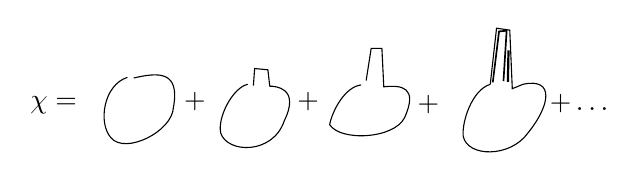
\begin{tikzpicture}[x=.8cm,y=.8cm,every node/.style={inner sep=1pt}]
\node at (0,.30) {\(\chi=\)};
\draw (1.17,.75)
 .. controls (.79,.63) and (.70,.02) .. (.91,-.21)
 .. controls (1.14,-.48) and (1.88,-.11) .. (1.90,.27)
 .. controls (2.01,.86) and (1.66,.83) .. (1.27,.74);
\node at (2.24,.37) {\(+\)};
\draw (3.08,.64)
 .. controls (2.85,.59) and (2.60,.13) .. (2.65,-.13)
 .. controls (2.75,-.46) and (3.48,-.48) .. (3.66,.06)
 .. controls (3.92,.59) and (3.51,.61) .. (3.43,.61)
 -- (3.40,.87)--(3.19,.89)--(3.17,.62);
\node at (4.04,.37) {\(+\)};
\draw (4.88,.63)
 .. controls (4.63,.60) and (4.43,.24) .. (4.38,.00)
 .. controls (4.55,-.27) and (5.40,-.23) .. (5.57,.11)
 .. controls (5.79,.60) and (5.52,.63) .. (5.24,.60)
 -- (5.21,1.21)--(5.04,1.21)--(4.96,.70);
\node at (5.95,.31) {\(+\)};
\draw (6.93,.64)
 .. controls (6.64,.55) and (6.48,.05) .. (6.50,-.18)
 .. controls (6.56,-.52) and (7.25,-.53) .. (7.53,-.13)
 .. controls (7.88,.30) and (7.96,.75) .. (7.45,.64)
 -- (7.28,.57)--(7.24,1.50)--(7.03,1.53)--(6.93,.64);
\draw[semithick] (6.97,.67)--(7.07,1.48)--(7.19,1.49)--(7.14,.69);
\draw[thick] (7.22,1.18)--(7.21,.68);
\node at (8.34,.34) {\(+\ldots\)};
\end{tikzpicture}}\endgroup
\par The short gaps and thickened strokes on the last protrusion are shown. Arrowheads are indistinct.}
\end{GelfandAdjacentEvidence}
\begin{GelfandAdjacentEvidence}{GELFAND-P000795}{6}


(a sq. is added in one direction)

The nonlocality is 1-dimensional.

\uwave{Contours}: 1. S. Mandelstam, Phys. Rev., 1968.

\hspace{1em}2. Minlos, Sinai

[on the right, alongside item 1:] quant. Y.–M. in the spirit of Faddeev–Popov

\uwave{\(\gamma\)-pencil} (instead of the \(L,A\)-pair)
\Unclear{GELFAND-P000795}{pencil-heading-sign}{The overwritten sign in the heading provisionally reads \(\gamma\). \(\lambda\) is also possible.}
\end{GelfandAdjacentEvidence}
\begin{GelfandAdjacentEvidence}{GELFAND-P000795}{7}


\[
(31)\qquad
\frac{\delta\varphi}{\delta x_\mu(s)}
+Z\,\varepsilon_{\mu\nu\lambda}t_\nu\frac{\delta\varphi}{\delta x_\lambda}
=\mathcal{F}_\mu(s,C)\varphi(s,C)
\]
\Unclear{GELFAND-P000795}{equation-31-parameter}{The overwritten parameter resembles a barred \(Z\). Its letter case is unclear.}
\end{GelfandAdjacentEvidence}
\begin{GelfandAdjacentEvidence}{GELFAND-P000795}{8}


\(Z\) --- arbitrary parameter
\Unclear{GELFAND-P000795}{parameter-note}{The letter in the explanation has a similar shape. Its case is unclear.}
\end{GelfandAdjacentEvidence}
\begin{GelfandAdjacentEvidence}{GELFAND-P000795}{9}


The following has an analog. form:

\uwave{Std. chiral field}: (Pohlmayer, Zakharov, Mikhailov):
\[
\begin{aligned}
(32)\qquad A_\mu&=g^{-1}\partial_\mu g(x);\\
\left[\partial_\mu+Z\,\varepsilon_{\mu\nu}\partial_\nu\right]\varphi
&=A_\mu\varphi,\qquad\mu=1,2,\,..
\end{aligned}
\]
\Unclear{GELFAND-P000795}{equation-32-parameter}{The letter before \(\varepsilon\) provisionally reads \(Z\). Its case is unclear.}
\end{GelfandAdjacentEvidence}



\Needspace{7\baselineskip}
\begin{GelfandAdjacentEvidence}{GELFAND-P000796}{1}
\SourcePage{GELFAND-P000796}{19}

\((31)\) --- a system of eqns., \(Z\) --- spectral param.
\Unclear{GELFAND-P000796}{spectral-parameter-first}{The letter in the explanation is retraced and resembles a barred \(Z\). Its case is unclear.}
\end{GelfandAdjacentEvidence}
\begin{GelfandAdjacentEvidence}{GELFAND-P000796}{2}


Compatibility of \((31)\Rightarrow\) eqns. \((22)\).
\[
Z=0\quad\Rightarrow\quad\varphi=\Psi
\]
\Unclear{GELFAND-P000796}{spectral-parameter-zero}{The letter before \(=0\) is retraced and resembles a barred \(Z\). In the following formulas the letter is written smaller.}
\end{GelfandAdjacentEvidence}
\begin{GelfandAdjacentEvidence}{GELFAND-P000796}{3}


\uwave{Integrals} --- ?

In model (32) let us see how the integrals are obtained.
\[
(32)\Leftrightarrow
\]
\[
(33)\qquad\partial_\mu\varphi
=\frac{A_\mu+z\varepsilon_{\mu\nu}A_\nu}{1-z^2}\,\varphi
\]
\[
(34)\qquad P\exp\oint_C\frac{A_\mu+z\varepsilon_{\mu\nu}A_\nu}{1-z^2}\,dx^\mu=1
\]
(ord. expon)

Spec. choice of contour:
\SourceFigure{GELFAND-P000796}{contour-01}{%
\par\begingroup\color{black}\GelfandFitDiagram{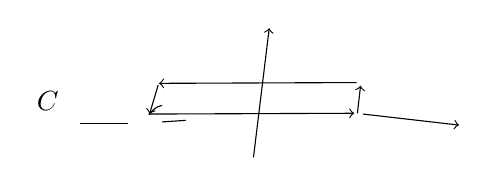
\begin{tikzpicture}[x=1cm,y=1cm]
\node[left] at (-2.54,.13) {\(C\)};
\draw (-2.39,-.15)--(-1.78,-.15);
\draw[->] (1.20,-.03)--(2.42,-.17);
\draw[->] (-.19,-.58)--(.01,1.06);
\draw[->] (1.12,.37)--(-1.39,.36);
\draw[->] (-1.40,.34)--(-1.51,-.03);
\draw[->] (-1.51,-.03)--(1.09,-.02);
\draw[->] (1.13,-.02)--(1.17,.33);
\draw (-1.35,-.13)--(-1.05,-.11);
\draw (-1.52,-.04) to[out=50,in=-170] (-1.35,.08);
\end{tikzpicture}}\endgroup
\par Additional strokes appear at the lower left corner. Their purpose is unclear.}
\end{GelfandAdjacentEvidence}
\begin{GelfandAdjacentEvidence}{GELFAND-P000796}{4}


\[
(35)\qquad\frac{d}{dt}\,P\exp\int_{-\infty}^{\infty}dx_1
\left\{\frac{A_1+zA_2}{1-z^2}\right\}=0
\]
This is the generating \underline{fn. of the integrals} of motion.

The usual relations carry over to “contourology.”

There are Feynman diagrs. with surfaces in place of lines.

For free field theory
\SourceFigure{GELFAND-P000796}{propagator-line}{%
\par\begingroup\color{black}\GelfandFitDiagram{\begin{tikzpicture}[x=1cm,y=1cm]
\fill (0,0) circle (.027);
\draw[->] (.12,0)--(2.35,0);
\node[below] at (.13,-.09) {\(x\)};
\node[below right] at (2.58,-.08) {\(x'\)};
\end{tikzpicture}}\endgroup}
\end{GelfandAdjacentEvidence}
\begin{GelfandAdjacentEvidence}{GELFAND-P000796}{5}

the Green fn. \(G(x,x')\) satisfies the K.–G. eqn.
\[
(36)\qquad (\partial_x^2-m^2)G(x,x')=\delta(x-x')
\]
\[
(37)\qquad G(x,x')\underset{|x-x'|\to\infty}{\sim}e^{-m|x-x'|}
\]

Here on contours
\[
(38)\qquad \left\{\frac{\delta^2}{\delta x_\mu^2(s)}
-m^4\left(\frac{dx_\mu}{ds}\right)^2\right\}G(C)=0
\]
\Unclear{GELFAND-P000796}{string-denominator}{The overwritten denominator provisionally reads \(ds\).}
\end{GelfandAdjacentEvidence}

\[
(39)\qquad G(C)=\langle\Psi(C)\rangle
\]

How does one find the contour Green fn.?

\uwave{Math. problem:} \((38)\) --- the “string” K.–G. eqn.

Boundary cond.: decay for large contours:
\[
(40)\qquad G(C)\sim e^{-m^2 A(C)}
\]
(\(A(C)\) --- min. area spanning the contour \(C\))


\Needspace{7\baselineskip}
\begin{GelfandAdjacentEvidence}{GELFAND-P000797}{1}
\SourcePage{GELFAND-P000797}{unlabelled}

Let \(G\) depend only on the tensors
\[
(41)\qquad \sigma_{\alpha\beta}=\oint_C x_\alpha\,dx_\beta
\]
\[
(42)\qquad \frac{\delta\sigma_{\alpha\beta}}{\delta x_\mu(s)}
=\delta_{\alpha\mu}\frac{dx_\beta}{ds}-\delta_{\beta\mu}\frac{dx_\alpha}{ds}
\]
\[
t_\mu(s)=\frac{dx_\mu}{ds}
\]
\[
(43)\qquad \text{\sout{\ldots}}\ t_\alpha t_\beta
\left[\frac{\partial^2}{\partial\sigma_{\alpha\gamma}\partial\sigma_{\beta\gamma}}
-m^4\delta_{\alpha\beta}\right]G=0
\]
\Unclear{GELFAND-P000797}{eq43-cancel}{The crossed-out entry before \(t_\alpha t_\beta\) resembles a summation sign with subscripts.}
\end{GelfandAdjacentEvidence}
\begin{GelfandAdjacentEvidence}{GELFAND-P000797}{2}


Let
\[
\pi_{\alpha\beta}=\frac{\partial}{\partial\sigma_{\alpha\beta}}
\]

Then we obtain
\[
(44)\qquad \pi_{\alpha\beta}\pi_{\beta\gamma}
=\text{\sout{\(\tfrac14\pi^2_{\ldots}\delta_{\ldots}\)}}\quad C\delta_{\alpha\beta};
\]
\Unclear{GELFAND-P000797}{eq44-cancel}{The crossed-out signs after the equals sign resemble \(\frac14\), \(\pi^2\) and \(\delta\). Their subscripts are unclear.}
\end{GelfandAdjacentEvidence}
\begin{GelfandAdjacentEvidence}{GELFAND-P000797}{3}

\Unclear{GELFAND-P000797}{eq44-indices}{The subscripts of the uncrossed \(\delta\) on the right read \(\alpha\beta\).}
\end{GelfandAdjacentEvidence}
\begin{GelfandAdjacentEvidence}{GELFAND-P000797}{4}


This is possible only when
\[
(45)\qquad \pi_{\alpha\beta}=\pm{}^*\pi_{\alpha\beta}
=\pm\varepsilon_{\alpha\beta\gamma\delta}\pi_{\gamma\delta}
\]

Hence a fn. only of
\[
(46)\qquad U_\pm=\sqrt{\sigma_{\alpha\beta}^2
\pm\sigma_{\alpha\beta}\,{}^*\sigma_{\alpha\beta}}
\]

Explicit solution:
\[
G(U_+,U_-)
\]
expressed via Bessel fns.

[between the lines:] Look at infinity:

Min. area
\[
(47)\qquad A_{\min}(C)=\sqrt{\sigma^2\pm\sigma\,{}^*\sigma}
\]
\(\sigma\) --- projection onto coord. planes
\[
\sigma_{\alpha\beta}=\oint x_\alpha\,dx_\beta
\]
\[
A=\int\sqrt{\dot{x}^{\,2}x'^{\,2}-(\dot{x}x')^2}\,dt\,ds
\]

The Euler eqn. gives
\[
A_{\min}(x(s))
\]
\Unclear{GELFAND-P000797}{final-argument}{The signs of the argument on the last line are retraced. They provisionally read \(x(s)\).}
\end{GelfandAdjacentEvidence}



\Needspace{7\baselineskip}
\begin{GelfandAdjacentEvidence}{GELFAND-P000798}{1}
\SourcePage{GELFAND-P000798}{20}

Ham.–Jacobi eqn.
\[
\left(\frac{\delta A_{\min}}{\delta x_\mu(s)}\right)^2
=\left(\frac{dx_\mu}{ds}\right)^2
\]

We find a solution. (47) --- satisfies the Ham.–Jacobi eqn.

For contours that are not too [\sout{\ldots}] twisted, \((47)\) --- a solution.
\Incomplete{GELFAND-P000798}{text-cancel}{A short entry between “too” and “twisted” is crossed out. The letters are indistinct.}
\end{GelfandAdjacentEvidence}


Sinai asserts that Courant has something.


\Needspace{7\baselineskip}
\begin{GelfandAdjacentEvidence}{GELFAND-P000799}{1}
\SourcePage{GELFAND-P000799}{unlabelled}

\underline{\underline{20.11.78.}}\qquad\underline{\underline{Gelfand Sem.}}

\SourceFigure{GELFAND-P000799}{palindrome-bracket}{%
\par\noindent
\(\left.\vcenter{\hbox{\scriptsize\shortstack[l]{%
«Торт с кофе не фокстрот»\\
«Сенсация: поп яйца снес»\\
«Я иду с мечем судия»}}}\right]\)
\enspace{\scriptsize\uwave{Palindromes.}}
\par\smallskip Cake with coffee is no foxtrot. Sensation: a priest laid eggs. I go with a sword, O judge.}
\end{GelfandAdjacentEvidence}
\begin{GelfandAdjacentEvidence}{GELFAND-P000799}{2}


\uwave{Krichever:} instantons without bundles.

\underline{\underline{A. S. Schwarz.}}

1. \uwave{Quantum} [inserted above the line: \uwave{field theory and}]
\uwave{stat. phys.} --- the science of computing the integral (partition function)
\begin{equation*}
Z=\int e^{-S(A)}\,dA
\tag{1}
\end{equation*}
\(A\) ranges over the space of trajectories or histories: \uwave{\(A=A(x,t)\)}.

\uwave{Meaning:} we replace it by a finite-dimensional one (lattice approx.) and pass to the limit; \(a\) --- [\sout{\ldots}] lattice spacing.
\Unclear{GELFAND-P000799}{step-cancel}{A short word before “lattice spacing” is crossed out. It may read «шаг» (“step”).}
\end{GelfandAdjacentEvidence}
\begin{GelfandAdjacentEvidence}{GELFAND-P000799}{3}


\uwave{QFT:} the limit as \(a\to0\) does not exist.
\SourceFigure{GELFAND-P000799}{uv-arrow}{%
\par (ultraviolet divergences)
\par\hspace{1em}\tikz[baseline=-.2ex]{\draw[<->] (0,0)--(.23,.31);}
\par lattice --- momentum cutoff.}
\end{GelfandAdjacentEvidence}
\begin{GelfandAdjacentEvidence}{GELFAND-P000799}{4}


One way out is to take the limit for correl. fns., i.e. to compute
\begin{equation*}
\frac{\int\varphi(A)e^{-S(A)}\,dA}{\int e^{-S(A)}\,dA}
\tag{2}
\end{equation*}
(Green fns. or correlation fns.).

\uwave{Important:} the limit of the ratio already makes sense.

\underline{Also:} when removing the cutoff one must do “renormalization”, i.e. the parameter \(\lambda_a\) must be varied as a function of \(a\) when passing to the limit.

\uwave{There are 2 methods for computing cont. integrals:}

\underline{perturbation theory} and \underline{semiclassics}

(in fact the 1st is a special case).

\uwave{An important class of functionals} \(S\), \uwave{which turns out to be}
\underline{\underline{degenerate}},
i.e. admitting an \(\infty\)-dimensional symmetry group:
\Unclear{GELFAND-P000799}{degeneracy-word}{The abbreviation before «вырожденным» (“degenerate”) reads «оказ.». A faint dot is visible before the comma after the word.}
\end{GelfandAdjacentEvidence}
\begin{GelfandAdjacentEvidence}{GELFAND-P000799}{5}

\[
g\in G\quad\leadsto\quad A\mapsto A^g
\]
\begin{equation*}
\underline{S(A^g)=S(A)}
\tag{3}
\end{equation*}

\uwave{Physical examples:} gauge theories.

Pure Y.–M. theory; \(A=(A_\mu(x))\), \(A_\mu\in\) Lie alg. of a finite-dimensional Lie group.
\begin{equation*}
S(A)=\int\langle F_{\mu\nu},F^{\mu\nu}\rangle\,dV,
\tag{4}
\end{equation*}
where
\begin{equation*}
F_{\mu\nu}=\partial_\mu A_\nu-\partial_\nu A_\mu+[A_\mu,A_\nu]
\tag{5}
\end{equation*}
\Unclear{GELFAND-P000799}{curvature-index}{The subscript of the second \(\partial\) is heavily retraced. It provisionally reads \(\nu\).}
\end{GelfandAdjacentEvidence}



\Needspace{7\baselineskip}
\begin{GelfandAdjacentEvidence}{GELFAND-P000800}{1}
\SourcePage{GELFAND-P000800}{26}

\uwave{Symmetry group:}

if \(g(x)\) --- a fn. with values in the Lie group,
then it generates a transformation of the fields
\begin{equation*}
A_\mu\mapsto g A_\mu g^{-1}+g\,\partial_\mu(g^{-1})
\tag{6}
\end{equation*}
[crossed out above the next line: \sout{\ldots}]
\Incomplete{GELFAND-P000800}{upper-cancel}{A short entry above «Способ» (“Method”) is obscured by heavy hatching.}
\end{GelfandAdjacentEvidence}
\begin{GelfandAdjacentEvidence}{GELFAND-P000800}{2}


\uwave{Method for dealing with degeneracy. In the case of the electromagn. field.}

“The potentials have no meaning”, let us impose a gauge condition
\begin{equation*}
\partial_\mu A_\mu=0
\tag{7}
\end{equation*}
\uwave{Difficulties:} it is hard to construct a perturbation theory.

2. \uwave{Semiclassics} \(\sim\) stationary phase or Laplace method.

a) A problem solved long ago: how to write the cont. integral (\uwave{Faddeev and Popov})

[below the line:] --- at the physicist’s level of rigor.

b) Math. theory --- when \(S\) is quadratic.

c) Application to computing the instanton contribution.

d) Ray–Singer invariants.

a) \underline{Quantization of degen. Lagrangians}.

\uline{Difficulty:} the integral diverges, since the volume of the orbits is infinite.

\uwave{moral:} choose a gauge condition --- a transversal to the orbits --- and integrate over it.

\SourceFigure{GELFAND-P000800}{orbits-01}{%
\par\begingroup\color{black}\GelfandFitDiagram{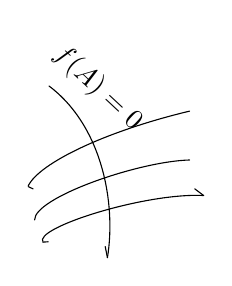
\begin{tikzpicture}[x=.94cm,y=.94cm,line cap=round,line join=round]
\draw (0,.61).. controls (.15,.92) and (1.05,1.35)..(2.18,1.62);
\draw (0,.60)--(.065,.57);
\draw (.086,.15).. controls (.08,.45) and (1.48,.94)..(2.18,.96);
\draw (.20,-.15).. controls (.06,.04) and (1.58,.52)..(2.37,.48);
\draw (.20,-.15)--(.27,-.145);
\draw (2.25,.57)--(2.37,.48);
\draw (.28,1.96).. controls (1.00,1.42) and (1.19,.37)..(1.07,-.36);
\draw (1.04,-.21)--(1.07,-.36);
\node[rotate=-43] at (.94,1.93) {\(f(A)=0\)};
\end{tikzpicture}}\endgroup
\par Angled strokes are visible at the right end of the lowest curve and the bottom of the transverse curve. The redraw shows the visible sides of those strokes.}
\end{GelfandAdjacentEvidence}
\begin{GelfandAdjacentEvidence}{GELFAND-P000800}{3}


but: one must insert the factor \(\underline{\underline{\delta(f(A))}}\).

In addition, one must insert the Jacobian \(\Delta_f(A)\)
\begin{equation*}
\underline{\underline{\Delta_f(A)\delta(f(A))}}
\tag{8}
\end{equation*}
The F.–P. method is to compute \(\Delta_f(A)\). (he does not go into this)

\(\underline{\underline{f(A)=0}}\) --- eqn. of the transversal.

For finite-fold integrals, here --- \underline{\underline{a theorem}}.

[added on the left:] \underline{Another method.}

Let us consider the integral again (in the finite-fold case)
\begin{equation*}
\int_M e^{-S(A)}\,dA
=\int_{M/G}e^{-S(A)}\det(TT^*)^{1/2}\,dV,
\tag{9}
\end{equation*}
\Unclear{GELFAND-P000800}{eq9-determinant}{Equation (9) reads \(\det(TT^*)^{1/2}\). No prime is visible on \(\det\).}
\end{GelfandAdjacentEvidence}


where \(dV\) --- the measure on the set of orbits, obtained from the \uwave{std. Riem. metric} on it.

\(T\) --- the operator obtained as follows: take (assuming the action free):
\[
T:\underset{\substack{\vert\\\text{Lie alg.}}}{\mathfrak g}
\xrightarrow{T_x}T_x(M)
\]
[on the right:] map obtained from the group action.

Assume that \(G\) acts by isometries on \(M\).


\Needspace{7\baselineskip}
\begin{GelfandAdjacentEvidence}{GELFAND-P000801}{1}
\SourcePage{GELFAND-P000801}{unlabelled}

In physics the problem arises of computing by Laplace’s method, i.e. of finding the asymptotics of
\begin{equation*}
\int e^{-\frac{1}{\alpha}S'(A)}\,dA\qquad
\text{as }\alpha\to0
\tag{10}
\end{equation*}
\Unclear{GELFAND-P000801}{exp-action}{A separate short stroke follows \(S\) in the exponent of (10). It is provisionally read as \(S'\).}
\end{GelfandAdjacentEvidence}
\begin{GelfandAdjacentEvidence}{GELFAND-P000801}{2}


One needs to know the stat. points of \(S'(A)\), called \uwave{instantons}.
\Unclear{GELFAND-P000801}{stationary-action}{The short stroke before the opening parenthesis is provisionally read as a prime on \(S\).}
\end{GelfandAdjacentEvidence}
\begin{GelfandAdjacentEvidence}{GELFAND-P000801}{3}


The math. problem is as follows. There is a set of stat. points (even several manifolds), and even \(\infty\)-dimensional ones. There is also strong degeneracy.

\underline{Examples:}

1) Y.–M. field.\qquad \(G=SU(2)\)

\(\forall q\) there is a family of \(8q-3\) instantons apart from the \(\infty\)-dimensional symmetry.

\begin{equation*}
2)\qquad S(\vec n)=\frac{1}{f_0}\int(\partial_\mu\vec n)^2
\ \text{\sout{\ldots}}\ d^2x,
\quad \mu=0,1;\quad x=(x_0,x_1)
\tag{11}
\end{equation*}
\Incomplete{GELFAND-P000801}{eq11-cancel}{An entry between \((\partial_\mu\vec n)^2\) and \(d^2x\) is heavily crossed out. A loop is visible at the left. The entry itself is illegible.}
\end{GelfandAdjacentEvidence}
\begin{GelfandAdjacentEvidence}{GELFAND-P000801}{4}


One has to compute Gaussian integrals, and there arises \(\underline{\underline{\det}}\).

A degen. Lagrangian gives one more \(\det\) --- from Faddeev–Popov --- it is \(\underline{\det(TT^*)^{1/2}}\).

The determinants are \(\infty\)-dimensional. They require analytic continuation or renormalization.

And they turn out to depend on the choice of metric.

But one can trace the change in \(\det\) under variation of the metric.

In \((11)\): \(\vec n=(n_1,n_2,n_3)\in S^2,\quad |\vec n|=1\).

The extremals in \((11)\) were found by \uwave{Belavin and Polyakov}.

Let us pass to stereogr. variables on the plane --- to the sphere.

We obtain \(\underline{\underline{w(z)}}\).

\underline{Answer:} \uwave{extremals}
\(\leftrightarrow\) \(w(z)\) --- \uwave{rational fns. of} \(z\)!

\uwave{Explanation:} there is a top. number \(N\) --- the degree of the map

(\(\sim\) integral of the Jacobian).

Then a simple calculation shows
\begin{equation*}
S'=c_1N+c_2\int\frac{1}{(1+|w|^2)^2}
\left|\frac{\partial w}{\partial\bar z}\right|^2,
\tag{12}
\end{equation*}
\Unclear{GELFAND-P000801}{eq12-measure}{A short stroke is visible beside \(S\) on the left of (12). It is provisionally read as \(S'\). No differential is visible after the squared modulus.}
\end{GelfandAdjacentEvidence}


from which everything follows.

One must compute \(\det\).

There is no gauge group here and there is one \(\det\). The asympt. of (10) is given by the integral
\begin{equation*}
\int\det^{-1/2}(\ldots)\,d\mu_0,
\tag{13}
\end{equation*}
where \(\mu_0\) --- some measure on instantons.

\sout{It turns out to be convenient}

The operator is constructed from \(\forall\) rational fn. as the
[inserted above the line: op. of the quadr. form corresp. to] the principal quadr. part of the f’nal
\[
z=x_0+ix_1
\]
\begin{equation*}
z\xrightarrow{w}\mathrm{CP}(1)
\tag{14}
\end{equation*}


\Needspace{7\baselineskip}
\begin{GelfandAdjacentEvidence}{GELFAND-P000802}{1}
\SourcePage{GELFAND-P000802}{27}

\(T\mathrm{CP}(1)\) induces a bundle on the \(z\)-plane (by this map).

[below \(T\mathrm{CP}(1)\):] (holomorphic)

[on the right:] \(w\) --- rat'l.
\begin{equation*}
\Delta=\bar\partial^{\,*}\bar\partial,\qquad
\bar\partial=\frac{\partial}{\partial\bar z}:\Lambda^{0,0}\to\Lambda^{0,1}
\tag{15}
\end{equation*}
[under the right-hand part:] \uwave{on forms with values in the bundle}.

The metric also depends on \(w\).

(induced by the std. metric of \(\mathrm{CP}^{1}\))

\(w\) actually enters only in the \(*\).

\uwave{One has to compute} \(\det\). This is done using the general theory.

[crossed-out block: \sout{\ldots}]
\Incomplete{GELFAND-P000802}{upper-cancel-block}{Dense horizontal and diagonal strokes fill the outlined block. The underlying entry is illegible.}
\end{GelfandAdjacentEvidence}
\begin{GelfandAdjacentEvidence}{GELFAND-P000802}{2}


\(\det\) is regularized, simultaneously renormalizing \(f_0\) (coupling const.) in \((11)\).

One way to regularize is to consider

[crossed out: \sout{\(\zeta(A)=\)}]
\Unclear{GELFAND-P000802}{eq16-cancel}{The crossed-out entry is provisionally read as \(\zeta(A)=\). Cancellation strokes intersect its ending.}
\end{GelfandAdjacentEvidence}
\begin{GelfandAdjacentEvidence}{GELFAND-P000802}{3}

\begin{equation*}
\zeta(s)=\sum_{\lambda_i\ne0}\lambda_i^{-s}
\tag{16}
\end{equation*}
\(s=0\) --- point of analyticity.
\begin{equation*}
\underline{\ln\det\underset{\mathrm{def}}{=}-\zeta'(0)}.
\tag{17}
\end{equation*}

The op. \(\bar\partial\) is “one and the same” for all instantons with the same top. number \(N\).

\uwave{General statement:} --- when the metric changes, one can trace the change in
\[
\det(A^*A)
\]
idea:

[\sout{\(\frac{d}{du}\operatorname{Sp}e^{-tA^*A}\)}]
\Unclear{GELFAND-P000802}{heat-variation-cancel}{The crossed-out entry is provisionally read as \(\frac{d}{du}\operatorname{Sp}e^{-tA^*A}\). Diagonal strokes intersect the exponent and denominator.}
\end{GelfandAdjacentEvidence}
\begin{GelfandAdjacentEvidence}{GELFAND-P000802}{4}

\begin{equation*}
\frac{d}{du}A^*A=BA^*A+A^*CA
\tag{18}
\end{equation*}
Here \(B\) arises from the formula giving the variation of the scalar product:
\begin{equation*}
(u,v)=\langle u,v\rangle+\langle Bu,v\rangle.
\tag{19}
\end{equation*}

The variation of \(\det A^*A\) will be expressed in terms of
\(\underline{\operatorname{Sp}e^{-tA^*A}}\) using the Frullani integral.

[crossed out above the next formula: \sout{\(\ln\det A=\)}]
\Unclear{GELFAND-P000802}{eq20-cancel}{The crossed-out line is provisionally read as \(\ln\det A=\). The final strokes are obscured.}
\end{GelfandAdjacentEvidence}
\begin{GelfandAdjacentEvidence}{GELFAND-P000802}{5}

\begin{equation*}
\int_0^\infty\frac{e^{-ta}-e^{-tb}}{t}\,dt=\ln\frac ba
\tag{20}
\end{equation*}
(Frullani integral).

or:
\begin{equation*}
\ln\det A=
\left(\int_\varepsilon^\infty\operatorname{Sp}e^{-tA^*A}\frac{dt}{t}\right)_{\text{reg. part as }\varepsilon\to+0}
\tag{21}
\end{equation*}
\Unclear{GELFAND-P000802}{eq21-sign}{The left side of (21) reads \(\ln\det A\). No minus sign or numerical factor is visible before the integral.}
\end{GelfandAdjacentEvidence}



\Needspace{7\baselineskip}
\begin{GelfandAdjacentEvidence}{GELFAND-P000803}{1}
\SourcePage{GELFAND-P000803}{unlabelled}

\begin{equation*}
\begin{aligned}
\frac{d}{du}\operatorname{Sp}e^{-tA^*A}
&=-t\operatorname{Sp}\bigl[(BA^*A+A^*CA)e^{-tA^*A}\bigr]=\\
&=t\frac{d}{dt}\operatorname{Sp}\bigl[Be^{-tA^*A}\bigr]
 +\operatorname{Sp}\bigl[Ce^{-tAA^*}\bigr]
\end{aligned}
\tag{22}
\end{equation*}
\Unclear{GELFAND-P000803}{eq22-scope}{In the second line of (22) the bracket after the trace with \(B\) closes before the plus sign. The trace with \(C\) is written separately, with no visible \(t\,d/dt\).}
\end{GelfandAdjacentEvidence}
\begin{GelfandAdjacentEvidence}{GELFAND-P000803}{2}


\(t\) --- cancels with \(\frac{1}{t}\) in \((21)\)

and integrals come out, the corresp. coeffs. of the Seeley asympt.
\[
\ln\det A=\int_\varepsilon^\infty\operatorname{Sp}e^{-tA^*A}\frac{dt}{t}
 +\sum a_i\varepsilon^i+a_0\ln\varepsilon.
\]
\underline{\underline{What matters is \(a_0\)}}.

\(t\to\infty\quad\Rightarrow\quad\) \uwave{zero modes}.

this part is left unevaluated.

One has to compute the integral with respect to \(d\mu_0\).

\(d\mu_0\) has to be computed too! --- \uwave{it is an \(n\)-dimensional \(\det\)}

One has to compute the \((4q+2)\)-dimensional \(\det\) of the metric tensor.

The metric on rat’l fns. comes from the std. metric on all fns. (in their tangent space) \(=\sum\) squares of variations.

In fact the \textbf{2} unevaluated parts (from the modes and from \(d\mu_0\)) cancel!!

One still has to compute
\[
\int\Phi(\vec n)\det^{-1/2}(\ldots)\,d\mu_0.
\]
Specify a rat’l fn. by its zeros and poles.
\[
\begin{array}{ll|l}
a_1\ldots a_n&\text{--- zeros}&c\text{ --- asympt. at }\infty.\\
b_1\ldots b_n&\text{--- poles}&
\end{array}
\]
\[
\frac{
 \displaystyle\sum_q\int\varphi(\vec n)
 \frac{\prod |a_i-a_j|^2|b_i-b_j|^2}
 {\prod_{1\le i\le q}|a_i-b_j|^2}
 \frac{1}{(1+|c^2|)^2}\ldots
}{\displaystyle\sum_q\ldots}
\]
\Unclear{GELFAND-P000803}{ratio-indices}{The upper product has no written limits. The lower one has \(1\le i\le q\) beneath it, while both \(i\) and \(j\) occur in the factor. The exponent in \(|c^2|\) is inside the modulus bars.}
\end{GelfandAdjacentEvidence}
\begin{GelfandAdjacentEvidence}{GELFAND-P000803}{3}

\[
\varphi(\vec n)=n_\alpha(z')n_\beta(z'')
\]
The denominator is the partition function of a Coulomb gas in the plane.

At poles --- \(+\) charges

\hspace{1em}at zeros --- \(-\) charges.

[on the right:]
\[
\left(\prod_{\ldots}=\text{\sout{\ldots}}\ e^{\sum\ln\ldots}\right)
\]
\Incomplete{GELFAND-P000803}{lower-cancel}{The sign before \(e\) is heavily crossed out. Angled strokes remain visible and the sign is illegible.}
\end{GelfandAdjacentEvidence}
\begin{GelfandAdjacentEvidence}{GELFAND-P000803}{4}


At one value of the temp. (that very one!) this is equiv. to free \uwave{fermions}.

[inserted below: the one we have]
\Unclear{GELFAND-P000803}{temperature-antecedent}{The abbreviation in the note below the parenthesis is provisionally read as «к-рое» (“which”, referring to the value).}
\end{GelfandAdjacentEvidence}



\Needspace{7\baselineskip}
\begin{GelfandAdjacentEvidence}{GELFAND-P000804}{1}
\SourcePage{GELFAND-P000804}{unlabelled}

\underline{\underline{27.11.78.}}\qquad\underline{Gelfand Sem.}

\uwave{Lev Nikolaevich Lipatov}

on the asympt. of diagrams.

\underline{\underline{Zakharov}}.

\uwave{For integrable systems “in general position” the var. principle will hold}.

(all the known ones are out of general position)
\begin{equation*}
\begin{cases}
\Psi_\xi=U\Psi\\
\Psi_\eta=V\Psi
\end{cases}
\tag{1}
\end{equation*}
\[
\left.\begin{aligned}
U&=U(\xi,\eta,\lambda)\\
V&=V(\xi,\eta,\lambda)
\end{aligned}\right\}\quad\text{rat’l fns. in }\lambda
\]
\begin{equation*}
\begin{cases}
\displaystyle U=U_0+\sum_{n=1}^{N_1}\frac{U_n}{\lambda-\lambda_n},\\[1ex]
\displaystyle V=V_0+\sum_{n=1}^{N_2}\frac{V_n}{\lambda-\mu_n}
\end{cases}
\tag{2}
\end{equation*}
\[
\lambda_i\ne\lambda_j;\qquad\mu_i\ne\mu_j;\qquad\lambda_n\ne\mu_m
\]
\(\Psi,U,V\) --- matrices

Int. system:
\begin{equation*}
U_\xi-V_\eta+[U,V]=0
\tag{3}
\end{equation*}
\Unclear{GELFAND-P000804}{eq3-indices}{In (3) the subscript on \(U\) is \(\xi\), and the one on \(V\) is \(\eta\).}
\end{GelfandAdjacentEvidence}


\uwave{Lax pairs:} \(U\) has a simple pole at the \(1^{\text{st}}\) point,
\(V\) has a pole of any order at that same point


\Needspace{7\baselineskip}
\begin{GelfandAdjacentEvidence}{GELFAND-P000805}{1}
\SourcePage{GELFAND-P000805}{37}

[crossed out at the start of the line: \sout{\ldots}]
\Incomplete{GELFAND-P000805}{top-cancel}{Several horizontal strokes cover a short word. Its letters are indistinct.}
\end{GelfandAdjacentEvidence}
\begin{GelfandAdjacentEvidence}{GELFAND-P000805}{2}


Then \(U,V\) can be made into polynomials:
\[
U=U_0+U\lambda
\]
\[
V=P_n(\lambda)
\]
\Unclear{GELFAND-P000805}{top-u-coefficient}{No subscript is visible on the \(U\) before \(\lambda\).}
\end{GelfandAdjacentEvidence}
\begin{GelfandAdjacentEvidence}{GELFAND-P000805}{3}


In more detail, \((3)\) has the form:
\begin{equation*}
\begin{cases}
U_{0\eta}-V_{0\xi}+[U_0,V_0]=0\\
U_{n\eta}=[U_n,A_n]\\
V_{n\xi}=[V_n,B_n]
\end{cases}
\tag{4}
\end{equation*}
Here
\begin{equation*}
A_n=V\big|_{\lambda=\lambda_n},\qquad
B_n=U\big|_{\lambda=\mu_n}.
\tag{5}
\end{equation*}

This is a syst. of \(N_1+N_2+1\) eqns. for \(N_1+N_2+2\) quantities.

Let us integrate partially. Let \(U_n^{(0)}\) and \(V_n^{(0)}\) --- Jordan forms,
then
\begin{equation*}
U_n^{(0)}=U_n^{(0)}(\xi),\qquad
V_n^{(0)}=V_n^{(0)}(\eta)
\qquad\text{(by \((4)_{2,3}\))}
\tag{6}
\end{equation*}
\begin{equation*}
\begin{cases}
U_n=\varphi_n U_n^{(0)}\varphi_n^{-1},\\
V_n=\psi_n V_0^{(n)}\psi_n^{-1}
\end{cases}
\tag{7}
\end{equation*}
\Unclear{GELFAND-P000805}{tag7-overwriting}{The heavily retraced number provisionally reads (7). Earlier strokes within the digit are indistinct.}
\end{GelfandAdjacentEvidence}
\begin{GelfandAdjacentEvidence}{GELFAND-P000805}{4}

\Unclear{GELFAND-P000805}{eq7-v-indices}{The middle \(V\) on the second line of (7) has subscript \(0\) and superscript \((n)\).}
\end{GelfandAdjacentEvidence}
\begin{GelfandAdjacentEvidence}{GELFAND-P000805}{5}


We take the matrices in \((6)\) \uwave{as given}.

The syst. will be integrated if we find \(\varphi_n\) and \(\psi_n\) in \((7)\).

\(\varphi_n,\psi_n\) are determined nonuniquely. One representative is needed.

Set:
\begin{equation*}
\nabla_\eta=\frac{\partial}{\partial\eta}-V_0,\qquad
\nabla_\xi=\frac{\partial}{\partial\xi}-U_0.
\tag{8}
\end{equation*}
Then the eqns. take the form
\begin{equation*}
\begin{cases}
\displaystyle\left(\nabla_\eta-\sum_{m=1}^{N_2}\frac{V_m}{\lambda_n-\mu_m}\right)\varphi_n=0\\[1.5ex]
\displaystyle\left(\nabla_\xi-\sum_{m=1}^{N_1}\frac{U_m}{\mu_n-\lambda_m}\right)\psi_n=0
\end{cases}
\tag{9}
\end{equation*}
[on the right:] (it is understood that \(V_m,U_m\) are expr. by \((7)\))

Here we have class. spinor models (for physicists). Action:
\begin{equation*}
\begin{aligned}
S'=\int d\xi\,d\eta\,\operatorname{Sp}\Bigl[
 &\sum_{m=1}^{N_1}\varphi_n^{-1}\nabla_\eta\varphi_n U_n^{(0)}
 -\sum_{m=1}^{N_2}\psi_n^{-1}\nabla_\xi\psi_n V_n^{(0)}=\\
 &-\sum_{n=1}^{N_1}\sum_{m=1}^{N_2}\frac{U_m V_n}{\lambda_m-\mu_n}\Bigr]
\end{aligned}
\tag{10}
\end{equation*}
\Unclear{GELFAND-P000805}{action-prime}{A raised stroke beside \(S\) in (10) is provisionally read as a prime, \(S'\).}
\end{GelfandAdjacentEvidence}
\begin{GelfandAdjacentEvidence}{GELFAND-P000805}{6}

\Unclear{GELFAND-P000805}{eq10-indices}{The first two sums start at \(m=1\), while the factors use index \(n\). The double sum has \(n=1\) beneath \(N_1\) and \(m=1\) beneath \(N_2\). The fraction reads \(U_mV_n/(\lambda_m-\mu_n)\).}
\end{GelfandAdjacentEvidence}
\begin{GelfandAdjacentEvidence}{GELFAND-P000805}{7}

\Unclear{GELFAND-P000805}{eq10-end-sign}{Two strokes at the end of the first line are provisionally read as \(=\). The next line begins with a minus sign.}
\end{GelfandAdjacentEvidence}



\Needspace{7\baselineskip}
\begin{GelfandAdjacentEvidence}{GELFAND-P000806}{1}
\SourcePage{GELFAND-P000806}{unlabelled}

Hence series of conservation laws (related to the number of poles)

\uwave{\(N_1+N_2\) series.}

Simplest syst. --- sine–Gord. --- poles at \(0\) and \(\infty\).

\uwave{Conjecture:} there are many Ham. structures.

(as for KdV --- an infinite number of Ham. structures)

\underline{\underline{Lipatov}}

\uwave{ZhETF \underline{72}, 411, 1977.}

\begin{center}
\uwave{\(\displaystyle\alpha=\frac{e^2}{4\pi\hbar c}=\frac{1}{137}\)}
\end{center}
\begin{equation*}
\mathcal L=\int d^3x\,dt\left[
\frac{[\partial_\mu\varphi]^2}{2}
-\frac{m_0^2\varphi^2}{2}
-\lambda_0\frac{\varphi^4}{4!}\right]
\tag{1}
\end{equation*}

\uwave{Problem:} [\sout{\ldots}] computing Green fns. (in the Euclidean region):
\Incomplete{GELFAND-P000806}{task-cancellation}{A heavily inked sign follows «Задача» (“Problem”). Its form is illegible.}
\end{GelfandAdjacentEvidence}
\begin{GelfandAdjacentEvidence}{GELFAND-P000806}{2}

\begin{equation*}
G_{(c)}(x_1,\ldots,x_n)
=Z_0^{-1}\int\prod_x d\varphi(x)\,e^{-H(\varphi)}
\prod_{i=1}^{n}\varphi(x_i)
\tag{2}
\end{equation*}
\Unclear{GELFAND-P000806}{green-subscript}{The parenthesized subscript is provisionally read as \((c)\). It has an angled stroke open at the right.}
\end{GelfandAdjacentEvidence}
\begin{GelfandAdjacentEvidence}{GELFAND-P000806}{3}

\[
H(\varphi)=\int d^4x\left[
\frac{(\partial_\sigma\varphi)^2}{2}
+\frac{\lambda_0\varphi^4}{4!}\,\text{\sout{]}}
+\frac{m_0^2\varphi^2}{2}\right]
\]
\Unclear{GELFAND-P000806}{hamiltonian-bracket}{The closing square bracket after the fraction with \(\lambda_0\) is crossed out. A further bracket stands after the final summand.}
\end{GelfandAdjacentEvidence}
\begin{GelfandAdjacentEvidence}{GELFAND-P000806}{4}


(\(=\mathcal L\) in the Euclidean region)

Integral \((2)\) diverges. But if we make \(\lambda_0,m_0\)
dep. on the cutoff parameters, the answer will be finite (renormalizations!)

\(m_c^2\) --- pole of the Green fn. (\(m_c\) --- [\sout{\ldots}] phys. mass).
\Incomplete{GELFAND-P000806}{mass-cancellation}{A short entry before “phys. mass” is crossed by several strokes. Its letters are indistinct.}
\end{GelfandAdjacentEvidence}
\begin{GelfandAdjacentEvidence}{GELFAND-P000806}{5}


\SourceFigure{GELFAND-P000806}{green-four-legs}{%
\par\begingroup\color{black}\GelfandFitDiagram{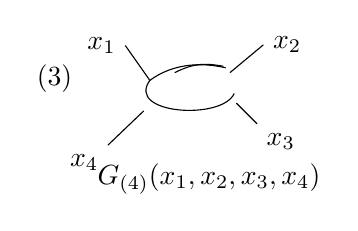
\begin{tikzpicture}[x=1cm,y=1cm,line cap=round]
\node at (-1.66,.17) {\((3)\)};
\draw (-.45,.15)..controls (-.76,-.28) and (.46,-.36)..(.62,-.02);
\draw (-.45,.15)..controls (-.15,.37) and (.21,.38)..(.51,.31);
\draw (-.13,.25)..controls (.11,.37) and (.25,.37)..(.48,.33);
\draw (-.45,.15)--(-.76,.59) node[left] {\(x_1\)};
\draw (.57,.25)--(.99,.60) node[right] {\(x_2\)};
\draw (.65,-.14)--(.91,-.40) node[below right] {\(x_3\)};
\draw (-.53,-.24)--(-.98,-.67) node[below left] {\(x_4\)};
\node at (.30,-1.10) {\(G_{(4)}(x_1,x_2,x_3,x_4)\)};
\end{tikzpicture}}\endgroup}
\end{GelfandAdjacentEvidence}
\begin{GelfandAdjacentEvidence}{GELFAND-P000806}{6}


\SourceFigure{GELFAND-P000806}{green-transform}{%
\par\begingroup\color{black}\GelfandFitDiagram{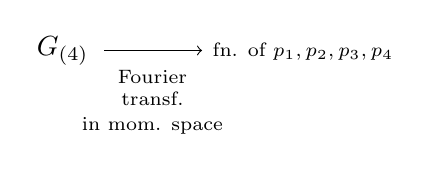
\begin{tikzpicture}[x=1cm,y=1cm]
\node[left] at (0,.12) {\(G_{(4)}\)};
\draw[->] (.08,.13)--(1.32,.13);
\node[align=center,font=\scriptsize] at (.69,-.34) {Fourier\\transf.};
\node[right,align=left,font=\scriptsize] at (1.33,.11)
{\uwave{fn. of \(p_1,p_2,p_3,p_4\)}};
\node[font=\scriptsize] at (.69,-.83) {in mom. space};
\end{tikzpicture}}\endgroup}
\end{GelfandAdjacentEvidence}
\begin{GelfandAdjacentEvidence}{GELFAND-P000806}{7}


(\(\sim\) scattering of \(4\) particles)

Pole \(=\) [\sout{\ldots}] \(m_c^2\)
\Unclear{GELFAND-P000806}{pole-cancellation}{The whole crossed-out expression before \(m_c^2\) is illegible. Its initial strokes may belong to \(m_0\).}
\end{GelfandAdjacentEvidence}


\uwave{fn. \((3)\)} depends only on \(p_j^2\) and \(p_i\cdot p_j\)
(by Lorentz invariance)

and contains \(\delta(p_1+p_2-p_3-p_4)\) (by momentum conservation)

Vertex Green fn.:
\begin{equation*}
\Gamma=\frac{G(p_1,p_2,p_3,p_4)}{G(p_1)G(p_2)\ldots G(p_4)}
\tag{4}
\end{equation*}
(after factoring out the \(\delta\)-fn.)

By perturbation theory (with \(\lambda_0=0\)) we obtain
\begin{equation*}
G^0(p)=\frac{1}{p^2+m^2}.
\tag{5}
\end{equation*}


\Needspace{7\baselineskip}
\begin{GelfandAdjacentEvidence}{GELFAND-P000807}{1}
\SourcePage{GELFAND-P000807}{38}

[crossed out: \sout{\ldots}]
\[
\frac{[G(p_1)\ldots G(p_4)]^{1/2}}{[G^0(p_1)\quad G^0(p_4)]^{1/2}}
\]
\Incomplete{GELFAND-P000807}{top-cancellation}{A heavily crossed-out entry before the upper fraction may read \(\Gamma(p)\). The strokes inside the parentheses are indistinct.}
\end{GelfandAdjacentEvidence}
\begin{GelfandAdjacentEvidence}{GELFAND-P000807}{2}


\[
\lambda(p_i))=\lambda_0\Gamma(p_i))
\frac{[\prod_1^4G(p_i]^{1/2}}{[\prod_1^4G_0(p_i)]^{1/2}}
\quad\text{--- \underline{charge} (invariant)}
\]
\Unclear{GELFAND-P000807}{lambda-arguments}{The arguments of \(\lambda\) and \(\Gamma\) are provisionally read as \(p_i\) with two closing-parenthesis strokes. In the numerator a square bracket follows \(p_i\) with no separate closing parenthesis visible.}
\end{GelfandAdjacentEvidence}
\begin{GelfandAdjacentEvidence}{GELFAND-P000807}{3}

\[
p=(p_1,p_2,p_3,p_4)
\]
\(\lambda_0\) is chosen so that the phys. charge is finite (and all the Green fns. too)

The paradox of \uwave{Landau and Pomeranchuk}:
if we set perturb. theory aside and keep the leading \(\ln\), then we get
\[
\lambda_\mu=\frac{\lambda_0}{1+\frac{3}{2}\frac{\lambda_0}{16\pi^2}
\ \text{\sout{\ldots}}\ \ln\frac{\Lambda}{\mu^2}}.
\]
\Incomplete{GELFAND-P000807}{denominator-cancellation}{The entry before \(\ln\) is heavily crossed out. Its symbols are indistinct.}
\end{GelfandAdjacentEvidence}
\begin{GelfandAdjacentEvidence}{GELFAND-P000807}{4}


[to the right of the formula:] \(\mu\) --- defining point: \(p_ip_j=\mu^2\), \(p_i^2=(\ldots)\mu^2\).

\((\cdot)\) from \((\sum p_i)^2=0\).

\[
\lambda_0>0\quad\Rightarrow\quad\lambda_\mu\longrightarrow\infty
\quad\text{as }\Lambda\longrightarrow\infty
\quad\text{(i.e. the cutoff is removed).}
\]
\Unclear{GELFAND-P000807}{landau-limit}{The fraction has a plus sign after \(1\). Below, \(\lambda_\mu\to\infty\) is written for \(\Lambda\to\infty\).}
\end{GelfandAdjacentEvidence}
\begin{GelfandAdjacentEvidence}{GELFAND-P000807}{5}


The same in quant. electrodyn. [\sout{\ldots}]
(for no bare \(\lambda_0\) does one obtain \(\frac{1}{137}\))
\Incomplete{GELFAND-P000807}{electrodynamics-cancellation}{Diagonal strokes cross out an entry between “electrodyn.” and the opening parenthesis. It is illegible.}
\end{GelfandAdjacentEvidence}


One needs the asymptotics of the coeffs. of the perturbation series arising for
\[
\psi=\frac{d\lambda_\mu}{d\ln\frac{\Lambda}{\mu^2}}
=a_2\lambda_\mu^2+a_3\lambda_\mu^3+\ldots
\]
the asympt. in \(k\) as \(k\to+\infty\) exists

The first 4 have been found explicitly.

\uwave{Idea:} Laplace’s method for the continuum integral

\uline{Sobolev inequality:}
\[
\left[\int(\partial_\sigma\varphi)^2\,d^4x\right]^2
\geq\frac{32\pi^2}{3}\int\varphi^4(x)\,d^4x
\]
equality is attained at
\[
\varphi=\frac{c_1}{(x-x_0)^2+\lambda^2}
\]

[\underline{\underline{Zakharov’s insertion}}\quad
\uwave{\(\Delta\varphi+\varphi^3=0\)}
--- obtained from the Y.–M. eqns.]


\Needspace{7\baselineskip}
\begin{GelfandAdjacentEvidence}{GELFAND-P000808}{1}
\SourcePage{GELFAND-P000808}{unlabelled}

\underline{4.12.78}\qquad \uwave{Gelfand Sem.}

\underline{\underline{A. Guichardet}}

\underline{\underline{Extensions of reps. of top. groups.}}

1. \uwave{Exts. of modules over discr. groups}.

\(E,F\) --- 2 \(G\) modules.
\Unclear{GELFAND-P000808}{module-count}{The heavily retraced digit between the dash and \(G\) provisionally reads 2.}
\end{GelfandAdjacentEvidence}
\begin{GelfandAdjacentEvidence}{GELFAND-P000808}{2}


An ext. of \(E\) by \(F\) --- is a third \(G\)-module \(H\), such that
\(H\supset F\) and \(H/F\cong E\) or an exact seq.
\begin{equation*}
0\longrightarrow F\longrightarrow H\longrightarrow E\longrightarrow0
\tag{1}
\end{equation*}
2 exts. are equiv. if \(\exists\) an isom. such that the diag. commutes.

\SourceFigure{GELFAND-P000808}{equivalence-diagram}{%
\par\begingroup\color{black}\GelfandFitDiagram{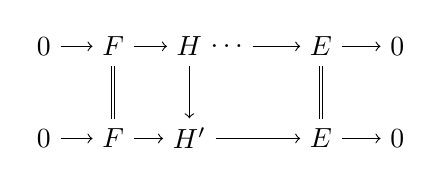
\begin{tikzpicture}[x=.88cm,y=.78cm]
\node (z) at (0,1) {\(0\)};
\node (f) at (1,1) {\(F\)};
\node (h) at (2.1,1) {\(H\)};
\node (cancel) at (2.64,1) {\sout{\(\ldots\)}};
\node (e) at (4,1) {\(E\)};
\node (end) at (5.1,1) {\(0\)};
\node (zb) at (0,-.5) {\(0\)};
\node (fb) at (1,-.5) {\(F\)};
\node (hb) at (2.1,-.5) {\(H'\)};
\node (eb) at (4,-.5) {\(E\)};
\node (endb) at (5.1,-.5) {\(0\)};
\draw[->] (z)--(f);
\draw[->] (f)--(h);
\draw[->] (cancel.east)--(e);
\draw[->] (e)--(end);
\draw[->] (zb)--(fb);
\draw[->] (fb)--(hb);
\draw[->] (hb)--(eb);
\draw[->] (eb)--(endb);
\draw[double] (f.south)--(fb.north);
\draw[->] (h.south)--(hb.north);
\draw[double] (e.south)--(eb.north);
\end{tikzpicture}}\endgroup
\par An entry immediately to the right of the upper \(H\) is crossed out. It may be another \(H\).}
\end{GelfandAdjacentEvidence}
\begin{GelfandAdjacentEvidence}{GELFAND-P000808}{3}


Trivial extension:
\begin{center}
\uwave{\(H=F\oplus E\)}
\end{center}

\uwave{Strong extension:} \((1)\) --- is strong if \(\exists\) a section
[\sout{\(E\xrightarrow{s}H\)}]
\Unclear{GELFAND-P000808}{section-cancel}{The crossed-out arrow is provisionally read as \(E\xrightarrow{s}H\). Diagonal strokes cross the right-hand letter.}
\end{GelfandAdjacentEvidence}
\begin{GelfandAdjacentEvidence}{GELFAND-P000808}{4}


\SourceFigure{GELFAND-P000808}{section-diagram}{%
\par\begingroup\color{black}\GelfandFitDiagram{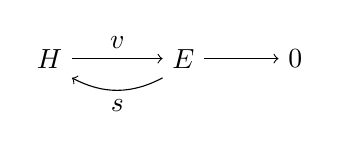
\begin{tikzpicture}[x=1cm,y=1cm]
\node (h) at (0,0) {\(H\)};
\node (e) at (1.7,0) {\(E\)};
\node (z) at (3.12,0) {\(0\)};
\draw[->] (h)--node[above] {\(v\)}(e);
\draw[->] (e)--(z);
\draw[->] (e.south west) to[bend left=28] node[below] {\(s\)} (h.south east);
\end{tikzpicture}}\endgroup}
\end{GelfandAdjacentEvidence}
\begin{GelfandAdjacentEvidence}{GELFAND-P000808}{5}


\uwave{\(v\cdot s=\mathrm{id}\)};
\uwave{\(s\) --- a morphism of groups} (and not of \uwave{\(G\)-modules})
\Unclear{GELFAND-P000808}{projection-symbol}{The sign in \(v\cdot s=\mathrm{id}\) and over the arrow provisionally reads \(v\).}
\end{GelfandAdjacentEvidence}


[inserted below “groups”: (abelian).]

(if \(s\) --- a morph. of \(G\)-mods., the extension is trivial)

Set of equiv. classes of [inserted above the line: strong] extensions:
\uwave{\(\operatorname{Ext}^1(E,F)\)}

Method: cohomology

\(\operatorname{Hom}(E,F)\) --- morph. of groups

this is a \(G\)-module. The action is given by
\[
gu=g\cdot u\cdot g^{-1}
\]


\Needspace{7\baselineskip}
\begin{GelfandAdjacentEvidence}{GELFAND-P000809}{1}
\SourcePage{GELFAND-P000809}{43}

\underline{\underline{Def.}}
\[
H^1(G,\operatorname{Hom}(E,F))
\]
\uwave{1-cocycles}
\[
f:G\longrightarrow\operatorname{Hom}(E,F)
\]
\begin{equation*}
f(gg')=f(g)+g\circ f(g')\circ g^{-1}.
\tag{2}
\end{equation*}
\Unclear{GELFAND-P000809}{cocycle-g-strokes}{The lower loop of the first \(g\) after the plus sign in (2) is retraced. It reads \(g\), with an indistinct adjoining stroke.}
\end{GelfandAdjacentEvidence}
\begin{GelfandAdjacentEvidence}{GELFAND-P000809}{2}


\(Z^1\) --- all cocycles.

1-coboundaries (\(B^1\)).
\[
\exists\,u\in\operatorname{Hom}(E,F):\quad
f(g)=g\circ u\circ g^{-1}-u
\]
\[
H^1\underset{\mathrm{def}}{=}Z^1/B^1.
\]
There is a correspondence (one-to-one)
\[
H^1\cong\operatorname{Ext}^1(E,F)
\]
From the cocycle \(\varphi\) construct an extension:
\[
H=F\oplus E
\]
\begin{equation*}
g(f,e)=(gf+\varphi(g)g\cdot e,\quad g\cdot e).
\tag{3}
\end{equation*}
or in matrices:
\[
\begin{pmatrix}
V_g&\varphi(g)U_g\\
0&U_g
\end{pmatrix}
\quad\text{--- \uwave{this is how the action is constructed}.}
\]
\Unclear{GELFAND-P000809}{group-block-glyphs}{The last letter at the top right is provisionally read as \(U_g\), as on the diagonal. The lower-left sign is open at the right and provisionally reads \(0\).}
\end{GelfandAdjacentEvidence}
\begin{GelfandAdjacentEvidence}{GELFAND-P000809}{3}


\(V_g,U_g\) --- [\sout{\ldots}] reps. of \(G\) in the corresp. spaces.
\Unclear{GELFAND-P000809}{representation-count}{An overwritten or crossed-out entry before “reps.” may be the numeral 2.}
\end{GelfandAdjacentEvidence}
\begin{GelfandAdjacentEvidence}{GELFAND-P000809}{4}


From this one can obtain the def. of a cocycle.

2 reps. equiv. \(\Longleftrightarrow\) the cocycles are homologous

2. \uwave{Extensions of modules over Lie algebras}.

[on the right:]
\[
X\longrightarrow\begin{pmatrix}A(X)&f(X)\\0&B(X)\end{pmatrix}
\]
\Unclear{GELFAND-P000809}{lie-block-glyphs}{The retraced letter at the top right provisionally reads \(f\). The lower-left sign is open at the right and is rendered as \(0\).}
\end{GelfandAdjacentEvidence}


a cocycle is a linear map \(f:\mathfrak g\longrightarrow\operatorname{Hom}(E,F)\)

\uwave{the def. of a cocycle} has the form:
\begin{equation*}
f([X,Y])=X\circ f(Y)-f(Y)\circ X-Y\circ f(X)+f(X)\circ Y.
\tag{4}
\end{equation*}
\(f\) --- a coboundary if \(\exists\,u\)
\begin{equation*}
f(X)=X\circ u-u\circ X.
\tag{5}
\end{equation*}

\underline{Lemma} 1. \(E,F\) have [inserted above the line: distinct]
infinitesim. characters \(\Rightarrow\)
\[
\Rightarrow\quad\operatorname{Ext}^1(E,F)=0
\]
\(\mathfrak g\longmapsto U(\mathfrak g)\)\qquad
univ. enveloping algebra, \(Z(\mathfrak g)\) --- its center


\Needspace{7\baselineskip}
\begin{GelfandAdjacentEvidence}{GELFAND-P000810}{1}
\SourcePage{GELFAND-P000810}{unlabelled}
Let \(\underline{\underline{u\in Z(\mathfrak g)}}\) act in \(E\) by mult. by a scalar
\[
\text{\uwave{\(\displaystyle u\cdot e=\chi(u)e\)}}
\]
Then \(\chi\in\operatorname{Hom}(Z(\mathfrak g),\mathbb C)\)

\uwave{this is an infinitesim. character.}

\(H^1(\mathfrak g,\operatorname{Hom}(E,F))\) — \uwave{is}

\(H^1(\mathfrak g,\mathfrak h,\operatorname{Hom}(E,F))\),\qquad
\(\mathfrak h\subset\mathfrak g\)

[In the right margin: \(\ldots\).]
\Unclear{GELFAND-P000810}{right-margin-mark}{Isolated illegible mark}
\end{GelfandAdjacentEvidence}
\begin{GelfandAdjacentEvidence}{GELFAND-P000810}{2}


(describes extensions trivial from the point of view of \(\mathfrak h\)).
\[
Z^1(\mathfrak g,\mathfrak h,\operatorname{Hom}(E,F))
=\{f\in Z^1(\mathfrak g,\ldots),\quad f|_{\mathfrak h}=0\}
\]
\[
H^1(\mathfrak g,\mathfrak h,\ldots)\in H^1(\mathfrak g,\ldots)
\]
\Unclear{GELFAND-P000810}{relative-relation}{The manuscript places the sign \(\in\) between the groups.}
\end{GelfandAdjacentEvidence}
\begin{GelfandAdjacentEvidence}{GELFAND-P000810}{3}


\uline{Comments}:

\uwave{One can use the differential}:
\[
(df)(x,y)=f([x,y])-xf(y)+yf(x)
\]
\(xf(y)\) — \uuline{action} Lie alg.

(above, written using the \uwave{commutator})

3. \uwave{Extensions of modules over Lie groups}.

\(G\)-module — top. vect. space, \(G\) acts continuously.

\(\mathfrak g\) — Lie alg.

\(\begin{array}{@{}l@{}} K\subset G\\[-3pt] \vert\\[-3pt]\text{max. comp. subgp.},\end{array}\)

\(\mathfrak k\) — corresp. alg.,

\(E,F\) — t.v.s.

\uwave{1st idea.}\quad \uwave{cocycles}
\[
f:G\longrightarrow\operatorname{Hom}(E,F)
\]
\((e,g)\longmapsto f(g)e\)\qquad cont. in \(g\) and \(e\).

\uwave{2nd idea}: in place of \(E,F\) — the space of diff. vectors \(E_\infty,F_\infty\)

good, but imperfect when \(\underline{\underline{E=\mathbb C}}\). Suppose so.
\Unclear{GELFAND-P000810}{differentiable-vectors-phrase}{The manuscript leaves the sense of “imperfect” unspecified.}
\end{GelfandAdjacentEvidence}
\begin{GelfandAdjacentEvidence}{GELFAND-P000810}{4}


\uline{Theorem}:
\SourceFigure{GELFAND-P000810}{theorem-attributions}{%
\par\begingroup\color{black}\GelfandFitDiagram{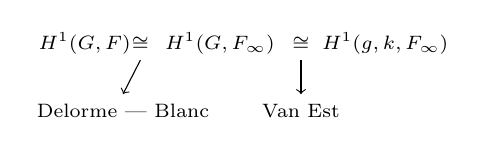
\begin{tikzpicture}[x=1cm,y=.85cm, every node/.style={font=\scriptsize}]
\node[anchor=west,inner sep=0] at (0,0) {\(H^1(G,F)\)};
\node (a) at (1.30,0) {\(\cong\)};
\node[inner sep=0] at (2.31,0) {\(H^1(G,F_\infty)\)};
\node (b) at (3.34,0) {\(\cong\)};
\node[anchor=west,inner sep=0] at (3.60,0) {\(H^1(\mathfrak g,\mathfrak k,F_\infty)\)};
\node (db) at (1.08,-1) {Delorme — Blanc};
\node (ve) at (3.34,-1) {Van Est};
\draw[->] (a.south) -- (db.north);
\draw[->] (b.south) -- (ve.north);
\end{tikzpicture}}\endgroup\par}
\end{GelfandAdjacentEvidence}
\begin{GelfandAdjacentEvidence}{GELFAND-P000810}{5}

\Unclear{GELFAND-P000810}{theorem-arrows}{The first algebra symbol in the right-hand group is retraced and provisionally reads \(\mathfrak g\).}
\end{GelfandAdjacentEvidence}
\begin{GelfandAdjacentEvidence}{GELFAND-P000810}{6}


\uwave{For \(\mathbb R\) nontriv.}
\[
\begin{pmatrix}1&at\\0&1\end{pmatrix}
\]
— \uwave{an extension} of the triv. \(\mathbb R\)-module by the trivial one

there are no corresp. reps. of groups and algebras

(\uwave{in cohom.}: one must take cohom. triv.
[crossed out: \(\ldots\)] on the compact subgroup).
\Incomplete{GELFAND-P000810}{bottom-cancellation}{word obscured by strokes}
\end{GelfandAdjacentEvidence}



\Needspace{7\baselineskip}
\begin{GelfandAdjacentEvidence}{GELFAND-P000811}{1}
\SourcePage{GELFAND-P000811}{44}
\uwave{Imperfection}:

even if \(F\) — an irred. unit. rep., then it may be that
\[
\underline{\dim H^1(G,F)\mathrel{\overset{?}{=}}+\infty}
\]
\Unclear{GELFAND-P000811}{dimension-sign}{The sign has two nearly horizontal strokes with a superimposed angle. Its shape could be \(\geq\). Equality agrees with the following example.}
\end{GelfandAdjacentEvidence}
\begin{GelfandAdjacentEvidence}{GELFAND-P000811}{2}


\uline{Example}\qquad \(G\) — the aff. group of the line\quad
\quad \(ax+b\)
\Unclear{GELFAND-P000811}{affine-mark}{The mark resembles \(R\), with some strokes possibly crossing it out.}
\end{GelfandAdjacentEvidence}
\begin{GelfandAdjacentEvidence}{GELFAND-P000811}{3}


\(B^1\) is everywhere dense in \(Z^1\), but \(\underline{\underline{\dim Z^1/B^1=+\infty}}\)

Reason: \(F\) weakly contains the trivial rep.

For semisimple groups all is well,
[crossed out: \(\ldots\)]
\Incomplete{GELFAND-P000811}{semisimple-cancellation}{the original signs are illegible}
\end{GelfandAdjacentEvidence}
\begin{GelfandAdjacentEvidence}{GELFAND-P000811}{4}


Let \(G\) — semisimple;

\uwave{unit. irred. rep}.

It is known when \(H^1=0\).

For nonsemisimple groups:
\[
\text{\uwave{\(\displaystyle SO_0(m,n)\)}}
\]
there are no nonunit. reps. with nonzero cohom.

\Unclear{GELFAND-P000811}{nonsemisimple-context}{The manuscript gives the heading “For nonsemisimple groups” and the abbreviation “nonunit.” alongside \(SO_0(m,n)\).}
\end{GelfandAdjacentEvidence}
\begin{GelfandAdjacentEvidence}{GELFAND-P000811}{5}


\uwave{Add. drawback of the 1st idea}.

The lemma about infinitesim. char. is false!

There is a counterexample [crossed out: \(\ldots\)] for \(SL(2,\mathbb R)\)
\Unclear{GELFAND-P000811}{counterexample-cancellation}{Possibly “all”, with several letters obscured by transverse strokes.}
\end{GelfandAdjacentEvidence}
\begin{GelfandAdjacentEvidence}{GELFAND-P000811}{6}


\uwave{2nd idea}: the lemma about infinitesim. chars. is true, but

[In the left margin, crossed out: \(\ldots\)]
\Unclear{GELFAND-P000811}{second-margin-cancellation}{Possibly a repeated “but”.}
\end{GelfandAdjacentEvidence}
\begin{GelfandAdjacentEvidence}{GELFAND-P000811}{7}

\[
H^1(G,\operatorname{Hom}(E_\infty,F_\infty))
\]
is hard to compute.

\[
L_\infty^2\longrightarrow L_\infty^2
\]
[To the left and on the next line, crossed out: \sout{\(L_\infty^2\longrightarrow\ldots\)};\quad
\sout{Problem \(\ldots\)}]
\Incomplete{GELFAND-P000811}{long-cancellations}{The start of the upper entry provisionally reads \(L_\infty^2\) and an arrow is visible farther right. In the lower line, strokes obscure the words and signs following “Problem”.}
\end{GelfandAdjacentEvidence}
\begin{GelfandAdjacentEvidence}{GELFAND-P000811}{8}


\uline{3rd idea}.
\[
E,F\rightsquigarrow E_K,F_K
\]
(vectors incl. in finite-dimensional reps. of \(K\)).

\Incomplete{GELFAND-P000811}{k-cancellations}{Two text fragments are crossed out. Isolated loops are visible, with the words obscured.}
\end{GelfandAdjacentEvidence}
\begin{GelfandAdjacentEvidence}{GELFAND-P000811}{9}


\(K\)-finite;\qquad \uwave{\(K\) — max. comp. subgroup}

\(SL(2,\mathbb R)\) — for all irred. Harish-Chandra modules one can compute
\Unclear{GELFAND-P000811}{hc-abbreviation}{The abbreviation «непр.» is provisionally expanded as “irreducible”.}
\end{GelfandAdjacentEvidence}
\begin{GelfandAdjacentEvidence}{GELFAND-P000811}{10}

\[
H^1(\mathfrak g,\mathfrak k,\operatorname{Hom}(E_K,F_K))
\]
algebra without topology.

4. \uwave{The case of a semidirect product}.
\[
G=B\underset{\text{semidir.}}{\times}A\underset{\sigma}{=}B\wedge A,
\qquad B=\mathbb R^n,\quad A\text{ — Lie group}
\]
\Unclear{GELFAND-P000811}{product-equality-mark}{The sign below the equality provisionally reads \(\sigma\), possibly \(g\). The sign between \(B\) and \(A\) is \(\wedge\).}
\end{GelfandAdjacentEvidence}


(e.g., the aff. group of the line).

\(B^*\) — dual space,\qquad \(\langle b,x\rangle\) — duality.

\(X=A\)-orbit in \(B^*\)

(the action of \(A\) in \(B\) is precisely the def. of the semidirect prod.)


\Needspace{7\baselineskip}
\begin{GelfandAdjacentEvidence}{GELFAND-P000812}{1}
\SourcePage{GELFAND-P000812}{unlabelled}
[To the left of the date, crossed out: \(\ldots\).]
\Incomplete{GELFAND-P000812}{date-cancellation}{the word or digits are illegible}
\end{GelfandAdjacentEvidence}
\begin{GelfandAdjacentEvidence}{GELFAND-P000812}{2}


\uuline{12/II-79 }\qquad \uline{Gelfand Sem.}

\uwave{What does one need to know?} (according to \uline{A. A. Belavin}):

I.\quad \uline{Feynman}.

\hspace{1em}1.\quad Course for housewives, chs. 8, 9.

\hspace{1em}2.\quad Statistical physics

\hspace{1em}3.\quad Path integrals (with Gibbs)
\Unclear{GELFAND-P000812}{feynman-coauthor}{The manuscript reads «Гиббсом» (Gibbs). The probable reference is to A. R. Hibbs, Feynman’s coauthor on path integrals.}
\end{GelfandAdjacentEvidence}
\begin{GelfandAdjacentEvidence}{GELFAND-P000812}{3}


\(\overline{\underline{\mathrm{II}}}\).\quad \uline{Huang} “Statist. Mechanics” Chapter: Onsager’s solution.

\(\overline{\underline{\mathrm{III}}}\).\quad \uline{F. Klein} “Lectures on the History of Mathematics in the \uuline{XIX} Century”

[Crossed-out number: \(\ldots\)]
\Unclear{GELFAND-P000812}{list-cancellation}{possibly IV}
\end{GelfandAdjacentEvidence}
\begin{GelfandAdjacentEvidence}{GELFAND-P000812}{4}

[4. The little books with blue cubes on the cover (against a white background)

\hspace{1em}(Feynman: “Fund. Laws of Physics”).]

\SourceFigure{GELFAND-P000812}{list-placement-arrow}{%
\par\begingroup\color{black}\GelfandFitDiagram{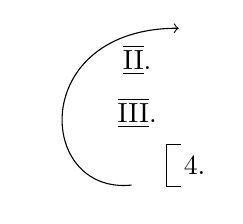
\begin{tikzpicture}[x=.8cm,y=.83cm]
\draw[->] (1.12,0) .. controls (-.4,-.15) and (-.52,2.4) .. (1.87,2.4);
\node at (1.21,1.91) {\(\overline{\underline{\mathrm{II}}}\).};
\node at (1.21,1.10) {\(\overline{\underline{\mathrm{III}}}\).};
\draw (1.9,.62) -- (1.67,.62) -- (1.67,-.02) -- (1.9,-.02);
\node at (2.12,.3) {4.};
\end{tikzpicture}}\endgroup\par
The arrow in the left margin runs from the crossed-out numeral to the space before II.}
\end{GelfandAdjacentEvidence}
\begin{GelfandAdjacentEvidence}{GELFAND-P000812}{5}


\(\overline{\underline{\mathrm{IV}}}\).\quad \uline{Dirac} Article in the book “Dirac’s Monopole”

\hspace{1em}books. “Lectures on Quantum Mechanics”

\hspace{1em}“[ditto marks for ‘Lectures on’] Field Theory”

\hspace{1em}“General Relativity”

\(\overline{\underline{\mathrm{V}}}\).\quad \uline{Akhiezer}, \uline{Berestetskii} “Quantum Electrodynamics”

\hspace{1em}(one should know the contents, but needn’t read it)

\(\overline{\underline{\mathrm{VI}}}\).\quad Collection “Particles and Compensating Fields”, Article by \uwave{Yang and Mills}.

\(\overline{\underline{\mathrm{VII}}}\).\quad \uline{Konopleva}, \uline{Popov}: “Gauge Fields” (the part written by Popov)

\uline{Belavin}

Problem put fwd. for a competition by the Chernogolovka Royal Phys. Soc.: or

What remains unsolv. about instantons?

\(A,B\) — 2 quaternionic matrices \(N\times(N+1)\)

One must find a parametrization [inserted above the line: “of such”] of pairs of matrices \(A\) and \(B\), such that
if \(M=xA+B\), then \(MM^+\) is real (for every quaternion \(x\)),
up to the group action
\[
GMV
\]
\[
\begin{aligned}
G&\qquad N\times N\\
V&\qquad (N+1)\times(N+1)\qquad VV^+=1
\end{aligned}
\]
\Unclear{GELFAND-P000812}{group-letter}{The same handwritten symbol is provisionally set as \(V\) throughout. Its shape could also be \(U\) or \(\upsilon\).}
\end{GelfandAdjacentEvidence}
\begin{GelfandAdjacentEvidence}{GELFAND-P000812}{6}


There should be \(8N-3\) parameters in all.

One must find a beautiful parametrization of such matrices.

\uwave{On some exactly solvable 2-dimensional QFT problems}.

A naive argument about \uwave{non-escape}. (Wilson)
\[
\psi(x)\qquad S[\psi,\ldots]\text{ — action},
\qquad \delta S=0\text{ — eqs. of motion}
\]
\[
\psi(x)\longrightarrow e^{i\alpha(x)}\psi(x)
\qquad\text{— gauge invariance}
\]
\Unclear{GELFAND-P000812}{final-argument}{On the left of the formula, \(x\) is written over earlier strokes. The original sign is illegible.}
\end{GelfandAdjacentEvidence}



\Needspace{7\baselineskip}
\begin{GelfandAdjacentEvidence}{GELFAND-P000813}{1}
\SourcePage{GELFAND-P000813}{63}
\[
\langle\psi(x)\overline{\psi(y)}\rangle
=e^{i(\alpha(x)-\alpha(y))}\langle\ldots\rangle
\]
\(\Rightarrow\) correl. fns. \(0\) \(\Rightarrow\) impossibility
[crossed out: \(\ldots\)] for charged objects.
\Incomplete{GELFAND-P000813}{correlation-cancellation}{letters obscured by strokes}
\end{GelfandAdjacentEvidence}
\begin{GelfandAdjacentEvidence}{GELFAND-P000813}{2}


\uwave{Talk on hidden symmetry}.

Passing from a cont. int. to a finite multiple integral can break the symmetry.

1) There is a theory
\[
\Box\varphi=\sin\varphi,\qquad \varphi(x,t),\qquad
\Box=\frac{\partial^2}{\partial t^2}-\frac{\partial^2}{\partial x^2}
\]
a quasiclass. spectrum has been obtained.

2) Next, there is a Ham. (\uline{Baxter}):
\begin{equation*}
H=\sum_{n=1}^N\sum_{\alpha=1}^3 J_\alpha\sigma_n^\alpha\sigma_{n+1}^\alpha \tag{1}
\end{equation*}

\SourceFigure{GELFAND-P000813}{spin-chain-sites}{%
\par\begingroup\color{black}\GelfandFitDiagram{\begin{tikzpicture}[x=1cm,y=1cm]
\draw[thick] (0,0) circle[radius=.045cm];
\foreach \x in {.55,1.2,1.83,2.35,2.94,4.03}
  \draw (\x,0) circle[radius=.032cm];
\node at (.15,-.30) {\(1\)};
\node at (.57,-.30) {\(2\)};
\node at (1.30,-.30) {\(3\)};
\node at (1.85,-.30) {\(\cdot\)};
\node at (2.23,-.30) {\(\cdot\)};
\node at (4.16,-.30) {\(N\)};
\end{tikzpicture}}\endgroup\par}
\end{GelfandAdjacentEvidence}
\begin{GelfandAdjacentEvidence}{GELFAND-P000813}{3}


\[
\begin{gathered}
\sigma_n^\alpha=1\otimes1\otimes\ldots\otimes
\sigma^\alpha\otimes1\otimes\ldots\otimes1.\\
\alpha=1,2,3
\end{gathered}
\]
\Unclear{GELFAND-P000813}{sigma-site}{Below \(\sigma^\alpha\) is a crossed-out mark, possibly \(n\).}
\end{GelfandAdjacentEvidence}
\begin{GelfandAdjacentEvidence}{GELFAND-P000813}{4}


[On the right] (1-dimensional quant. chain)

\(\boxed{N+1=1}\) — periodicity condition.
\[
\begin{gathered}
\sigma^3=\begin{pmatrix}1&0\\0&-1\end{pmatrix},\quad
\sigma^1=\begin{pmatrix}0&1\\1&0\end{pmatrix},\quad
\sigma^2=\begin{pmatrix}0&-i\\i&0\end{pmatrix};\qquad J_\alpha\in\mathbb R
\end{gathered}
\]
\(H\) — a matrix \(2^N\times2^N\)

\uline{Problem}: find the eigenvecs. and eigenvalues.

In meaning, these models are analogous to 4-dim. gauge theories.

In the limit, 2) yields \(\sin\)-Gordon.

Baxter solved syst. (1)

The Hamiltonian itself is Heisenberg’s. (anisotropic, because of \(J_\alpha\) — Heisenberg ferromagnet)

(or \(XYZ\) model)

Luther reduced (1) to the Thirring model.

The relations hold:
\begin{equation*}
\begin{cases}
[\sigma_n^\alpha,\sigma_m^\beta]=0,\qquad n\ne m\\
[\sigma_n^\alpha,\sigma_n^\beta]=\varepsilon_{\alpha\beta\gamma}\,\sigma_n^\gamma\\
[\sigma_n^1,\sigma_n^2]_+=0
\end{cases}\tag{2}
\end{equation*}
\([\, ,\,]_+\) — anticommutator

\Unclear{GELFAND-P000813}{commutator-normalization}{The middle line of (2) shows no factor before \(\varepsilon_{\alpha\beta\gamma}\).}
\end{GelfandAdjacentEvidence}
\begin{GelfandAdjacentEvidence}{GELFAND-P000813}{5}


Let us make lattice fermions.
\begin{equation*}
\psi_n^\pm=(\sigma_n^1\pm i\sigma_n^2)\prod_{m=1}^{n-1}\sigma_m^3;\tag{3}
\end{equation*}
these are fermions, i.e.
\begin{equation*}
\begin{cases}
[\psi_n^+,\psi_m^+]_+=0\\
[\psi_n^-,\psi_m^+]_+=\delta_{nm}
\end{cases}\tag{4}
\end{equation*}
\Unclear{GELFAND-P000813}{fermion-normalization}{In (3) there is no factor before the parentheses. In (4) the right-hand side is \(\delta_{nm}\).}
\end{GelfandAdjacentEvidence}
\begin{GelfandAdjacentEvidence}{GELFAND-P000813}{6}


In [crossed out: \(\ldots\)] fact — this is how Onsager solved the Ising model:
\Incomplete{GELFAND-P000813}{bottom-cancellation}{the word is obscured by strokes}
\end{GelfandAdjacentEvidence}


express \(\sigma\) in terms of \(\psi\): \(H\) will become quadr. and everything is diagonalized


\Needspace{7\baselineskip}
\begin{GelfandAdjacentEvidence}{GELFAND-P000814}{1}
\SourcePage{GELFAND-P000814}{unlabelled}
Let us take a Fourier transf.
\begin{equation*}
\widetilde\psi_k^\pm=\sum_n\psi_n^\pm e^{ikn}\tag{5}
\end{equation*}
[crossed out: \(\ldots\)]
\Unclear{GELFAND-P000814}{assertion-cancellation}{Possibly “I will formulate” or “we will formulate”. Cancellation strokes obscure the ending.}
\end{GelfandAdjacentEvidence}
\begin{GelfandAdjacentEvidence}{GELFAND-P000814}{2}

\uline{Assertion}.
\begin{equation*}
H=\sum_n(\sigma_n^1\sigma_{n+1}^1+\Delta\sigma_n^3),\qquad
\Delta\text{ — a number}\tag{6}
\end{equation*}
\begin{equation*}
\dot\sigma_n(t)=i[\sigma_n,H]\tag{7}
\end{equation*}
— eqs. of motion; for the solutions \(\forall t\) the commut. rels. hold (2)
\[
\sigma_n(0)=\sigma_n.
\]
After substitution the eqs. become linear (in \(\psi\))

\(\Rightarrow\) this is equiv. to finding eigenvectors.

(\(\sigma\) can be expressed in terms of \(\psi\))

We obtain the eqs.
\begin{equation*}
\dot\psi_n=\psi_{n+1}-\psi_{n-1}\tag{8}
\end{equation*}
Expr. for the Hamiltonian \uwave{in the orig. problem}.
\begin{equation*}
H\sim\sum_n\bigl(\psi_n\psi_{n+1}^+-\psi_n^+\psi_{n+1}
+\psi_n^+\psi_n\psi_{n+1}^+\psi_{n+1}\bigr)\tag{9}
\end{equation*}
[crossed out: \sout{\(\sigma_1\) and \(\sigma_2\)}.]
\Unclear{GELFAND-P000814}{sigma-cancellation}{The cancelled symbols provisionally read \(\sigma_1\) and \(\sigma_2\). The indices may be superscripts.}
\end{GelfandAdjacentEvidence}
\begin{GelfandAdjacentEvidence}{GELFAND-P000814}{3}

\(\sigma_n\) is expr. in terms of \(\psi\) by induction.

(9) — Ham. of the lattice Thirring model (already nonlin.)

Passing to the continuous case, we obtain:
\begin{equation*}
\int dx\left[\psi_1^+(x)\frac{\partial\psi_2(x)}{\partial x}
+\psi_1^+\psi_2\psi_1^+\psi_2^+\text{\sout{]}}
+\underset{\substack{\vert\\\text{Hermitian conj.}}}{\text{h.c.}}\right]\tag{10}
\end{equation*}
\Unclear{GELFAND-P000814}{quartic-term}{The subscript on the third factor is retraced and reads \(1\). The first closing bracket is crossed out.}
\end{GelfandAdjacentEvidence}
\begin{GelfandAdjacentEvidence}{GELFAND-P000814}{4}

\[
\underline{x=na},\qquad\psi(x)\approx\psi_n
\]
\(\psi_1,\psi_2\) — from different \uline{even} and \uline{odd} lattice sites

\uline{1975}\qquad \uwave{Mandelstam} and\ldots:
\uline{quant. Thirring model \(\sim\) quant. mod. \(\sin\)-Gordon}

\uline{quant. mod. \(\sin\)-Gord}
\begin{equation*}
\Box\varphi=\sin\varphi\tag{11}
\end{equation*}
\begin{equation*}
[\dot\varphi(t,x),\varphi(t,y)]=\delta(x-y)\tag{12}
\end{equation*}
\Unclear{GELFAND-P000814}{canonical-normalization}{The right-hand side of (12) shows \(\delta(x-y)\) without a factor \(i\).}
\end{GelfandAdjacentEvidence}
\begin{GelfandAdjacentEvidence}{GELFAND-P000814}{5}

\begin{equation*}
\psi=i e^{i\alpha\Phi+\beta\int_{-\infty}^x\dot\Phi(y)\,dy}\tag{13}
\end{equation*}
\Unclear{GELFAND-P000814}{bosonization-notation}{The field in (13) is set as \(\Phi\), possibly \(\varphi\). There is an \(i\) before \(e\) and no additional \(i\) is visible before \(\beta\).}
\end{GelfandAdjacentEvidence}


\(\Downarrow\)\qquad (when \(\alpha\beta=4\pi\))
\begin{equation*}
[\psi(x),\psi^+(y)]_+=\delta(x-y)\tag{14}
\end{equation*}

End of the introduction.

\uwave{Sasha Zamolodchikov}. Zamolodchikov algebra.

[Under the name:] (Moscow)
\[
\underset{\substack{\vert\\\text{symbols}}}{A_i(\theta)},\qquad 1\le i<M
\]


\Needspace{7\baselineskip}
\begin{GelfandAdjacentEvidence}{GELFAND-P000815}{1}
\SourcePage{GELFAND-P000815}{64}
[At the upper left: \(\ldots\)]
\Unclear{GELFAND-P000815}{top-edge-mark}{An isolated short vertical stroke with a rightward hook at its top. Its meaning is unclear.}
\end{GelfandAdjacentEvidence}
\begin{GelfandAdjacentEvidence}{GELFAND-P000815}{2}


One can write products
\begin{equation*}
A_i(\theta_1)A_\alpha(\theta_2)
=S_{ik}^{\alpha\beta}(\theta_1-\theta_2)A_\beta(\theta_2)A_k(\theta_1)\tag{15}
\end{equation*}
\[
1\le\beta<M,\qquad 1\le\alpha<M.
\]
\Unclear{GELFAND-P000815}{index-range}{Both upper bounds in the manuscript use strict \(<\). The example below uses \(A_2\) with \(M=2\).}
\end{GelfandAdjacentEvidence}
\begin{GelfandAdjacentEvidence}{GELFAND-P000815}{3}


[crossed out: \(\ldots\)]
\Incomplete{GELFAND-P000815}{m-cancellation}{the original mark is illegible}
\end{GelfandAdjacentEvidence}
\begin{GelfandAdjacentEvidence}{GELFAND-P000815}{4}

\(\underline{M=2}\)
\begin{equation*}
\begin{cases}
A_1A_1=aA_1A_1+dA_2A_2\\
A_1A_2=bA_2A_1+cA_1A_2
\end{cases}\tag{16}
\end{equation*}
and 2 more rels. obt. by replacing 1 with 2.

This still has to be made compatible with associativity.

\uwave{On \(S\) the corresp. condition is imposed}
\[
\bigl(A_1(\theta_1)A_1(\theta_2)\bigr)A_2(\theta_3)
=A_1(\theta_1)\bigl(A_1(\theta_2)A_2(\theta_3)\bigr)
\]
The eqs. lead to factorization of multiparticle \(S\)-matrices

Thus he found the \(S\)-matrix of \(\sin\)-Gordon etc.

\uwave{The eqs. for} \(a,b,c,d\) (from (16)) \uwave{are solved explicitly} (!)
\begin{equation*}
\begin{cases}
a=\operatorname{sn}(\theta+\eta,k)\\
b=\operatorname{sn}(\theta-\eta,k)\\
c=\operatorname{sn}(2\eta,k)\\
d=k\cdot abc
\end{cases}\tag{17}
\end{equation*}
\Unclear{GELFAND-P000815}{elliptic-parameter}{The second argument of \(\operatorname{sn}\) and the factor in \(d\) are provisionally set as \(k\), possibly \(\kappa\).}
\end{GelfandAdjacentEvidence}
\begin{GelfandAdjacentEvidence}{GELFAND-P000815}{5}


\uline{These are all solns. up to a factor}.

Baxter used such objects
\begin{equation*}
T^{\alpha_1,\beta_1,\ldots,\alpha_N,\beta_N}(\theta)
=S_{i_1i_2}^{\alpha_1\beta_1}S_{i_2i_3}^{\alpha_2\beta_2}
\ldots S_{i_Ni_1}^{\alpha_N\beta_N}\tag{18}
\end{equation*}
The result is a \(2^N\times2^N\) matrix. It turns out that

[To the left of (19) crossed out: \(\ldots\)]
\Incomplete{GELFAND-P000815}{commutator-cancellation}{the original mark is illegible}
\end{GelfandAdjacentEvidence}
\begin{GelfandAdjacentEvidence}{GELFAND-P000815}{6}

\begin{equation*}
[T(\theta),H]=0\tag{19}
\end{equation*}
(\(\Rightarrow\) infin. set of integrals of motion)
\begin{equation*}
[T(\theta_1),T(\theta_2)]=0\tag{20}
\end{equation*}
(\(\Rightarrow\) in involution)

In fact he solved it exactly.

\SourceFigure{GELFAND-P000815}{margin-angle}{%
\par\begingroup\color{black}\GelfandFitDiagram{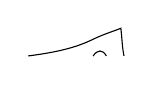
\begin{tikzpicture}[x=.8cm,y=.8cm]
\draw (0,0) .. controls (.46,.06) and (.75,.13) .. (1.02,.26)
  .. controls (1.18,.34) and (1.35,.39) .. (1.47,.44)
  .. controls (1.49,.28) and (1.49,.15) .. (1.52,0);
\draw (1.03,0) .. controls (1.10,.10) and (1.18,.11) .. (1.24,0);
\end{tikzpicture}}\endgroup\par
Angular mark at the lower left. Its strokes end at the same horizontal boundary in the source image. The full shape and purpose are unclear.}
\end{GelfandAdjacentEvidence}



\Needspace{7\baselineskip}
\begin{GelfandAdjacentEvidence}{GELFAND-P000816}{1}
\SourcePage{GELFAND-P000816}{unlabelled}
\uuline{19/II-79}\qquad \uline{Gelfand Sem.}

\uuline{Belavin}.

\[
A_i(\theta),\qquad 1\le i\le M,\qquad\text{— symbols}
\]
\(\theta\) — a parameter

\uwave{Zamolodchikov algebra}.

\begin{equation*}
A_i(\theta_1)A_\alpha(\theta_2)
=S_{ik}^{\alpha\beta}(\theta_1-\theta_2)A_\beta(\theta_2)A_k(\theta_1)\tag{1}
\end{equation*}
Associativity is required too. Then cubic rels. arise.
\[
A_i(\theta_1)A_j(\theta_2)A_k(\theta_3)
\]
[On the right:] (free assoc. algebra gen. by \(M\) continua of vars. with rels.)
\Unclear{GELFAND-P000816}{free-algebra-word}{The marginal phrase reads «континуумами перем.» (continua of vars.).}
\end{GelfandAdjacentEvidence}
\begin{GelfandAdjacentEvidence}{GELFAND-P000816}{2}


Interpretation (physical)

\SourceFigure{GELFAND-P000816}{particle-motion}{%
\par\begingroup\color{black}\GelfandFitDiagram{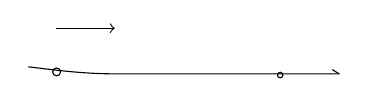
\begin{tikzpicture}[x=1cm,y=1cm]
\draw[->] (.35,.58) -- (1.10,.58);
\draw (0,.09) .. controls (.45,.035) and (.73,0) .. (1.15,0) -- (3.95,0);
\draw (3.86,.055) -- (3.95,0);
\draw (.36,.025) circle[radius=.05cm];
\draw (3.20,-.015) circle[radius=.035cm];
\end{tikzpicture}}\endgroup\par}
\end{GelfandAdjacentEvidence}
\begin{GelfandAdjacentEvidence}{GELFAND-P000816}{3}

pos. — particles,\quad \(\theta_i\) — velocities
\Unclear{GELFAND-P000816}{particle-word}{The abbreviation below the drawing provisionally reads «полож.» (positions).}
\end{GelfandAdjacentEvidence}
\begin{GelfandAdjacentEvidence}{GELFAND-P000816}{4}


\(A_iA_\alpha\) — the \(i\)th part. is farther left.

\(\theta_1>\theta_2\ \Rightarrow\) the \(i\)th catches up.

They can catch up in different orders, but the beginning and end matter
(what happens in between does not matter)

\SourceFigure{GELFAND-P000816}{collision-diagrams}{%
\par\begingroup\color{black}\GelfandFitDiagram{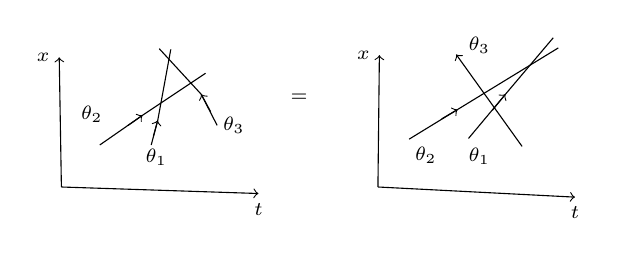
\begin{tikzpicture}[x=.92cm,y=.92cm,every node/.style={font=\scriptsize}]
\draw[->] (0,0) -- (2.72,-.09) node[below] {\(t\)};
\draw[->] (0,0) -- (-.03,1.79) node[left] {\(x\)};
\draw (.53,.58) -- (1.12,.99) -- (1.99,1.57);
\draw[->] (.92,.85) -- (1.12,.99);
\draw (1.24,.58) -- (1.33,.92) -- (1.51,1.90);
\draw[->] (1.27,.70) -- (1.33,.92);
\draw (2.15,.85) -- (1.93,1.28) -- (1.35,1.91);
\draw[->] (2.06,1.04) -- (1.93,1.28);
\node at (.42,1) {\(\theta_2\)};
\node at (1.31,.41) {\(\theta_1\)};
\node at (2.38,.85) {\(\theta_3\)};
\node at (3.28,1.23) {\(=\)};
\begin{scope}[xshift=4.02cm]
\draw[->] (0,0) -- (2.72,-.14) node[below] {\(t\)};
\draw[->] (0,0) -- (.02,1.82) node[left] {\(x\)};
\draw (.43,.66) -- (1.10,1.07) -- (2.49,1.92);
\draw[->] (.88,.94) -- (1.10,1.07);
\draw (1.25,.67) -- (1.76,1.28) -- (2.42,2.06);
\draw[->] (1.58,1.06) -- (1.76,1.28);
\draw[->] (1.99,.56) -- (1.08,1.83);
\node at (.66,.44) {\(\theta_2\)};
\node at (1.40,.42) {\(\theta_1\)};
\node at (1.40,1.96) {\(\theta_3\)};
\end{scope}
\end{tikzpicture}}\endgroup\par
The arrowhead on the descending \(\theta_3\) line on the left is retraced. Its direction is provisionally drawn up and to the left.}
\end{GelfandAdjacentEvidence}
\begin{GelfandAdjacentEvidence}{GELFAND-P000816}{5}


\begin{align*}
&\bigl(A_i(\theta_1)A_j(\theta_2)\bigr)A_k(\theta_3)\\
&=S_{ii_1}^{jj_1}A_{j_1}(\theta_2)\bigl(A_{i_1}(\theta_1)A_k(\theta_3)\bigr)=\\
&=S_{ii_1}^{jj_1}(\theta_{12})S_{i_1i_2}^{kk_1}(\theta_{13})
   \bigl(A_{j_1}(\theta_2)A_{k_1}(\theta_3)\bigr)A_{i_2}(\theta_1)=\\
&=S_{ii_1}^{jj_1}(\theta_{12})S_{i_1i_2}^{kk_1}(\theta_{13})S_{j_1j_2}^{k_1k_2}(\theta_{23})\\
&\qquad A_{k_2}(\theta_3)A_{j_2}(\theta_2)A_i(\theta)
\end{align*}
\Unclear{GELFAND-P000816}{chain-first-aj}{The letter \(A\) in \(A_j(\theta_2)\) in the first product is retraced. The original stroke is illegible.}
\end{GelfandAdjacentEvidence}
\begin{GelfandAdjacentEvidence}{GELFAND-P000816}{6}


\Unclear{GELFAND-P000816}{chain-first-s}{There is no written argument for \(S_{ii_1}^{jj_1}\) in the first equality.}
\end{GelfandAdjacentEvidence}
\begin{GelfandAdjacentEvidence}{GELFAND-P000816}{7}


\Unclear{GELFAND-P000816}{chain-reworked-theta}{The \(\theta\) in \(\theta_3\) after \(A_{k_2}\) in the final product is retraced. The original stroke is illegible.}
\end{GelfandAdjacentEvidence}
\begin{GelfandAdjacentEvidence}{GELFAND-P000816}{8}


\Unclear{GELFAND-P000816}{chain-last-factor}{The last factor is written \(A_i(\theta)\) without further numerical indices.}
\end{GelfandAdjacentEvidence}



\Needspace{7\baselineskip}
\begin{GelfandAdjacentEvidence}{GELFAND-P000817}{1}
\SourcePage{GELFAND-P000817}{67}
\uline{The eqs. take the form}:
\begin{equation*}
\begin{aligned}
&S^{kk_1}_{ii_1}(\theta)S^{jj_1}_{i_1i_2}(\theta+\theta')
  S^{j_1j_2}_{k_1k_2}(\theta')\\
&=S^{jj_1}_{kk_1}(\theta')S^{j_1j_2}_{ii_1}(\theta+\theta')
  S^{k_1k_2}_{i_1i_2}
\end{aligned}\tag{2}
\end{equation*}
\Unclear{GELFAND-P000817}{eq2-index-arguments}{The indices in (2) follow the manuscript. The last \(S\) has no written argument.}
\end{GelfandAdjacentEvidence}
\begin{GelfandAdjacentEvidence}{GELFAND-P000817}{2}


Over \(i_1,j_1,k_1\) sum.

In all: \(M^6\) eqs. for \(M^4\) fns. \(S^{\alpha\beta}_{ik}(\theta)\)

\(S\) plays the role of an \(S\)-matrix.

Put
\begin{equation*}
T_{\vec{\alpha},\vec{\beta}}(\theta)=
S^{\alpha_1\beta_1}_{i_1i_2}(\theta)
S^{\alpha_2\beta_2}_{i_2i_3}(\theta)
\cdot\;\cdot\;\cdot\;\cdot
S^{\alpha_N\beta_N}_{i_Ni_1}(\theta)\tag{3}
\end{equation*}
\Unclear{GELFAND-P000817}{eq3-middle-subscript}{The retraced lower indices of the middle factor provisionally read \(i_2i_3\).}
\end{GelfandAdjacentEvidence}
\begin{GelfandAdjacentEvidence}{GELFAND-P000817}{3}


\Unclear{GELFAND-P000817}{eq3-final-subscript}{The retraced lower indices of the last factor provisionally read \(i_Ni_1\), possibly \(i_Nk_1\).}
\end{GelfandAdjacentEvidence}
\begin{GelfandAdjacentEvidence}{GELFAND-P000817}{4}


The result will be a matrix \(M^N\times M^N\)
(“transfer matrix”)

[On the right:] \((\alpha_1,\ldots,\alpha_N)\) — indices.

\((\beta_1,\ldots,\beta_N)\) — 2nd set of inds.

It is asserted that
\begin{equation*}
[T(\theta),T(\theta')]=0\tag{4}
\end{equation*}
[To the right of zero, crossed out: \(\ldots\)]
\Incomplete{GELFAND-P000817}{eq4-crossed-right}{the entry is illegible}
\end{GelfandAdjacentEvidence}
\begin{GelfandAdjacentEvidence}{GELFAND-P000817}{5}


(by virtue of the factorization eqs.).

[On the left, an underlined entry is crossed out: \(\ldots\)]
\Incomplete{GELFAND-P000817}{eq4-crossed-left}{the entry is illegible}
\end{GelfandAdjacentEvidence}
\begin{GelfandAdjacentEvidence}{GELFAND-P000817}{6}


Factoriz. of the \(S\)-matr. is a consequence of a fin. number of conserv. laws.

\uline{Explicit form of the eqs. for \(M=2\)}

(case of Maxwell’s eqs.)
\begin{equation*}
\begin{cases}
A_1A_1=a\,A_1A_1+d\,A_2A_2\\
A_1A_2=b\,A_2A_1+c\,A_1A_2
\end{cases}
\qquad
\begin{pmatrix}
A_1(\theta_1),\ A_2(\theta_2)\\
a(\theta_1-\theta_2)
\end{pmatrix}\tag{5}
\end{equation*}
[On the right:] and 2 more eqs. with 1 replaced by 2
(with the same coeffs.)
(see \((5)_2\))

There are 4 fns. \(a,b,c,d\).

There could be 16 fns. In fact 5 or 6 fns. (from the eqs.).

Here 4 are retained

\uwave{The factorization eqs. give}:
\begin{equation*}
\left\{
\begin{aligned}
a(\theta)a(\theta+\theta')d(\theta')
&=d(\theta+\theta')a(\theta')\\
&\quad +b(\theta)b(\theta+\theta')d(\theta')
\end{aligned}
\right.\tag{6}
\end{equation*}
\SourceFigure{GELFAND-P000817}{eq6-dashed-row}{%
\par\begingroup\color{black}\GelfandFitDiagram{\begin{tikzpicture}[x=.004cm,y=.004cm]
\foreach \pos/\height/\len in {71/27/14,193/24/32,321/21/18,421/22/22,550/23/26,705/22/27,836/14/38,973/6/35,1075/2/28,1173/1/37,1289/3/41,1430/2/65,1556/4/40}
  \draw (\pos,\height) -- ++(\len,0);
\end{tikzpicture}}\endgroup\par
A row of short strokes beneath the written line of (6).}
\end{GelfandAdjacentEvidence}
\begin{GelfandAdjacentEvidence}{GELFAND-P000817}{7}


Here we have set \(c(\theta)\equiv1\) (the eqs. are homogeneous — let us divide).
\Unclear{GELFAND-P000817}{eq6-verb}{The verb provisionally reads «положено» (has been set), possibly «положим» (let us set).}
\end{GelfandAdjacentEvidence}
\begin{GelfandAdjacentEvidence}{GELFAND-P000817}{8}


[On the right:] (6 funct. eqs. in all)

\begin{equation*}
\begin{cases}
A_2A_2=a\,A_2A_2+d\,A_1A_1\\
A_2A_1=b\,A_1A_2+c\,A_2A_1
\end{cases}\tag*{\((5)_2\)}
\end{equation*}
\Unclear{GELFAND-P000817}{eq5-repeat-label}{The original mark under the retraced numeral 5 in \((5)_2\) is illegible.}
\end{GelfandAdjacentEvidence}
\begin{GelfandAdjacentEvidence}{GELFAND-P000817}{9}


\begin{equation*}
S^{\alpha\beta}_{ik}(0)=\delta_{i\beta}\delta_{\alpha k}\tag{7}
\end{equation*}
— \uline{init. condition}

\uwave{We obtain diff. eqs. from (6)}:
\begin{equation*}
\left\{
\begin{aligned}
\dot a&=\alpha a-\beta b+\gamma ad\\
\dot d&=\alpha d+\gamma(a^2-b^2)\\
a\dot b-b\dot a&=\beta(1-d^2)\\
d\dot b-b\dot d&=\alpha bd+\gamma b-\beta ad\\
&\text{and 2 more eqs.}
\end{aligned}
\right.
\qquad
\begin{aligned}
\dot a(0)&=\alpha\\
\dot b(0)&=\beta\\
\dot d(0)&=\gamma
\end{aligned}\tag{8}
\end{equation*}
\Unclear{GELFAND-P000817}{eq8-overwrite}{The \(b\dot a\) in the third line of (8) is retraced. The original strokes are illegible.}
\end{GelfandAdjacentEvidence}



\Needspace{7\baselineskip}
\begin{GelfandAdjacentEvidence}{GELFAND-P000818}{1}
\SourcePage{GELFAND-P000818}{unlabelled}
All the eqs. are independent.

3 algebr. relations arise, but one follows from the other 2.

Elliptic fns. are obtained (Baxter)

A noncommut., nonassoc. algebra arises, of quadruples of fns.
\Unclear{GELFAND-P000818}{top-quadruples}{The word reads «четверок» (quadruples). Strokes above «е» may indicate «ё».}
\end{GelfandAdjacentEvidence}
\begin{GelfandAdjacentEvidence}{GELFAND-P000818}{2}


It would be interesting to find an explicit \uline{realiz.} (e.g., on matrices)

\uwave{Yu. I. Manin’s idea}: take \uline{points} \uline{on} an ell. curve, of finite order

Let us expand
\begin{equation*}
T(\theta)=\sum_{\ell=0}^{\infty}I_{\ell}\theta^{\ell}\tag{9}
\end{equation*}
Then
\begin{equation*}
[I_n,I_m]=0\tag{10}
\end{equation*}
and in the example (\(M=2\)):
\begin{equation*}
\text{\uwave{\mbox{\(\displaystyle I_0^{-1}\,\text{\sout{(0)}}\,I_1\)}}}\,
\text{\sout{(0)}}
=\sum_{n=1}^{N}\sum_{\alpha=1}^{3}J_\alpha\sigma_n^\alpha\sigma_{n+1}^\alpha
\quad(=T^{-1}(0)\dot T(0))=H\tag{11}
\end{equation*}
\Unclear{GELFAND-P000818}{eq11-crossing-01}{A mark after \(I_0^{-1}\) is crossed out. It may read \((0)\).}
\end{GelfandAdjacentEvidence}
\begin{GelfandAdjacentEvidence}{GELFAND-P000818}{3}


\Unclear{GELFAND-P000818}{eq11-crossing-02}{A separate mark after \(I_1\) is crossed out. It too may read \((0)\).}
\end{GelfandAdjacentEvidence}
\begin{GelfandAdjacentEvidence}{GELFAND-P000818}{4}


Here
\[
\sigma_n^\alpha=1\otimes\ldots\otimes\sigma^\alpha\otimes\ldots\otimes1,
\qquad\sigma^\alpha\text{ — the Pauli matrices.}
\]
\begin{equation*}
[I_\ell,H]=0,\quad\ell=0,1,2,\ldots\tag{12}
\end{equation*}
The transfer matr. is written in terms of \(S\), i.e., in terms of ellipt. fns.

\(I_2\) contains 3 spins, and so on.

\uline{I. M. G.}\quad \(a,b,c,d\) — probably, \(SL(2,R)\)
\Unclear{GELFAND-P000818}{middle-maybe}{The word provisionally reads «наверное», possibly «наверно» (probably).}
\end{GelfandAdjacentEvidence}
\begin{GelfandAdjacentEvidence}{GELFAND-P000818}{5}


\(d=0\Rightarrow\) we obtain ordinary trig. fns. instead of ellipt. fns.

\SourceFigure{GELFAND-P000818}{middle-emphasis-strokes}{%
\par\begingroup\color{black}\GelfandFitDiagram{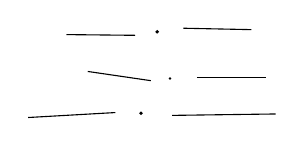
\begin{tikzpicture}[x=.9cm,y=.9cm]
\draw (.58,1.20)--(1.55,1.19);
\fill (1.86,1.24) circle[radius=.025cm];
\draw (2.23,1.29)--(3.19,1.27);
\draw (.88,.68)--(1.77,.55);
\fill (2.04,.58) circle[radius=.018cm];
\draw (2.42,.59)--(3.39,.59);
\draw (.04,.03)--(1.27,.10);
\fill (1.63,.09) circle[radius=.024cm];
\draw (2.07,.06)--(3.53,.08);
\end{tikzpicture}}\endgroup\par
Three rows of separate strokes beneath the entries about spins, \(SL(2,R)\), and trig. fns.}
\end{GelfandAdjacentEvidence}
\begin{GelfandAdjacentEvidence}{GELFAND-P000818}{6}


\uwave{General assertion} (now \(M\) is arbitrary):

Put
\begin{equation*}
\overset{\text{\sout{\(\ldots\)}}}{H}=
\sum_{n=1}^{N}\dot{S}_{ik}^{\alpha\beta}(0)\sigma_n^{i\beta}\sigma_{n+1}^{\alpha k}
=I_0^{-1}I_1
\qquad\text{(see (9)).}\tag{13}
\end{equation*}
\Incomplete{GELFAND-P000818}{eq13-crossing-over-h}{A mark above \(H\) is crossed out. The original sign is illegible.}
\end{GelfandAdjacentEvidence}
\begin{GelfandAdjacentEvidence}{GELFAND-P000818}{7}


\(\sigma\) — a matrix of size \(M\times M\).
\SourceFigure{GELFAND-P000818}{matrix-unit-schematic}{%
\par\begingroup\color{black}\GelfandFitDiagram{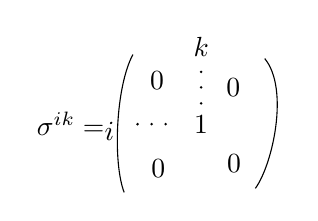
\begin{tikzpicture}[x=.85cm,y=.85cm]
\node at (-1.85,0) {\(\sigma^{ik}=\)};
\draw (-.92,1.04) .. controls (-1.18,.55) and (-1.22,-.58) .. (-1.05,-1.02);
\draw (1.05,.98) .. controls (1.42,.53) and (1.17,-.60) .. (.91,-.96);
\node at (-.56,.65) {\(0\)};
\node at (.58,.55) {\(0\)};
\node at (-.54,-.67) {\(0\)};
\node at (.59,-.59) {\(0\)};
\node at (.10,0) {\(1\)};
\foreach \x in {-.85,-.64,-.43} \fill (\x,0) circle[radius=.018cm];
\foreach \y in {.31,.55,.78} \fill (.10,\y) circle[radius=.018cm];
\node at (-1.27,-.11) {\(i\)};
\node at (.10,1.16) {\(k\)};
\end{tikzpicture}}\endgroup\par
basis in the space of matrices (\(1\) in position \(i,k\)).}
\end{GelfandAdjacentEvidence}
\begin{GelfandAdjacentEvidence}{GELFAND-P000818}{8}

\[
\sigma_n^{ik}=1\otimes\ldots\otimes\underset{n}{\sigma^{ik}}\otimes\ldots\otimes1
\]
We have a loc. Hamiltonian.

\Unclear{GELFAND-P000818}{hamiltonian-abbrev}{The abbreviation before “Hamiltonian” provisionally reads «лок.» (loc.).}
\end{GelfandAdjacentEvidence}
\begin{GelfandAdjacentEvidence}{GELFAND-P000818}{9}


Zamolodchikov obtained \uwave{particular} solutions (for different \(M\))

Let us use them for \(\underline{M=3}\), We obtain
\begin{equation*}
H=\sum_n\text{\sout{\(\ldots\)}}(\vec{S}_n\,\vec{S}_{n+1})^2-2\vec{S}_n\,\vec{S}_{n+1}\tag{14}
\end{equation*}
\Incomplete{GELFAND-P000818}{eq14-crossing}{An entry between the summation sign and the opening parenthesis is crossed out. The original signs are illegible.}
\end{GelfandAdjacentEvidence}


\(\underline{M=2}\) — isotr. Heisenberg ferromagnet
\begin{equation*}
H=\sum_n\vec{\sigma}_n\,\vec{\sigma}_{n+1}\tag{15}
\end{equation*}
spin \(1/2\) — there is nothing else inv.


\Needspace{7\baselineskip}
\begin{GelfandAdjacentEvidence}{GELFAND-P000819}{1}
\SourcePage{GELFAND-P000819}{68}
In (14): \(S^\alpha\) are such that
\begin{equation*}
[S^\alpha,S^\beta]=\varepsilon_{\alpha\beta\gamma}S^\gamma,\tag{16}
\end{equation*}
\(S^\alpha\) — inf. small rotation.
\Unclear{GELFAND-P000819}{upper-rotation-abbreviation}{The first abbreviation before “small rotation” provisionally reads «беск.» (inf.). Some strokes overlap.}
\end{GelfandAdjacentEvidence}
\begin{GelfandAdjacentEvidence}{GELFAND-P000819}{2}


(rep. of the group \(SO(3)\))

adj. \(=\) standard

There are no parameters here

\(\underline{\underline{M=3}}\Rightarrow\) there is no general soln.

(!) \uwave{It is unknown how to add parameters to Ham. (14) so as to fit Zamolodchikov’s scheme.}

This scheme cont. all fully integr. quant. systems (2-dimensional)

(\(\Rightarrow\) classical ones too after taking the quasiclass. limit).

\begin{equation*}
H=\sum_{n=1}^{N}\dot S_{ik}^{\alpha\beta}(0)
 \sigma_n^{i\beta}\sigma_{n+1}^{\alpha k};\tag{17}
\end{equation*}
\uwave{I.M.G.’s question}: rels. on \(S\) — of Maurer–Cartan type

(17) — the most general form of Ham. with nearest-neighbor interact.

It \uline{always} has a nontriv. integral, since the diff. eqs. extend to the 2nd neighborhood.
\[
S=S(0)+S'(0)\theta+\frac{S''(0)\theta^2}{2}
\]
\(S''\) is recovered.

\(A_i(\theta)\) are matrices \(\Rightarrow\) there is \uwave{assoc.} automatically

There is a way to multiply algebras.

Suppose we found \(S_{ik}^{\alpha\beta}\). Let us construct

(e.g. \(\underline{M=2}\))
\begin{equation*}
 L^{ik}_{\vec\alpha\vec\beta}
 =S_{ij_1}^{\alpha_1\beta_1}S_{j_2j_3}^{\alpha_2\beta_2}.\, .
 S_{j_Nk}^{\alpha_N\beta_N}
 \qquad\text{(we did not take the trace)}\tag{18}
\end{equation*}
\Unclear{GELFAND-P000819}{eq18-l-indices}{The lower indices of \(L\) are set as \(\vec\alpha\vec\beta\). There is a crossed-out entry alongside them.}
\end{GelfandAdjacentEvidence}
\begin{GelfandAdjacentEvidence}{GELFAND-P000819}{3}


\Unclear{GELFAND-P000819}{eq18-product-indices}{The second factor has lower indices \(j_2j_3\), while the first ends with \(j_1\). Two dots separate the second and last factors.}
\end{GelfandAdjacentEvidence}
\begin{GelfandAdjacentEvidence}{GELFAND-P000819}{4}


We get the matrix
\begin{equation*}
L=\begin{pmatrix}L_{11}&L_{12}\\L_{21}&L_{22}\end{pmatrix}
=(L^{\alpha\beta})\tag{19}
\end{equation*}
its elems. — \uline{are matrices too}.

[crossed out: \sout{\(\ldots\)}]
Rels. of type (2) \(-\ -\) hold for the matrix \(L\)
\Incomplete{GELFAND-P000819}{lower-left-deletion}{The crossed-out sign before “Rels.” is illegible.}
\end{GelfandAdjacentEvidence}
\begin{GelfandAdjacentEvidence}{GELFAND-P000819}{5}


\begin{equation*}
S_{ik}^{\alpha\mu}S_{kj}^{\beta\nu}S_{\mu\gamma}^{\nu\delta}
=S_{\beta\nu}^{\alpha\mu}S_{ik}^{\mu\gamma}S_{kj}^{\nu\delta}
\tag*{(2)\('\)}
\end{equation*}
\(L^{ik}\) — matr. \(M^N\times M^N\) for all \(i,k\).

There are relations:
\begin{equation*}
\begin{array}{rccccccc}
 &L^{\alpha\mu}&L^{\beta\nu}&S_{\mu\gamma}^{\nu\delta}
 &=&S_{\beta\nu}^{\alpha\mu}&L^{\mu\gamma}&L^{\nu\delta}.\\
 \text{arguments:}&\theta&\theta'&\theta-\theta'
 &&\theta-\theta'&\theta'&\theta
\end{array}\tag{20}
\end{equation*}
\Unclear{GELFAND-P000819}{eq20-argument-layout}{The arguments are written under their corresponding factors. On the right, the two \(L\) factors are marked first \(\theta'\), then \(\theta\).}
\end{GelfandAdjacentEvidence}



\Needspace{7\baselineskip}
\begin{GelfandAdjacentEvidence}{GELFAND-P000820}{1}
\SourcePage{GELFAND-P000820}{unlabelled}
Now suppose
\begin{equation*}
A_{\alpha\mu}=L^{\alpha\mu}\tag{21}
\end{equation*}
We get a new algebra of higher order

\SourceFigure{GELFAND-P000820}{toroidal-grid}{%
\begingroup\color{black}\GelfandFitDiagram{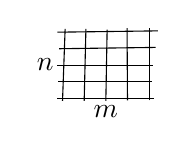
\begin{tikzpicture}[x=.55cm,y=.42cm]
\draw (-.12,0)--(2.12,0);
\draw (-.10,.5)--(2.06,.5);
\draw (-.12,1)--(2.10,1);
\draw (-.08,1.5)--(2.15,1.54);
\draw (-.12,2)--(2.20,2.04);
\draw (0,-.08)--(.06,2.1);
\draw (.5,-.08)--(.54,2.1);
\draw (1,-.08)--(1.03,2.08);
\draw (1.5,-.06)--(1.49,2.12);
\draw (2,-.06)--(2,2.12);
\node at (-.40,1.02) {\(n\)};
\node at (1,-.40) {\(m\)};
\end{tikzpicture}}\endgroup\par
2-dim. lattice rolled into a torus.}
\end{GelfandAdjacentEvidence}
\begin{GelfandAdjacentEvidence}{GELFAND-P000820}{2}


Onsager in ’44 — 2-dim. Ising model

\mbox{—\textbar\textbar—} ’65 — devis. commut. transfer matrix.
\Unclear{GELFAND-P000820}{onsager-verb}{The abbreviation before “commut.” provisionally reads «прид.» (devis.). «пред.» (propos.) is also possible.}
\end{GelfandAdjacentEvidence}
\begin{GelfandAdjacentEvidence}{GELFAND-P000820}{3}


\[
\sigma_{n,m}=\pm1
\]
We need to calc. the sum:
\begin{equation*}
Z=\sum_{\{\sigma_{n,m}\}}
e^{J_1\sum\sigma_{n,m}\sigma_{n,m+1}+J_2\sum\sigma_{n,m}\sigma_{n+1,m}\text{ \sout{…}}}
\tag{22}
\end{equation*}
\Incomplete{GELFAND-P000820}{exponent-cancellation}{The entry at the end of the exponent is crossed out. Its signs are illegible.}
\end{GelfandAdjacentEvidence}
\begin{GelfandAdjacentEvidence}{GELFAND-P000820}{4}


(nearest-neighbor interact.)

Idea:
\begin{equation*}
Z=\operatorname{Tr}T^N\tag{23}
\end{equation*}

\SourceFigure{GELFAND-P000820}{diagonal-dots}{%
\begingroup\color{black}\GelfandFitDiagram{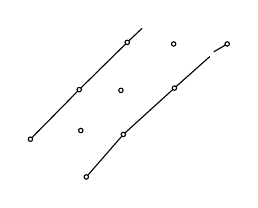
\begin{tikzpicture}[x=.010cm,y=.010cm]
\draw (27,59)--(89,122)--(150,182)--(169,200);
\draw (98,11)--(145,65)--(210,124)--(255,164);
\draw (260,170)--(277,180);
\foreach \x/\y in {27/59,89/122,150/182,91/70,142/121,209/180,98/11,145/65,210/124,277/180}
  \draw[fill=white] (\x,\y) circle[radius=.028cm];
\end{tikzpicture}}\endgroup\par
The strokes meet at the top circle on the left line. A separate arrowhead cannot be distinguished.}
\end{GelfandAdjacentEvidence}
\begin{GelfandAdjacentEvidence}{GELFAND-P000820}{5}


[At right:] \uwave{Onsager}: we go along the diagonals (we sum over the spins on the interm. diag.)
\begin{equation*}
T_{\vec\alpha\,\vec\beta}=S_1\ldots S_n,\tag{24}
\end{equation*}
where

\SourceFigure{GELFAND-P000820}{eq25-diamond}{%
\begingroup\color{black}\GelfandFitDiagram{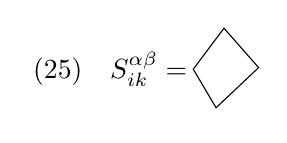
\begin{tikzpicture}[baseline=-.5ex]
\node[anchor=east,inner sep=2pt] at (0,.5) {\((25)\quad S_{ik}^{\alpha\beta}=\)};
\draw (0,.5)--(.39,1.02)--(.83,.52)--(.29,.01)--cycle;
\end{tikzpicture}}\endgroup}
\end{GelfandAdjacentEvidence}
\begin{GelfandAdjacentEvidence}{GELFAND-P000820}{6}


We get the tr. matr. \qquad \(T(J_1,J_2)\)

\uline{Prop.}

\(T(J_1,J_2)\) commut. wh
\Incomplete{GELFAND-P000820}{bottom-fragment}{The last visible letters are «пр», possibly the start of «при» (“when”). The entry breaks off.}
\end{GelfandAdjacentEvidence}



\clearpage
\pdfbookmark[0]{Chapter 15}{gelfand-archive-chapter-15}
\section*{Chapter 15}
\Needspace{7\baselineskip}
\begin{GelfandAdjacentEvidence}{GELFAND-P000821}{1}
\SourcePage{GELFAND-P000821}{unlabelled}
[At the upper left, crossed out: \sout{22…}]
\Unclear{GELFAND-P000821}{cancelled-page-label}{The start of the crossed-out entry provisionally reads “22”. The ending is illegible.}
\end{GelfandAdjacentEvidence}
\begin{GelfandAdjacentEvidence}{GELFAND-P000821}{2}


\uuline{26.2.79} \qquad \uline{Gelfand Sem.}

\uuline{S. Gelfand} \quad \uline{from Manin’s lecture}

This concerns the relation of Y.–M. solns to alg.-geom. objects

(solns need not be self-dual)

— Witten; indep. Yasskin, Isenberg, Green (1978)
\Unclear{GELFAND-P000821}{researcher-names}{The names are written «Яскин, Айзенберг, Грин».}
\end{GelfandAdjacentEvidence}
\begin{GelfandAdjacentEvidence}{GELFAND-P000821}{3}


\[
\widehat{\mathbb{C}M}=G(4,2)\qquad
\text{(Grassmannian set of 2-dim. compl. planes in \(\mathbb{C}^4\))}
\]
\Incomplete{GELFAND-P000821}{grassmannian-cancelled-index}{There is a heavily inked-out entry at the lower right of \(G\). Its sign is illegible.}
\end{GelfandAdjacentEvidence}
\begin{GelfandAdjacentEvidence}{GELFAND-P000821}{4}


[Below \(G(4,2)\):] (compl. Grassmannian set)

[Below the formula at left, a vertical line to the label:] complexif. Minkowski space

(and compactif.)

(in \(G(4,2)\) there is an open subset isom. to \(\mathbb{C}^4\)).

\uwave{S. Gelfand}

\(M^4\) (Mink. space) with conf. metric is compactif. i.e. light cone

(at infinity). All conf. transf. are also \(SU(2,2)\)

We get the stat. group \(SO(3,1)\)

\begin{equation*}
\widehat{M^4}=SU(2,2)/SO(3,1)\tag{1}
\end{equation*}
\Unclear{GELFAND-P000821}{minkowski-quotient}{The denominator in the manuscript is \(SO(3,1)\).}
\end{GelfandAdjacentEvidence}
\begin{GelfandAdjacentEvidence}{GELFAND-P000821}{5}


Now complexify \(SU(2,2)\) and \(SO(3,1)\) and take the quotient

\begin{equation*}
(SU(2,2)=SO(4,2))\tag{2}
\end{equation*}

\(SU(2,2)\) — conf. group for \(M^4\)

\uwave{Geometric picture.}

In \(\mathbb{C}P^3\) consid. [crossed out: \sout{cone}]
[inserted above: surface] (real 5-dimensional)
\Unclear{GELFAND-P000821}{surface-cancellation}{The crossed-out word provisionally reads “cone”. “Surface” is written above it.}
\end{GelfandAdjacentEvidence}
\begin{GelfandAdjacentEvidence}{GELFAND-P000821}{6}


\begin{equation*}
R=\{z:|z_1|^2+|z_2|^2-|z_3|^2-|z_4|^2=0\}\subset\mathbb{C}P^3
\tag{3}
\end{equation*}

\SourceFigure{GELFAND-P000821}{projectivization-arrow}{%
\begingroup\color{black}\GelfandFitDiagram{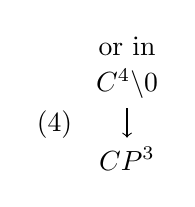
\begin{tikzpicture}[baseline=(current bounding box.center)]
\node at (0,1.28) {or in};
\node (total) at (0,.80) {\(\mathbb{C}^4\backslash0\)};
\node (base) at (0,-.15) {\(\mathbb{C}P^3\)};
\node at (-.92,.29) {(4)};
\draw[->] (total)--(base);
\end{tikzpicture}}\endgroup\par
acts \(GL(4,\mathbb{C})\); surf. (3) is preserved by the group \(SU(2,2)\)}
\end{GelfandAdjacentEvidence}
\begin{GelfandAdjacentEvidence}{GELFAND-P000821}{7}


\(G(4,2)\) — set of lines in \(\mathbb{C}P^3\);

(or 2-dim. subspaces in \(\mathbb{C}^4\))

On surf. (3) there lies wholly a \uwave{set of lines} of real dimension 4.

\(SU(2,2)\) carries over to this set.

\uline{Theorem 1.} \uwave{Contain. set of these lines — Minkowski space.}
\Unclear{GELFAND-P000821}{theorem-opening-word}{The first abbreviation provisionally reads «Содерж.» (“contain.”), possibly «Соотв.» (“correspond.”).}
\end{GelfandAdjacentEvidence}
\begin{GelfandAdjacentEvidence}{GELFAND-P000821}{8}


[crossed out: \sout{\uline{Proof}}]
\Unclear{GELFAND-P000821}{cancelled-proof-heading}{The cancelled heading provisionally reads «Доказ.» (“Proof”).}
\end{GelfandAdjacentEvidence}


The lines on surf. (3) are parametriz. by unit. matrices of order 2
\[
(z_3,z_4)=U(z_1,z_2),\qquad U\in U(2)
\]

\uwave{Minkowski metric.}

Consid. a fixed line \(L_0\) on \(R\). Consid. all other lines on \(R\), that intersect it.
\uwave{We get a 3-dim. cone} \(K_{L_0}\). It is preserved under all transf. preserving \(L_0\).
We get \(SO(3,1)\) and a cone called the \uwave{light cone}.

The points of surf. \(R\) can be interpreted as rays of light.

One can collect \uwave{all points of intersection of} \(L\subset R\) with \(L_0\).
This gives a generator of the cone (light cone).


\Needspace{7\baselineskip}
\begin{GelfandAdjacentEvidence}{GELFAND-P000822}{1}
\SourcePage{GELFAND-P000822}{2}
Cf.: the quaternionic version (it was discussed at some point).

Stat. subgroup:
\[
GL(2,\mathbb{C})\times\mathbb{R}^3\qquad(?)
\]

The conf. group is obtained by adding inversion \(\frac{1}{\tau}\) (\(\tau\) — Minkowski dist.)
to the motions (the grp. of \uline{Poincaré}).

\[
\begin{array}{@{}l@{}}
X=G(4,2)\\[-.3ex]
\cup\\[-.3ex]
\mathbb{C}^4\ni(z_1,z_2,z_3,z_4)
\end{array}
\]
\Unclear{GELFAND-P000822}{containment-mark}{The sign below \(X\) resembles \(\cup\). It is set in the same vertical position.}
\end{GelfandAdjacentEvidence}
\begin{GelfandAdjacentEvidence}{GELFAND-P000822}{2}


There we consid. holom. connections satisfying the Y.–M. eqs.

\(G\) — a compl. Lie grp.; \(\mathfrak g\) — its Lie algebra.

\((A_1(z),A_2(z),A_3(z),A_4(z))\) — holom. fns. with values in \(\mathfrak g\)

(holom. in an open region)

\begin{equation*}
F_{\mu\nu}(z)=\partial_\mu A_\nu-\partial_\nu A_\mu+[A_\mu,A_\nu],
\qquad \partial_\mu=\frac{\partial}{\partial z_\mu}.
\tag{5}
\end{equation*}

Connection form:
\[
\omega=\sum A_\mu(z)\,dz_\mu
\]

\(F\) — the curvature form of this connection (again with values in the Lie alg.)

\uwave{Y.–M. eqs.}
\begin{equation*}
\sum_{\mu=1}^{4}\left\{\frac{\partial F_{\mu\nu}}{\partial z_\mu}
 +[F_{\mu\nu},A_\mu]\right\}=0,\qquad \nu=1,2,3,4.
\tag{6}
\end{equation*}
\Unclear{GELFAND-P000822}{yang-mills-commutator-order}{In (6) the manuscript has \([F_{\mu\nu},A_\mu]\) after the plus sign.}
\end{GelfandAdjacentEvidence}
\begin{GelfandAdjacentEvidence}{GELFAND-P000822}{3}


\uwave{I.M.G.} \quad Landau: “the Lagrangian is a corpse” thought that one need only know the \(S\)-matrix, and that is all.

The corresp. real eqs. are obtained from the Lagrangian:

\begin{equation*}
L=\operatorname{tr}\int F_{\mu\nu}F^{\mu\nu}\,d^4x
\tag{7}
\end{equation*}

Solutions of (6) are related to certain objects of compl. analytic geometry.

From \(\mathbb{C}^4\) we construct
\[
\underset{\text{lines in \(\mathbb{C}^4\)}}{\mathbb{C}P^3}
\qquad\text{and}\qquad
\underset{\text{hyperpl. in \(\mathbb{C}^4\)}}{\mathbb{C}P^3}
\]

[Crossed out before the formula: \sout{…}]
\Incomplete{GELFAND-P000822}{quadric-cancelled-sign}{A separate sign is heavily crossed out. Its numeral cannot be established.}
\end{GelfandAdjacentEvidence}
\begin{GelfandAdjacentEvidence}{GELFAND-P000822}{4}


\begin{equation*}
\mathbb{C}P^3\times\mathbb{C}P^3\supset
 Q=\{(\ell,\pi)\mid\ell\subset\pi\},\qquad \dim_{\mathbb{C}}G=5
\tag{8}
\end{equation*}
\Unclear{GELFAND-P000822}{dimension-glyph}{The letter after \(\dim_{\mathbb{C}}\) provisionally reads \(G\), possibly \(Q\). The first \(Q\) on the same line has a closed upper loop.}
\end{GelfandAdjacentEvidence}
\begin{GelfandAdjacentEvidence}{GELFAND-P000822}{5}


[Vertical stroke down from \(Q\):] the set defin. duality (partial fl-ags)
\Unclear{GELFAND-P000822}{quadric-caption-word}{The abbreviation before “duality” is provisionally set as «зад.» (“defin.”). The initial descender and final loop admit another reading.}
\end{GelfandAdjacentEvidence}
\begin{GelfandAdjacentEvidence}{GELFAND-P000822}{6}


\uwave{2nd object}.

(9) \uwave{Holomorphic bundles on} \(Q\) \uwave{with structure group} \(G\), \uwave{which}
\uwave{extend holom. to the 3rd infinitesim. neighborhood of} \(Q\) in \(\mathbb{C}P^3\times\mathbb{C}P^3\).

(In fact everything is over subsets).
\Unclear{GELFAND-P000822}{subset-word-overwriting}{Several letters in “subsets” are overwritten. The earlier form is illegible.}
\end{GelfandAdjacentEvidence}


All connections \(\Longleftrightarrow\) all bundles (not necessarily extending to the 3rd infinit. neighborhood)


\Needspace{7\baselineskip}
\begin{GelfandAdjacentEvidence}{GELFAND-P000823}{1}
\SourcePage{GELFAND-P000823}{unlabelled}
\uline{A. Beilinson}

on \(G(4,2)\) we consid. the full flag space \(F\) (line, plane, hyperpl.)

\SourceFigure{GELFAND-P000823}{left-margin-sketches}{%
\begingroup\color{black}\GelfandFitDiagram{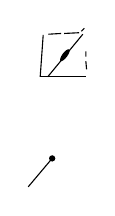
\begin{tikzpicture}[x=.95cm,y=.95cm]
\draw (-.14,.15)--(-.10,.71);
\draw (-.14,.15)--(.47,.15);
\draw (-.03,.72)--(.14,.73) (.18,.73)--(.38,.74) (.41,.76)--(.45,.80);
\draw (.48,.25)--(.47,.36) (.47,.42)--(.47,.49);
\draw (-.04,.15)--(.43,.72);
\fill[rotate around={53:(.19,.44)}] (.19,.44) ellipse[x radius=.092cm,y radius=.032cm];
\draw (-.30,-1.32)--(.02,-.94);
\fill (.02,-.94) circle[radius=.04cm];
\end{tikzpicture}}\endgroup\par
The upper and right edges are broken. The slanted strokes have thickened parts.}
\end{GelfandAdjacentEvidence}
\begin{GelfandAdjacentEvidence}{GELFAND-P000823}{2}


\SourceFigure{GELFAND-P000823}{flag-projections}{%
\begingroup\color{black}\GelfandFitDiagram{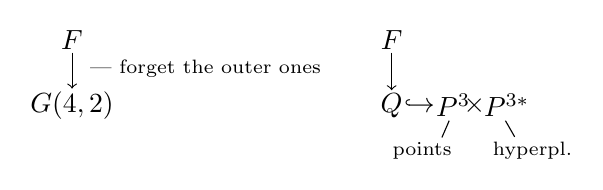
\begin{tikzpicture}[x=.84cm,y=.76cm,every node/.style={inner sep=1pt}]
\node (lf) at (0,0) {\(F\)};
\node (lg) at (0,-1.1) {\(G(4,2)\)};
\draw[->] (lf)--(lg);
\node[font=\scriptsize,anchor=west] at (.22,-.48) {— \uwave{forget the outer ones}};
\begin{scope}[xshift=1.48cm]
\node (rf) at (3.07,0) {\(F\)};
\node (rq) at (3.07,-1.1) {\(Q\)};
\draw[->] (rf)--(rq);
\node at (3.49,-1.1) {\(\hookrightarrow\)};
\node at (4,-1.1) {\(P^3\)};
\node at (4.32,-1.1) {\(\times\)};
\node at (4.81,-1.1) {\(P^{3*}\)};
\draw (3.94,-1.35)--(3.83,-1.63) (4.79,-1.35)--(4.93,-1.62);
\node[font=\scriptsize] at (3.53,-1.85) {points};
\node[font=\scriptsize] at (5.20,-1.85) {hyperpl.};
\end{scope}
\end{tikzpicture}}\endgroup\par
In the right diagram a hooked arrow points right from \(Q\).}
\end{GelfandAdjacentEvidence}
\begin{GelfandAdjacentEvidence}{GELFAND-P000823}{3}


[Crossed out to the right of the right-hand \(F\): \sout{…}]
\Incomplete{GELFAND-P000823}{cancelled-right-projection}{Strokes cover a vertical entry. The original sign is illegible.}
\end{GelfandAdjacentEvidence}
\begin{GelfandAdjacentEvidence}{GELFAND-P000823}{4}


\SourceFigure{GELFAND-P000823}{point-hyperplane-sketches}{%
\begingroup\color{black}\GelfandFitDiagram{\begin{tikzpicture}[x=1cm,y=1cm]
\draw (0,0)--(.14,.57) (.17,.59)--(.85,.72) (0,0)--(.86,.20);
\draw (.86,.25)--(.86,.38) (.87,.56)--(.87,.60);
\fill (.32,.42) circle[radius=.046cm];
\fill (1.74,.81) circle[radius=.039cm];
\draw (3.11,.45)--(3.17,.84) (3.19,.89)--(3.77,.93) (3.11,.45)--(3.77,.46);
\draw (3.74,.54)--(3.78,.69) (3.79,.75)--(3.82,.82);
\draw (3.90,.95)--(4.03,1.09);
\end{tikzpicture}}\endgroup\par
There is a separate point between the figures. A short upper-right stroke has an unclear relation to the outline.}
\end{GelfandAdjacentEvidence}
\begin{GelfandAdjacentEvidence}{GELFAND-P000823}{5}


\[
\begin{gathered}
(E,\nabla)\\
\text{bundle with connection}\\
\text{on }G(4,2)
\end{gathered}
\]

\uwave{The fiber of the right bundle is isom. to} \(\mathbb{C}P^1\)

Under the left projection it goes to \(\mathbb{C}P^1\)

on \(\mathbb{C}P^1\) the bundle trivializes (canonically), since the curvature \(=0\) on account of the dimension being one

(fund. group \(=0\)).

The connection (\(\omega\)) we lift to \(F\) and try to descend to \(Q\).
\Unclear{GELFAND-P000823}{connection-parenthesis}{The symbol in parentheses provisionally reads \(\omega\). Its shape differs from \(\nabla\) in the pair \((E,\nabla)\).}
\end{GelfandAdjacentEvidence}
\begin{GelfandAdjacentEvidence}{GELFAND-P000823}{6}


[Below the line] (from \(G(4,2)\))

It is on \(\forall\) fibers trivial \(\Rightarrow\) can be carried over to \(Q\)

We get \(\widetilde E\) — a holom. vect. bundle on \(Q\)
\Unclear{GELFAND-P000823}{bundle-accent}{The first \(E\) has a thick, almost horizontal stroke above it. The wavy mark is clearer lower down.}
\end{GelfandAdjacentEvidence}
\begin{GelfandAdjacentEvidence}{GELFAND-P000823}{7}


\SourceFigure{GELFAND-P000823}{lower-notation}{%
\((E,\nabla)\longleftrightarrow\widetilde E\)\par
\(\widetilde E\) is triv. on \(\mathbb{C}P^1\times\mathbb{C}P^1\)\par
\begingroup\color{black}\GelfandFitDiagram{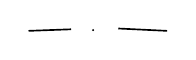
\begin{tikzpicture}
\draw[semithick] (0,0)--(.54,.02) (1.14,.03)--(1.76,0);
\fill (.82,.01) circle[radius=.014cm];
\end{tikzpicture}}\endgroup\par
Two strokes and a dot between them appear under the final line.}
\end{GelfandAdjacentEvidence}



\Needspace{7\baselineskip}
\begin{GelfandAdjacentEvidence}{GELFAND-P000824}{1}
\SourcePage{GELFAND-P000824}{unlabelled}
\uuline{5/III-79} \qquad \uline{Gelfand Sem.}

\uuline{D. B. Fuchs.}

\uuline{On \(\infty\)-dimensional Lie algebras}

(construction and classification).

\uwave{Graded Lie alg.}:
\[
\mathfrak g=\bigoplus_{i\in\mathbb{Z}}\mathfrak g_i,\qquad
[\mathfrak g_i,\mathfrak g_j]\subset\mathfrak g_{i+j}
\]
hence \(\mathfrak g_0\) — a subalg., and all the \(\mathfrak g_i\) —
\(\mathfrak g_0\)-modules.

\uwave{Cartan’s construction}:
\begin{equation*}
\mathfrak g_i=0\quad\text{for }i<i_0.\tag{1}
\end{equation*}
\uwave{Transitivity}: there is a homom.
\begin{equation*}
\mathfrak g_i\to\operatorname{Hom}(\mathfrak g_{-1},\mathfrak g_{i-1})\tag{2}
\end{equation*}
\begin{equation*}
\mathfrak g_i\to\operatorname{Hom}(\mathfrak g_1,\mathfrak g_{i+1})\tag{3}
\end{equation*}
\begin{equation*}
\left\{\begin{aligned}
i\ge0&\ \Rightarrow\ (2)\ \text{monomorphic}\\
i\le0&\ \Rightarrow\ (3)\ \text{monomorphic}
\end{aligned}\right.\tag{4}
\end{equation*}
Then there is Cartan’s classification thm.: there are 4 series.

1) \(W_n\) — polynomial vect. fields on \(\mathbb{C}^n\):
\begin{equation*}
\sum p_i(x_1,\ldots,x_n)\frac{\partial}{\partial x_i}\tag{5}
\end{equation*}
\(\deg\frac{\partial}{\partial x_i}=-1,\)
[crossed out: \sout{…}]
\(\deg x_i=1.\)
\Incomplete{GELFAND-P000824}{degree-cancel}{A sign between the two degrees is crossed out. Its original form is illegible.}
\end{GelfandAdjacentEvidence}
\begin{GelfandAdjacentEvidence}{GELFAND-P000824}{2}


Here

\(\mathfrak g_0\) — \uwave{matrix alg.}(!)
(gen. by the fields \(x_j\frac{\partial}{\partial x_i}\)).

2) divergence-free vect. fields \(S_n\)
\Unclear{GELFAND-P000824}{divergence-series-mark}{A short rising stroke joins the upper-right edge of \(S\). It may be the end of the letter or a prime mark.}
\end{GelfandAdjacentEvidence}


3) Hamiltonian \(H_n\)

4) contact \(K_n\) \qquad pres. the cont. struct. in \(\mathbb{C}^{2n+1}\)

(description of the grading is omitted)

(all are polynomial)

\uline{Idea of the proof}:

Cart. prolongation.

For simplicity assume \(i_0=-1\) (in (1))
\begin{equation*}
\mathfrak g=\mathfrak g_{-1}\oplus\mathfrak g_0\oplus\cdots\tag{6}
\end{equation*}
From \(\mathfrak g_0\) and \(\mathfrak g_{-1}\) everything is recovered


\Needspace{7\baselineskip}
\begin{GelfandAdjacentEvidence}{GELFAND-P000825}{1}
\SourcePage{GELFAND-P000825}{10}
We have:
\begin{equation*}
\mathfrak g_1\subset\operatorname{Hom}(\mathfrak g_{-1},\mathfrak g_0)\tag{7}
\end{equation*}
\[
\begin{gathered}
f\in\operatorname{Hom}(\mathfrak g_{-1},\mathfrak g_0),\quad
\alpha_1,\alpha_2\in\mathfrak g_{-1}\quad\Rightarrow\\
\Rightarrow
\end{gathered}
\]
\begin{equation*}
f(\alpha_1)\alpha_2=f(\alpha_2)\alpha_1\tag{8}
\end{equation*}
(from the Jacobi id.)
\Unclear{GELFAND-P000825}{eq8-retraced-index}{The subscript on the second \(\alpha\) on the left is retraced. Its visible form reads 2.}
\end{GelfandAdjacentEvidence}
\begin{GelfandAdjacentEvidence}{GELFAND-P000825}{2}


Let
\begin{equation*}
\mathfrak g_1=\{f\in\operatorname{Hom}(\mathfrak g_{-1},\mathfrak g_0)
\mid f(\alpha_1)\alpha_2=f(\alpha_2)\alpha_1\}\tag{9}
\end{equation*}
\begin{equation*}
\begin{aligned}
\mathfrak g_2 &\subset\operatorname{Hom}(\mathfrak g_{-1},\mathfrak g_1)
\subset\operatorname{Hom}(\mathfrak g_{-1},\operatorname{Hom}(\mathfrak g_{-1},\mathfrak g_0))=\\
&=\operatorname{Hom}(\mathfrak g_{-1}\otimes\mathfrak g_{-1},\mathfrak g_0)
\end{aligned}\tag{10}
\end{equation*}
Jacobi id. \(\Rightarrow\)
\begin{equation*}
f(\alpha_1\otimes\alpha_2)\alpha_3\text{ — symm. in all 3 vars.}\tag{11}
\end{equation*}
Put
\begin{equation*}
\mathfrak g_2=\left\{\begin{aligned}
&f\in\operatorname{Hom}(\mathfrak g_{-1}\otimes\mathfrak g_{-1},\mathfrak g_0)\mid\\
&f(\alpha_1\otimes\alpha_2)\alpha_3\text{ symm. in all vars.}
\end{aligned}\right\}\tag{12}
\end{equation*}
and then
\begin{equation*}
\mathfrak g_k=\left\{\begin{aligned}
&f\in\operatorname{Hom}(\overset{k}{\bigotimes}\mathfrak g_{-1},\mathfrak g_0)\mid\\
&f(\alpha_1\otimes\cdots\otimes\alpha_k)\alpha_{k+1}\text{ is symmetric}
\end{aligned}\right\}\tag{13}
\end{equation*}
The commutator in \(\bigl[\bigoplus \mathfrak g_k\bigr]\) — ?

with \(\mathfrak g_{-1}\) the commut. is already defined, with \(\mathfrak g_0\) — likewise.
\[
\alpha\in\mathfrak g_k,\quad \beta\in\mathfrak g_\ell\quad\Rightarrow\quad
\text{to def. }[\alpha,\beta]\text{ one needs to specify}
\]
\[
[[\alpha,\beta],\delta],\qquad\delta\in\mathfrak g_{-1}
\]
\Unclear{GELFAND-P000825}{bracket-letter}{The same letter in both places provisionally reads \(\delta\). \(\gamma\) is also possible.}
\end{GelfandAdjacentEvidence}
\begin{GelfandAdjacentEvidence}{GELFAND-P000825}{3}


Jacobi id. \(\rightsquigarrow\) into terms def. by induction.

[Crossed out: \sout{We need \(\mathfrak g_0\) and \(\mathfrak g_{-1}\) to be …}]
\Unclear{GELFAND-P000825}{cancel-prefix}{The start of the crossed-out line is provisional. Strokes cross the connector between the two \(\mathfrak g\) terms and the sign before the index 1.}
\end{GelfandAdjacentEvidence}
\begin{GelfandAdjacentEvidence}{GELFAND-P000825}{4}


\Incomplete{GELFAND-P000825}{cancel-ending}{The end of the crossed-out line is illegible.}
\end{GelfandAdjacentEvidence}


\(\mathfrak g_0,\mathfrak g_{-1}\) can be arbitrary. Simplicity is an addl. condition.

But as a rule we get a finite-dimensional algebra!!

\(\infty\)-dimensionality — \uline{luck}.

\uline{Another constr.}

Let \(\mathfrak g_{-1},\mathfrak g_0\) be given,\qquad
\(\mathfrak g_0\subset\operatorname{End}(\mathfrak g_{-1})\).


\Needspace{7\baselineskip}
\begin{GelfandAdjacentEvidence}{GELFAND-P000826}{1}
\SourcePage{GELFAND-P000829}{12}
\uline{2nd constr.} \quad Suppose

There is an involution in \(\mathfrak g\): \(\tau:\mathfrak g\to\mathfrak g\). Then

\SourceFigure{GELFAND-P000829}{eigenspace-callouts}{%
\begingroup\color{black}\GelfandFitDiagram{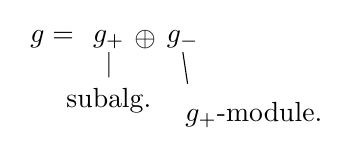
\begin{tikzpicture}[every node/.style={inner sep=1pt}]
\node at (0,0) {\(\mathfrak g=\)};
\node (plus) at (.72,0) {\(\mathfrak g_+\)};
\node at (1.18,0) {\(\oplus\)};
\node (minus) at (1.66,0) {\(\mathfrak g_-\)};
\node[anchor=north] at (.72,-.58) {subalg.};
\node[anchor=north west] at (1.65,-.75) {\(\mathfrak g_+\)-module.};
\draw (plus.south)--(.72,-.48) (minus.south)--(1.72,-.56);
\end{tikzpicture}}\endgroup}
\end{GelfandAdjacentEvidence}
\begin{GelfandAdjacentEvidence}{GELFAND-P000829}{2}


The algebra is a subalgebra of \(\mathfrak g\otimes\mathbb{C}[t,t^{-1}]\)

of the form
\[
\ldots\oplus\mathfrak g_-t^{-1}\oplus\mathfrak g_+
\oplus\mathfrak g_-t\oplus\mathfrak g_+t^2\oplus\ldots
\]

\(\mathfrak g=sl(3),\qquad\tau:\) refl. in the diag. (\(-\)transpose)

[Crossed out: \sout{\uwave{Other algebras}}]
\Unclear{GELFAND-P000829}{cancelled-heading}{The crossed-out heading provisionally reads “Other algebras”. A wavy line is drawn underneath.}
\end{GelfandAdjacentEvidence}
\begin{GelfandAdjacentEvidence}{GELFAND-P000829}{3}


[At left, crossed out: \sout{\(\mathfrak g\)}]
\Unclear{GELFAND-P000829}{cancelled-letter}{A lower loop is visible under the strokes. The sign resembles \(\mathfrak g\).}
\end{GelfandAdjacentEvidence}


\uwave{Other Lie algebras.}

gen. \(\varepsilon_i,\ i\in\mathbb{Z},\quad
[\varepsilon_i,\varepsilon_j]=a_{ij}\varepsilon_{i+j}\)

there are 3 simple ones

\uline{1st}:
\[
a_{ij}=\left\{\begin{aligned}
 &1,0,-1\\
 &\equiv j-i\quad\mathrm{mod}\,3
\end{aligned}\right.
\]

\uwave{These 2 constrs. exhaust everything up to grading.}


\Needspace{7\baselineskip}
\begin{GelfandAdjacentEvidence}{GELFAND-P000830}{1}
\SourcePage{GELFAND-P000830}{unlabelled}
\uuline{19/III - 79} \qquad \uline{Gelfand Sem.}

\uuline{Ogievetsky} (Viktor Isaakovich)

\uline{Supergravity}

(\(=\) gravity \(+\) supersymmetry)

\(P_m,\ L_{mn}\) — generators of the Poincaré grp.

[At right:]
\[
\begin{array}{@{}lr@{}}
P_m&\text{— 4 of them}\\
L_{mn}&\text{— 6 of them}\\ \hline
\text{total}&\text{10 of them}
\end{array}
\]

\(Q_\alpha,\overline{Q}_\alpha\) — spinor generators
\[
\alpha=1,2
\]
\Unclear{GELFAND-P000830}{spinor-overwrite}{The initial letters of “spinor” are retraced. The earlier strokes are illegible.}
\end{GelfandAdjacentEvidence}
\begin{GelfandAdjacentEvidence}{GELFAND-P000830}{2}


\begin{equation*}
\{Q_\alpha,\overline{Q}_{\dot\alpha}\}
=2\sigma^m_{\alpha\dot\alpha}P_m;\tag{1}
\end{equation*}

\[
P_m=\sigma^m_{\alpha\dot\beta}P_{\alpha\dot\beta}
\]
\Unclear{GELFAND-P000830}{vector-indices}{The upper index on \(\sigma\) provisionally reads \(m\), possibly \(n\). The short stroke over \(\alpha\) on the second \(P\) resembles a detached tip of the letter. A dot is also possible.}
\end{GelfandAdjacentEvidence}
\begin{GelfandAdjacentEvidence}{GELFAND-P000830}{3}


[At right:] \(P_{\alpha\dot\beta}\) — matr. of ord. 2, corresp. to the vector \(P\).
\Unclear{GELFAND-P000830}{right-vector-index}{Faint marks above \(\beta\) in the right-hand annotation may be the trace of a dot. A separate dot above \(\alpha\) cannot be distinguished.}
\end{GelfandAdjacentEvidence}
\begin{GelfandAdjacentEvidence}{GELFAND-P000830}{4}


\[
\underbrace{\mathbf{1},\sigma_i}_{\substack{\text{matrs.}\\\text{Pauli}}};
\qquad x=(X^m\sigma_m),=
\begin{pmatrix}
x_0+x_3&x_1-i x_2\\
x_1+i x_2&x_0-x_3
\end{pmatrix}
\]
\Unclear{GELFAND-P000830}{matrix-letter}{The first letter provisionally reads \(x\), possibly \(\chi\). A short mark after the closing parenthesis is provisionally set as a comma.}
\end{GelfandAdjacentEvidence}
\begin{GelfandAdjacentEvidence}{GELFAND-P000830}{5}


\begin{equation*}
\left\{\begin{aligned}
\{Q_\alpha,Q_\beta\}&=0;\\
\{\overline{Q}_\alpha,\overline{Q}_\beta\}&=0\\
[P_m,Q_\alpha]&=[P_m,Q_{\dot\alpha}]=0
\end{aligned}\right.\tag{1}
\end{equation*}
\Unclear{GELFAND-P000830}{bracket-notation}{The number (1) is repeated. There are no visible dots on the indices in the middle line and no visible bar over \(Q_{\dot\alpha}\) in the last line.}
\end{GelfandAdjacentEvidence}
\begin{GelfandAdjacentEvidence}{GELFAND-P000830}{6}


Thus a Lie superalgebra has been constructed whose even part is the Poincaré algebra.

Take 2 reps. of the Lorentz grp. \(\left(\frac12,0\right),\ \left(0,\frac12\right)\) (2-dimensional)

(it is \(SL(2,\mathbb{C})\) 2 reps. — stand. and conjugate)

(\uline{Lorentz grp.}: [crossed out: \sout{\(A\)}]
\(A\to X^+AX,\quad X\in SL(2,\mathbb{C})\)

\(A\) — Hermitian \(2\times2\), \(\det\) — Lorentz metric.

we get a map into the Lorentz grp.)
\Unclear{GELFAND-P000830}{crossed-a}{The crossed-out sign before the map resembles \(A\).}
\end{GelfandAdjacentEvidence}
\begin{GelfandAdjacentEvidence}{GELFAND-P000830}{7}


Thus, 14-dimensional \((10,4)\) — a superalgebra
\Unclear{GELFAND-P000830}{dimension-edit}{The sign between 10 and 4 is crossed out and resembles a plus. The comma is inserted below.}
\end{GelfandAdjacentEvidence}
\begin{GelfandAdjacentEvidence}{GELFAND-P000830}{8}


\(L_{mn}\) skew-symm., there are [crossed out: \sout{…}]
for \(0\le m<n<4\).
[Below \(L_{mn}\):] (since these are rotations)
\Incomplete{GELFAND-P000830}{lower-cancellation}{The entry after “there are” is crossed out. Its original signs are illegible.}
\end{GelfandAdjacentEvidence}
\begin{GelfandAdjacentEvidence}{GELFAND-P000830}{9}


\Unclear{GELFAND-P000830}{index-range}{The lower stroke in the last inequality is crossed out. The provisional reading is \(<4\). \(\le4\) is also possible.}
\end{GelfandAdjacentEvidence}


Suppose there are several spinor operators

Precisely: there are \(\mathfrak g_0\) and \(\mathfrak g_1\)

\(\mathfrak g_0\) — a Lie alg.; \(\mathfrak g_1\) — \(\mathfrak g_0\)-module.

We want to constr. \(\mathfrak g_0\oplus\mathfrak g_1\).
Write down the relations: in \(\mathfrak g_1\) one needs to introduce.


\Needspace{7\baselineskip}
\begin{GelfandAdjacentEvidence}{GELFAND-P000831}{1}
\SourcePage{GELFAND-P000831}{13}
In our case it is unique.

Now take several:
\[
\left(\frac12,\frac12\right)\qquad (1,0)+(0,1)\qquad
\text{[crossed out: \sout{\(\left(\frac12,0\right)\)}]},
\]
\Unclear{GELFAND-P000831}{top-cancelled-representation}{The crossed-out pair at the right provisionally reads \(\left(\frac12,0\right)\).}
\end{GelfandAdjacentEvidence}
\begin{GelfandAdjacentEvidence}{GELFAND-P000831}{2}


One can modify system (1).
\begin{equation*}
\{Q_\alpha^i,\bar Q_{\dot\alpha}^j\}
=2\sigma^m_{\alpha\dot\alpha}P_m\delta^{ij}
\tag{2}
\end{equation*}
\Unclear{GELFAND-P000831}{extended-susy-delta}{The last factor is provisionally set as \(\delta^{ij}\). The upper stroke is detached from the lower loop.}
\end{GelfandAdjacentEvidence}
\begin{GelfandAdjacentEvidence}{GELFAND-P000831}{3}

\(i,j\) — indices of internal symmetry.

We get a nontrivial mixing of internal symmetry with the space group —

proton + antiproton = momentum

(impossible in ordinary Lie algebras — there is a theorem)

\SourceFigure{GELFAND-P000831}{paired-divider-strokes}{%
\begingroup\color{black}\GelfandFitDiagram{\begin{tikzpicture}[x=1cm,y=1cm]
\draw (0,0) -- (1.65,.01);
\draw (2.38,.02) -- (3.84,.02);
\end{tikzpicture}}\endgroup}
\end{GelfandAdjacentEvidence}
\begin{GelfandAdjacentEvidence}{GELFAND-P000831}{4}


Consider [crossed out: \sout{…}] supergravity — alg. (1).
\Incomplete{GELFAND-P000831}{cancelled-before-supergravity}{A short entry before “supergravity” is crossed out with dense diagonal strokes. Its letters are illegible.}
\end{GelfandAdjacentEvidence}
\begin{GelfandAdjacentEvidence}{GELFAND-P000831}{5}


Realization (in Minkowski space):
\begin{equation*}
P_m=-i\frac{\partial}{\partial x^m}
\tag*{$(3)_1$}
\end{equation*}
\begin{equation*}
L_{mn}=-i(x_m\partial_n-x_n\partial_m),\qquad
\partial_n=\frac{\partial}{\partial x^n}.
\tag*{$(3)_2$}
\end{equation*}
\(Q\) is not realized in ordinary space

We want to extend the space. \uline{New variables}:
\SourceFigure{GELFAND-P000831}{spinor-callouts}{%
\begingroup\color{black}\GelfandFitDiagram{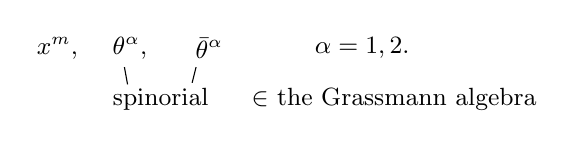
\begin{tikzpicture}[x=1cm,y=1cm,every node/.style={font=\small}]
\node at (0,0) {\(x^m,\)};
\node at (.92,0) {\(\theta^\alpha,\)};
\node at (1.93,0) {\(\bar\theta^\alpha\)};
\node at (3.87,0) {\(\alpha=1,2.\)};
\draw (.85,-.24) -- (.89,-.46);
\draw (1.76,-.24) -- (1.71,-.44);
\node[anchor=west] at (.58,-.65) {spinorial};
\node[anchor=west] at (2.34,-.65) {\(\in\) the Grassmann algebra};
\end{tikzpicture}}\endgroup}
\end{GelfandAdjacentEvidence}
\begin{GelfandAdjacentEvidence}{GELFAND-P000831}{6}

\[
\{\theta,\theta\}=0
\]
\Unclear{GELFAND-P000831}{new-variable-indices}{There is no discernible dot over the \(\alpha\) on \(\bar\theta\) in the list of variables.}
\end{GelfandAdjacentEvidence}
\begin{GelfandAdjacentEvidence}{GELFAND-P000831}{7}


\uwave{Functions on this space}:
\begin{equation*}
\begin{aligned}
\varphi(x,\theta,\bar\theta)
&=A(x)+\theta^\alpha\text{\sout{…}}\psi_\alpha(x)
+\bar\theta^{\dot\alpha}\bar\psi_{\dot\alpha}(x)
+\bar\theta_{\dot\alpha}\bar\theta^{\dot\alpha}C(x)+{}\\
&\quad+\theta^\alpha\theta_\alpha B(x)
+\theta\sigma^\alpha\bar\theta h_\alpha(x)
+\cdots+\theta^\alpha\theta_\alpha\bar\theta_{\dot\beta}\bar\theta^{\dot\beta}D(x)
\end{aligned}
\tag{4}
\end{equation*}
\Incomplete{GELFAND-P000831}{expansion-cancelled-field}{A sign is crossed out between \(\theta^\alpha\) and \(\psi_\alpha(x)\). It may be \(\varphi\) or \(\psi\).}
\end{GelfandAdjacentEvidence}
\begin{GelfandAdjacentEvidence}{GELFAND-P000831}{8}

\Unclear{GELFAND-P000831}{superfield-first-line}{A \(+\) occurs both at the end of the first manuscript line and at the start of the second.}
\end{GelfandAdjacentEvidence}
\begin{GelfandAdjacentEvidence}{GELFAND-P000831}{9}

\Unclear{GELFAND-P000831}{expansion-vector-index}{Both indices in \(\theta\sigma^\alpha\bar\theta h_\alpha(x)\) are provisionally read as \(\alpha\). The Latin \(a\) is possible.}
\end{GelfandAdjacentEvidence}
\begin{GelfandAdjacentEvidence}{GELFAND-P000831}{10}

\Unclear{GELFAND-P000831}{superfield-inserted-ellipsis}{The ellipsis before the last term is inserted from below with a caret.}
\end{GelfandAdjacentEvidence}
\begin{GelfandAdjacentEvidence}{GELFAND-P000831}{11}


There are 4 variables \(\theta\).

\uwave{Metric tensor} \(\varepsilon_{\alpha\beta}\)\textup{:}\quad
\(\varepsilon_{11}=\varepsilon_{22}=0,\qquad \varepsilon_{12}=-\varepsilon_{21}=1\)

Simplest \uwave{spinor representation}.
\Unclear{GELFAND-P000831}{spinor-representation-heading}{The Russian word for “simplest” may be abbreviated. The wavy underline begins at “spinor”.}
\end{GelfandAdjacentEvidence}
\begin{GelfandAdjacentEvidence}{GELFAND-P000831}{12}

\begin{equation*}
\left\{
\begin{aligned}
Q_\alpha&=-i\frac{\partial}{\partial\theta^\alpha}
-(\sigma^m\bar\theta)_\alpha\text{\sout{…}}\partial_m\\
\bar Q_{\dot\alpha}&=i\bar\partial_{\dot\alpha}
+(\theta\sigma^m)_{\dot\alpha}\partial_m
\end{aligned}
\right.
\tag{5}
\end{equation*}
\Incomplete{GELFAND-P000831}{operator-cancelled-mark}{Writing is visible between \((\sigma^m\bar\theta)_\alpha\) and \(\partial_m\) under a vertical zigzag. The original sign is illegible.}
\end{GelfandAdjacentEvidence}


\(\bar\partial_{\dot\alpha}\) — differentiation with respect to a Grassmann variable


\Needspace{7\baselineskip}
\begin{GelfandAdjacentEvidence}{GELFAND-P000832}{1}
\SourcePage{GELFAND-P000832}{unlabelled}
This realizes the system of commutation relations (1).

\uwave{Action of the group in superspace itself}.

(the action on functions is given)
\[
{x'}^m=x^m+c^m
\]
under supertranslations:
\begin{equation*}
\left\{\begin{aligned}
x^{m'}&=x^m+i(\theta\sigma^m\bar\lambda-\lambda\sigma^m\bar\theta)\\
\theta^{\alpha'}&=\theta^\alpha+\lambda^\alpha\\
\bar\theta^{\dot\alpha'}&=\bar\theta^{\dot\alpha}+\bar\lambda^{\dot\alpha}
\end{aligned}\right.
\tag{6}
\end{equation*}
\Unclear{GELFAND-P000832}{supertranslation-overwrite}{The first \(\theta\) on the right in the line for \(x^{m'}\) has been retraced. It reads \(\theta\). Any earlier sign is indiscernible.}
\end{GelfandAdjacentEvidence}
\begin{GelfandAdjacentEvidence}{GELFAND-P000832}{2}

\(\lambda,\bar\lambda\) — infinitesimal shifts of the Grassmann variables.

Perform the same transformation a second time with different parameters. We get a pure translation in \(x^m\).

Set:
\[
\delta_\lambda x^m=x^{m'}-x^m
=i(\theta\sigma^m\bar\lambda-\lambda\sigma^m\bar\theta)
\]
Then
\begin{equation*}
(\delta_\lambda\delta_\mu-\delta_\mu\delta_\lambda)x^m
=i(\mu\sigma^m\bar\lambda-\lambda\sigma^m\bar\mu)
\tag{7}
\end{equation*}
\Unclear{GELFAND-P000832}{commutator-coefficient}{The right-hand side has \(i\), with no visible \(2\) preceding it.}
\end{GelfandAdjacentEvidence}
\begin{GelfandAdjacentEvidence}{GELFAND-P000832}{3}


(i.e., a pure translation)

\uwave{Transformation law of the superfield}

\(\psi'(x')=\psi(x)\) — the ordinary transformation law of a scalar field

For supertranslations of the (scalar) superfield:
\begin{equation*}
\varphi'(x',\theta',\bar\theta')=\varphi(x,\theta,\bar\theta)
\tag{8}
\end{equation*}
For the fields \(A(x),\ldots\) from the expansion (4) this gives complicated formulas.

Consider some further new variables:
\begin{equation*}
\left\{\begin{aligned}
x_L^m&=x^m+i\theta\sigma^m\bar\theta\\
\delta x_L^m&=2i\theta\sigma^m\bar\lambda
\end{aligned}\right.
\qquad\delta\theta^\alpha=\lambda^\alpha
\tag{9}
\end{equation*}
(there is only \(\theta\) and no \(\bar\theta\))

Special fields (\textbf{chiral})
\Unclear{GELFAND-P000832}{chiral-word-inking}{The middle letters in the Russian word for “chiral” are retraced. The earlier strokes there cannot be distinguished.}
\end{GelfandAdjacentEvidence}
\begin{GelfandAdjacentEvidence}{GELFAND-P000832}{4}

\begin{equation*}
\varphi_L(x_L,\theta)=A(x_L)+\theta^\alpha\psi_\alpha(x_L)
+\theta^\alpha\theta_\alpha F(x_L)
\tag{10}
\end{equation*}
\Unclear{GELFAND-P000832}{chiral-field-symbol}{The field symbol is provisionally set as \(\varphi_L\). It may be \(\Phi_L\).}
\end{GelfandAdjacentEvidence}
\begin{GelfandAdjacentEvidence}{GELFAND-P000832}{5}

\Unclear{GELFAND-P000832}{chiral-final-argument}{The final \(x\) provisionally has subscript \(L\). Its lower stroke touches the closing parenthesis.}
\end{GelfandAdjacentEvidence}
\begin{GelfandAdjacentEvidence}{GELFAND-P000832}{6}

\begin{equation*}
\left\{\begin{aligned}
x_R^m&=x^m-i\theta\sigma^m\bar\theta\\
\delta x_{\underline{\underline R}}^m&=-2i\lambda\sigma^m\bar\theta
\end{aligned}\right.
\qquad\delta\bar\theta^{\dot\alpha}=\bar\lambda^{\dot\alpha}
\tag{11}
\end{equation*}
\Unclear{GELFAND-P000832}{right-index-double-underline}{The \(R\) in the line for \(\delta x_R^m\) is underlined twice.}
\end{GelfandAdjacentEvidence}



\Needspace{7\baselineskip}
\begin{GelfandAdjacentEvidence}{GELFAND-P000833}{1}
\SourcePage{GELFAND-P000833}{14}
We obtain.
\[
x^m=\frac12(x_L^m+x_R^m)
\]
\[
x_L^m-x_R^m=2i\theta\sigma^m\bar\theta
\]
\Unclear{GELFAND-P000833}{second-left-coordinate}{The initial \(x\) in the second formula has been retraced. The earlier strokes are indiscernible.}
\end{GelfandAdjacentEvidence}
\begin{GelfandAdjacentEvidence}{GELFAND-P000833}{2}

\Unclear{GELFAND-P000833}{post-formula-mark}{A faint trace to the right of \(\bar\theta\) lies along the paper ruling. It may be a full stop.}
\end{GelfandAdjacentEvidence}
\begin{GelfandAdjacentEvidence}{GELFAND-P000833}{3}


\SourceFigure{GELFAND-P000833}{dotted-divider}{%
\begingroup\color{black}\GelfandFitDiagram{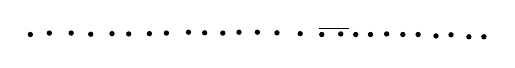
\begin{tikzpicture}[x=.36mm,y=.36mm]
\foreach \x/\y in {
0/0, 6.7/.5, 14.4/.5, 21.3/.1, 28.8/.3, 34.7/.2, 42.0/.3,
48.0/.5, 55.8/.8, 61.5/.6, 67.9/.5, 73.6/.8, 80.1/.8,
87.0/.6, 95.2/.3, 102.8/0, 109.5/.2, 114.8/0, 120.0/0,
125.7/.2, 131.4/0, 136.8/0, 143.1/-.5, 148.4/-.1, 154.7/-.8, 160.0/-.8}
  \fill (\x,\y) circle[radius=.34mm];
\draw[line width=.22pt] (101.8,2.3) -- (112.5,2.3);
\end{tikzpicture}}\endgroup\par
Divider of 26 dots. The fine horizontal stroke above the dots coincides with the paper ruling. Its relation to the divider is unclear.}
\end{GelfandAdjacentEvidence}



\Needspace{7\baselineskip}
\begin{GelfandAdjacentEvidence}{GELFAND-P000834}{1}
\SourcePage{GELFAND-P000834}{unlabelled}
\uline{26.3.79}\qquad \uline{Gelfand Sem.}

\SourceFigure{GELFAND-P000834}{date-underline-marks}{%
\begingroup\color{black}\GelfandFitDiagram{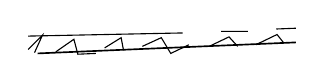
\begin{tikzpicture}[x=1cm,y=1cm]
\draw (0,.24) -- (1.96,.28) (2.45,.30) -- (2.79,.30)
      (3.15,.33) -- (3.40,.34);
\draw[semithick] (.12,.02) -- (3.40,.16);
\draw (0,.07)--(.18,.25)--(.08,.03)
  (.35,.04)--(.58,.20)--(.63,.01)--(.86,.02)
  (.97,.09)--(1.18,.22)--(1.21,.06)
  (1.45,.11)--(1.69,.22)--(1.81,.02)--(2.04,.13)
  (2.32,.12)--(2.55,.23)--(2.66,.11)
  (2.89,.13)--(3.16,.26)--(3.24,.16);
\end{tikzpicture}}\endgroup\par
Overlapping horizontal and angular strokes appear below the date. No individual letters can be made out.}
\end{GelfandAdjacentEvidence}
\begin{GelfandAdjacentEvidence}{GELFAND-P000834}{2}


\uuline{Lebedev (Mitya)}

\uwave{On results of Ritt and Kirillov in differential algebra}.

\(M\) — a smooth manifold, \(\dim M=n\)

\SourceFigure{GELFAND-P000834}{vector-bundle-arrow}{%
\begingroup\color{black}\GelfandFitDiagram{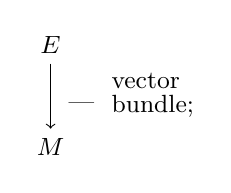
\begin{tikzpicture}[x=1cm,y=1cm,every node/.style={font=\small}]
\node (e) at (0,.63) {\(E\)};
\node (m) at (0,-.66) {\(M\)};
\draw[->] (e)--(m);
\node[anchor=west] at (.65,.18) {vector};
\node[anchor=west] at (.65,-.14) {bundle;};
\node at (.39,-.12) {—};
\end{tikzpicture}}\endgroup}
\end{GelfandAdjacentEvidence}
\begin{GelfandAdjacentEvidence}{GELFAND-P000834}{3}


\(\Gamma^\infty(E)\) — smooth sections.
\[
s_1,s_2\in\Gamma^\infty(E)
\]
Introduce a bilinear operation: \([\cdot,\cdot]\):
\[
[s_1,s_2]\in\Gamma^\infty(E)
\]
\Unclear{GELFAND-P000834}{bracket-result-membership}{The sign before \(\Gamma^\infty(E)\) is retraced and provisionally read as \(\in\).}
\end{GelfandAdjacentEvidence}
\begin{GelfandAdjacentEvidence}{GELFAND-P000834}{4}


a) bilin., skew-symm., Jacobi id.

b) cont. in the topol. of unif. conv. of derivs. on compact sets

\Unclear{GELFAND-P000834}{continuity-abbreviation}{The Russian abbreviation for convergence provisionally reads «схд.». A separate «о» may be present between «х» and the retraced «д».}
\end{GelfandAdjacentEvidence}
\begin{GelfandAdjacentEvidence}{GELFAND-P000834}{5}


c) \(\operatorname{supp}[s_1,s_2]\subset
\operatorname{supp}s_1\cap\operatorname{supp}s_2\)
\qquad (locality)

[crossed out: \sout{…}] This is called a \uwave{differential Lie algebra}.
\Incomplete{GELFAND-P000834}{cancelled-final-word}{The beginning of the crossed-out fragment has a loop resembling «В». The remaining letters are illegible.}
\end{GelfandAdjacentEvidence}



\Needspace{7\baselineskip}
\begin{GelfandAdjacentEvidence}{GELFAND-P000835}{1}
\SourcePage{GELFAND-P000835}{20}
\uwave{The same definition in loc. coordinates}

Let \(F\) — the fiber; \(\dim F=1\)

\(x_1,\ldots,x_n\) — coords. on the base.

Then locally
\begin{equation*}
[f,g]=\sum c_{k\ell}(x)\partial^k f\cdot\partial^\ell g,
\qquad k,\ell\text{ — multi-indices}
\tag{1}
\end{equation*}
\uwave{Kirillov's main result}: classification of such algebras.

\uline{Theorem 1}. All loc. algebras with a fiber of dim. 1 are exhausted by two (essentially)

\begin{equation*}
\text{a)}\quad M=\mathbb R^{2n},\qquad
[f,g]=\sum\left(\frac{\partial f}{\partial x_i}\frac{\partial g}{\partial y_i}
-\frac{\partial f}{\partial y_i}\frac{\partial g}{\partial x_i}\right)
\tag{2}
\end{equation*}
\Unclear{GELFAND-P000835}{poisson-overwriting}{Overlapping strokes appear in the first numerator with \(g\) and the second denominator with \(y_i\). The earlier letter forms cannot be distinguished.}
\end{GelfandAdjacentEvidence}
\begin{GelfandAdjacentEvidence}{GELFAND-P000835}{2}


\begin{equation*}
\begin{gathered}
\text{b)}\quad M=\mathbb R^{2n+1},\quad
X_i=\frac{\partial}{\partial x_i},\quad
Y_i=\frac{\partial}{\partial y_i}+x_i\frac{\partial}{\partial z},\quad
Z=\frac{\partial}{\partial z}\text{ — vect. fields}
\end{gathered}
\tag{3}
\end{equation*}
\Unclear{GELFAND-P000835}{contact-vector-sign}{A plus is visible before \(x_i\partial/\partial z\) in the entry for \(Y_i\).}
\end{GelfandAdjacentEvidence}
\begin{GelfandAdjacentEvidence}{GELFAND-P000835}{3}

\begin{equation*}
[f,g]=fZg-gZf+\sum_{i=1}^{n}(X_i f\cdot Y_i g-X_i g\cdot Y_i f)
\tag*{$(3)_1$}
\end{equation*}
\Unclear{GELFAND-P000835}{contact-bracket-sign}{A plus is visible before the sum in \((3)_1\).}
\end{GelfandAdjacentEvidence}
\begin{GelfandAdjacentEvidence}{GELFAND-P000835}{4}

All the others are formally isomorphic to them.

\uline{Ritt}.

\uwave{Differential Lie group and diff. Lie algebra}.

\SourceFigure{GELFAND-P000835}{dimension-diagram}{%
\begingroup\color{black}\GelfandFitDiagram{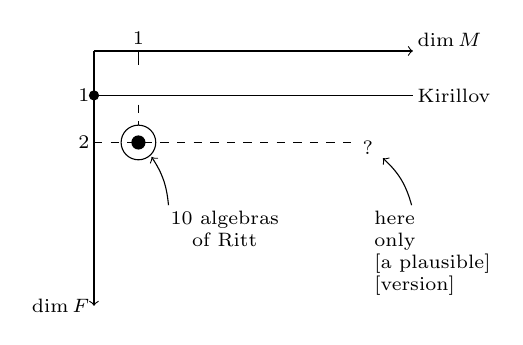
\begin{tikzpicture}[x=.83cm,y=.83cm,every node/.style={font=\scriptsize,inner sep=1.5pt}]
\draw[->] (0,0)--(4.88,0) node[above right] {\(\dim M\)};
\draw[->] (0,0)--(0,-3.9) node[left] {\(\dim F\)};
\draw (.68,.01)--(.68,-.22);
\node[above] at (.68,.03) {1};
\node[left] at (0,-.68) {1};
\node[left] at (0,-1.4) {2};
\draw (0,-.68)--(4.88,-.68) node[right] {Kirillov};
\fill (0,-.68) circle[radius=.065cm];
\draw[dashed] (0,-1.4)--(4.03,-1.4);
\draw[dashed] (.68,-.82)--(.68,-1.14);
\draw (.68,-1.4) circle[radius=.22cm];
\fill (.68,-1.4) circle[radius=.09cm];
\node[below] at (4.19,-1.31) {?};
\draw[->] (1.14,-2.36) to[bend right=14] (.88,-1.62);
\draw[->] (4.86,-2.36) to[bend right=16] (4.42,-1.64);
\node[align=center,below] at (2.0,-2.37) {10 algebras\\of Ritt};
\node[align=left,below] at (5.18,-2.37) {here\\only\\\relax [a plausible]\\\relax [version]};
\end{tikzpicture}}\endgroup\par
At the right margin. The last two lines at the right are provisionally read as «правдопод. / версия» (“plausible / version”).}
\end{GelfandAdjacentEvidence}
\begin{GelfandAdjacentEvidence}{GELFAND-P000835}{5}


Consider series
\begin{equation*}
\sigma_1=\sum_{i\ge 1}a_i\,a\,\xi^{-(i+1)}
\tag{4}
\end{equation*}
\Unclear{GELFAND-P000835}{series-extra-mark}{A separate dark sign resembling \(a\) occurs between \(a_i\) and \(\xi\).}
\end{GelfandAdjacentEvidence}
\begin{GelfandAdjacentEvidence}{GELFAND-P000835}{6}


[crossed out: \sout{…}] and the commutator
\Incomplete{GELFAND-P000835}{cancelled-before-commutator}{A short entry at the left is crossed out. The underlying marks are illegible.}
\end{GelfandAdjacentEvidence}
\begin{GelfandAdjacentEvidence}{GELFAND-P000835}{7}

\begin{equation*}
[\sigma_1,\sigma_2]=\sigma_1\cdot\sigma_2-\sigma_2\cdot\sigma_1
\tag{5}
\end{equation*}
(here \(\dim M=1\), \(\dim F=\infty\)).

\([\xi,x]=1\) — this determines everything.

\SourceFigure{GELFAND-P000835}{double-divider}{%
\begingroup\color{black}\GelfandFitDiagram{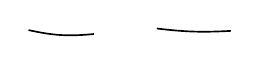
\begin{tikzpicture}
\draw[semithick] (0,0) to[bend right=9] (.83,-.05);
\draw[semithick] (1.63,.02) to[bend right=5] (2.57,-.01);
\end{tikzpicture}}\endgroup}
\end{GelfandAdjacentEvidence}
\begin{GelfandAdjacentEvidence}{GELFAND-P000835}{8}


\(\mathcal F\) — diff. field of char. \(0\), \qquad “\(\partial=\frac{\partial}{\partial x}\)”

\(y_1(x),\ldots,y_n(x)\) — diff. independent

Consider the ring
\begin{equation*}
\mathcal F[[y_i^{(j)}]]\simeq\bigoplus\mathcal F_\tau,
\qquad \tau\text{ — “order” — degree — number of factors}
\tag{6}
\end{equation*}
\Unclear{GELFAND-P000835}{ring-grading}{The relation sign has a wavy upper stroke and is provisionally set as \(\simeq\). The index is provisionally read as \(\tau\).}
\end{GelfandAdjacentEvidence}
\begin{GelfandAdjacentEvidence}{GELFAND-P000835}{9}


\uwave{Formal diff. Lie group} \(\equiv\) form. group law \(\equiv\) set of fns.
\begin{equation*}
U_i\in\mathcal F[[u_i^{(j)},v_\ell^{(m)}]]
\tag{7}
\end{equation*}
\Unclear{GELFAND-P000835}{differential-variables}{A short horizontal stroke at the upper right of \(v\) is joined to the letter. It may be a separate bar.}
\end{GelfandAdjacentEvidence}


Satisfies 2 axioms:

a) \(U_i(\bar u,0)=\bar u_i,\qquad U_i(0,\bar v)=\bar v_i\)

b) associativity.


\Needspace{7\baselineskip}
\begin{GelfandAdjacentEvidence}{GELFAND-P000836}{1}
\SourcePage{GELFAND-P000836}{unlabelled}
\uline{Example}.

\SourceFigure{GELFAND-P000836}{taylor-vertical-relation}{%
\begingroup\color{black}\GelfandFitDiagram{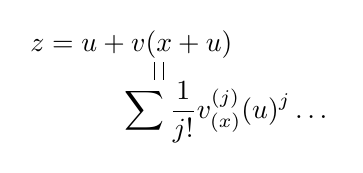
\begin{tikzpicture}[x=1cm,y=1cm,every node/.style={inner sep=1pt}]
\node[anchor=west] at (0,0) {\(z=u+v(x+u)\)};
\draw (1.62,-.23)--(1.62,-.45) (1.73,-.23)--(1.73,-.45);
\node[anchor=west] at (1.20,-.86)
  {\(\displaystyle\sum\frac{1}{j!}v^{(j)}_{(x)}(u)^j\,\text{\sout{…}}\)};
\end{tikzpicture}}\endgroup\par
Below \(v(x+u)\), two vertical strokes stand between the formula and the series.}
\end{GelfandAdjacentEvidence}
\begin{GelfandAdjacentEvidence}{GELFAND-P000836}{2}

\Unclear{GELFAND-P000836}{expansion-cancel}{A further entry after \((u)^j\) is crossed out. It may read \(u^j\).}
\end{GelfandAdjacentEvidence}
\begin{GelfandAdjacentEvidence}{GELFAND-P000836}{3}


(for the group of diffeomorphisms, leav. \(\downarrow x\) in place)
\Unclear{GELFAND-P000836}{diffeomorphism-mark}{A short vertical stroke occurs between the Russian abbreviation «ост.» and \(x\). It is provisionally rendered as a downward arrow.}
\end{GelfandAdjacentEvidence}
\begin{GelfandAdjacentEvidence}{GELFAND-P000836}{4}


Form. series:
\[
\begin{aligned}
U&=\sum_{k=0}^{\infty}P_k,\\
P_k&=\text{homog. polyn. of deg. }k\text{ in }
u_1,\ldots,u_n,u_1^{(1)},\ldots,u_n^{(1)},
\end{aligned}
\]
over a diff. field (a field of functions with diff.)
\Unclear{GELFAND-P000836}{formal-overwrite}{The start of the Russian word for “functions” is overwritten. Its earlier form is illegible.}
\end{GelfandAdjacentEvidence}
\begin{GelfandAdjacentEvidence}{GELFAND-P000836}{5}


\uline{Theorem} 2

\uwave{Classific. of diff. groups with a fiber of dim.} 2

\(A^h.\)
\SourceFigure{GELFAND-P000836}{group-operation-callout}{%
\begingroup\color{black}\GelfandFitDiagram{\begin{tikzpicture}[x=1cm,y=1cm,every node/.style={inner sep=1pt}]
\node at (0,0) {\(u(x)\,dx^{-h}+v(x)\,dx^{-h}\)};
\draw[->] (-.17,-.66)--(-.10,-.27);
\node[align=center,below,font=\small] at (-.13,-.70)
  {operation\\in the group};
\end{tikzpicture}}\endgroup}
\end{GelfandAdjacentEvidence}

\[
u\circ v=u+v
\]
\[
\Pi:\qquad u\circ v=u+v(x+u)
\]
All groups are ext. of \(\Pi\) by \(A^h\).


\Needspace{7\baselineskip}
\begin{GelfandAdjacentEvidence}{GELFAND-P000837}{1}
\SourcePage{GELFAND-P000837}{unlabelled}
\uline{2/IV–78}\qquad \uline{Gelfand Sem.}
\Unclear{GELFAND-P000837}{date-year}{The last digit of the year is provisionally read as 8. It may be 9.}
\end{GelfandAdjacentEvidence}
\begin{GelfandAdjacentEvidence}{GELFAND-P000837}{2}


\uline{K. Shabat}. \quad From the work of \uwave{Griffiths and Chern}.
\Unclear{GELFAND-P000837}{speaker-initial}{The initial is provisionally read as the Russian «К.». It may be «Ю.».}
\end{GelfandAdjacentEvidence}
\begin{GelfandAdjacentEvidence}{GELFAND-P000837}{3}


A web — a finite number of foliations with transv. leaves. It is constructed \uline{on} a manifold.

(net) — \uline{Web}

\[
X\subset P^n,\qquad \dim X=m,\qquad \operatorname{deg}X=d.
\]
[Below \(X\):] proj. set (algebr.)

A web in \(\mathrm{Gr}(m,n-m)\), more precisely in some open subset of it:
\Unclear{GELFAND-P000837}{grassmann-qualifier}{The Russian phrase between “in” and “open” provisionally reads «нек. его» (“some … of it”). The middle is faint.}
\end{GelfandAdjacentEvidence}
\begin{GelfandAdjacentEvidence}{GELFAND-P000837}{4}


\begin{equation*}
U=\{H\mid H\cdot X=d\text{ distinct points}\}
\quad\text{— an open set}
\tag{1}
\end{equation*}

\SourceFigure{GELFAND-P000837}{curve-line-intersections}{%
\begingroup\color{black}\GelfandFitDiagram{\begin{tikzpicture}[x=1cm,y=1cm,line width=.65pt]
\draw (-.35,-1.15)--(.43,1.35);
\draw (.88,.66) .. controls (.68,.82) and (.46,.90) .. (.29,.83)
 .. controls (-.23,.72) and (-.48,.29) .. (-.01,.18)
 .. controls (.45,.23) and (.84,.09) .. (.78,-.28)
 .. controls (.73,-.68) and (.28,-.61) .. (-.20,-.66)
 .. controls (-.45,-.69) and (-.61,-.63) .. (-.79,-.63);
\draw[line width=1.35pt] (-.78,-.63)--(-.20,-.66);
\fill (.29,.83) circle[radius=.072cm];
\fill (.065,.18) circle[radius=.072cm];
\fill (-.20,-.66) circle[radius=.086cm];
\end{tikzpicture}}\endgroup}
\end{GelfandAdjacentEvidence}
\begin{GelfandAdjacentEvidence}{GELFAND-P000837}{5}


([crossed out: \sout{…}] when there is multiplicity, discard it)
\Incomplete{GELFAND-P000837}{multiplicity-cancel}{The first word inside the parentheses is crossed out. Its letters are indiscernible.}
\end{GelfandAdjacentEvidence}
\begin{GelfandAdjacentEvidence}{GELFAND-P000837}{6}


\uline{I.M.G.}

\uwave{Crofton's formula}: length of a curve = average number of points at which a line intersects it
(average over lines with respect to an invariant measure).

Griffiths and Chern, inspired by Penrose's work, generalized this to the multidimensional [inserted below at left: \(\leftarrow\) case].
\Unclear{GELFAND-P000837}{multidimensional-insertion}{The word “case” is below the line at the left. A short arrow above it points left.}
\end{GelfandAdjacentEvidence}
\begin{GelfandAdjacentEvidence}{GELFAND-P000837}{7}


\uwave{The leaf passing through the point} \(H_0\in U\), \uwave{consists of}
[crossed out: \sout{surfaces}].
\Unclear{GELFAND-P000837}{slice-cancel-right}{The crossed-out Russian word is provisionally read as «поверхностей» (“surfaces”).}
\end{GelfandAdjacentEvidence}
\begin{GelfandAdjacentEvidence}{GELFAND-P000837}{8}


[crossed out: \sout{points of \(X\)}] \uwave{planes}
\[
\{H\in U\mid \exists i\in\{1,2,\ldots,d\};\ \underline{P}_i\in H\}.
\]
\Unclear{GELFAND-P000837}{slice-cancel-left}{“Points of \(X\)” is crossed out at the start of the line. There is a short stroke below the first \(P_i\).}
\end{GelfandAdjacentEvidence}
\begin{GelfandAdjacentEvidence}{GELFAND-P000837}{9}

\[
H_0\cdot X=P_1+\ldots+P_d
\]
\begin{equation*}
\{H\in U\mid \exists i\in\{1,2,\ldots,d\},\ P_i\in H\}
\tag{2}
\end{equation*}

This is a foliation of codimension 1. (so here the planes are div. into leaves, they themselves can intersect)
\Unclear{GELFAND-P000837}{foliation-note}{The Russian abbreviations provisionally read «зд.» (“here”) and «разд.» (“div.”).}
\end{GelfandAdjacentEvidence}
\begin{GelfandAdjacentEvidence}{GELFAND-P000837}{10}


\uline{I.M.G.}\quad [crossed out: \sout{Questions}]
\Unclear{GELFAND-P000837}{problem-cancel}{The crossed-out word provisionally reads «Вопросы» (“Questions”).}
\end{GelfandAdjacentEvidence}
\begin{GelfandAdjacentEvidence}{GELFAND-P000837}{11}


\uline{Problem}: \uwave{there are 3 foliations} (transv.) When can they be straightened?
[Inserted below “there are 3 foliations”:] \uwave{in the plane}.

(2 always!!)

3 can be straightened \(\Leftrightarrow\) it is hexagonal, i.e.

\(\approx1927\) 

\SourceFigure{GELFAND-P000837}{hexagonal-path}{%
\begingroup\color{black}\GelfandFitDiagram{\begin{tikzpicture}[x=1cm,y=1cm,line width=.62pt]
\draw (-1.45,.07)--(-1.16,.12)--(-.95,.05)--(-.39,.08)--(0,0)
      --(.70,-.08)--(1.34,-.17);
\draw (-.61,1.22)--(-.26,.57)--(0,0)--(.38,-.56)--(.55,-.88);
\draw[->] (.98,.97)--(.51,.55)--(0,0)--(-.53,-.52)--(-1.18,-1.22);
\draw[line width=.8pt] (-.95,.05)--(-.26,.57)--(.51,.55);
\draw[line width=.8pt] (-.95,.05)--(-.53,-.52)--(.38,-.56)--(.70,-.08);
\fill (-1.45,.07) circle[radius=.046cm];
\fill (-.26,.57) circle[radius=.060cm];
\draw (.51,.55) circle[radius=.09cm];
\draw (-.95,.05) circle[radius=.068cm];
\draw (-.53,-.52) circle[radius=.065cm];
\fill (.38,-.56) circle[radius=.052cm];
\fill (0,0) circle[radius=.075cm];
\fill (.70,.037)--(.83,-.08)--(.70,-.21)--(.61,-.08)--cycle;
\fill (-.32,1.05) circle[radius=.032cm];
\end{tikzpicture}}\endgroup\par
The redraw follows the visible lines, small circles and thickened nodes. The order of traversal and the direction of some small arrows are indistinct.}
\end{GelfandAdjacentEvidence}
\begin{GelfandAdjacentEvidence}{GELFAND-P000837}{12}


— such a path (infinitesimal) must be closed. — something like curvature.

\SourceFigure{GELFAND-P000837}{separate-footer-strokes}{%
\begingroup\color{black}\GelfandFitDiagram{\begin{tikzpicture}
\fill (0,0) circle[radius=.038cm];
\draw (0,0) to[bend right=5] (.45,-.02) -- (1.35,0);
\draw (2.05,.04) -- (3.35,.16);
\end{tikzpicture}}\endgroup}
\end{GelfandAdjacentEvidence}



\Needspace{7\baselineskip}
\begin{GelfandAdjacentEvidence}{GELFAND-P000838}{1}
\SourcePage{GELFAND-P000838}{29}
Now \(m=1\).
\[
\begin{array}{@{}l@{}}
X\subset P^n\\[-.15em]
\vert\\[-.15em]
\text{proj. \uwave{curve}}
\end{array}
\]

\(\check P^n\) — dual proj. space.
\begin{equation*}
\check{\mathbb P}^{\,n}\supset U
=\{H\mid H\circ X=d\text{ distinct points}\}
\tag{3}
\end{equation*}
\Unclear{GELFAND-P000838}{intersection-sign}{A small oval is visible between \(H\) and \(X\), provisionally set as \(\circ\).}
\end{GelfandAdjacentEvidence}
\begin{GelfandAdjacentEvidence}{GELFAND-P000838}{2}


On \(U\) we get a web of codimension 1.

\SourceFigure{GELFAND-P000838}{pencil-diagram}{%
\begingroup\color{black}\GelfandFitDiagram{\begin{tikzpicture}[x=.019cm,y=-.019cm,line cap=round,line width=.5pt]
\coordinate (a) at (154,56);
\coordinate (b) at (123,112);
\coordinate (c) at (98,177);
\draw[line width=.85pt] (197,77) .. controls (177,55) and (168,53) .. (a)
 .. controls (101,49) and (59,103) .. (b)
 .. controls (160,111) and (176,130) .. (172,150)
 .. controls (164,168) and (140,173) .. (c) -- (47,174);
\draw (112,33)--(a)--(193,83) (138,23) .. controls (145,27) and (151,46) .. (a)
 -- (170,101) (167,30)--(a)--(b)--(c)--(90,201);
\draw (205,26)--(a)--(119,77) (213,37)--(a)--(105,76);
\draw (105,92)--(b) .. controls (131,120) and (137,127) .. (140,141);
\draw (121,90)--(b)--(122,147) (77,123)--(b)--(165,103)
 (88,134)--(b)--(147,96);
\draw (51,196)--(c)--(135,159) (48,213)--(c)--(129,152)
 (90,147)--(c)--(104,216) (73,157) .. controls (84,151) and (93,171) .. (c)
 -- (113,201);
\fill (a) circle[radius=.066cm];
\fill (b) circle[radius=.066cm];
\fill (c) circle[radius=.071cm];
\end{tikzpicture}}\endgroup\par
The redraw follows the three centers and the discernible strokes. Some strokes merge, so their exact number is uncertain.}
\end{GelfandAdjacentEvidence}
\begin{GelfandAdjacentEvidence}{GELFAND-P000838}{3}


\uwave{Abelian eq. for the web}.

\SourceFigure{GELFAND-P000838}{grid-geometry}{%
\begingroup\color{black}\GelfandFitDiagram{\begin{tikzpicture}[x=.016cm,y=-.016cm,line width=.55pt]
\draw (120,72) .. controls (128,33) and (165,18) .. (191,20)
 .. controls (218,22) and (233,50) .. (230,72)
 .. controls (227,101) and (205,130) .. (170,136)
 .. controls (132,145) and (109,121) .. (120,72);
\draw (152,57) .. controls (180,52) and (178,93) .. (179,128);
\draw (190,47) .. controls (204,58) and (205,96) .. (203,116);
\draw (217,45) .. controls (228,38) and (230,86) .. (234,106);
\draw (140,97) .. controls (164,73) and (211,56) .. (252,38);
\draw (150,108) .. controls (192,91) and (219,78) .. (246,67);
\draw (156,129) .. controls (178,116) and (203,111) .. (229,102);
\node[anchor=west,font=\small] at (19,42) {\([u]\)};
\end{tikzpicture}}\endgroup}
\end{GelfandAdjacentEvidence}
\begin{GelfandAdjacentEvidence}{GELFAND-P000838}{4}

\Unclear{GELFAND-P000838}{grid-label}{The sign to the left of the oval is provisionally set as \(u\). It may be \(U\).}
\end{GelfandAdjacentEvidence}
\begin{GelfandAdjacentEvidence}{GELFAND-P000838}{5}


\begin{equation*}
\begin{cases}
u_1=\mathrm{const}.\\
\vdots\\
u_n=\mathrm{const}
\end{cases}
\tag{4}
\end{equation*}

\uwave{The Ab. eq. for the web has the form}:
\begin{equation*}
\sum_{i=1}^{d}f_i(u_i)\,du_i=0,\qquad
\sum_{i=1}^{d}f_i(u_i)\,du_i\in\Omega^1(U)
\tag{5}
\end{equation*}

There is a dependence among the normal vectors (cotang. vectors), and the coefficients have the form \(f_i(u_i)\).

\uline{Rank of the web} \(\underset{\mathrm{def}}{=}\)
\uwave{max. number of lin. independent Abelian eqs.}, \uwave{that it satisfies}.

\uuline{Prop. 1}
\uwave{The rank of the web constructed from a curve of genus} \(g\), \uwave{equals} \(g\).

[crossed out: \sout{Another theorem 1 — Under the conditions}
\sout{\(n\ge3,\ d\ge2n\)}]
\Unclear{GELFAND-P000838}{cancelled-heading}{The first crossed-out word provisionally reads «Еще» (“Another”).}
\end{GelfandAdjacentEvidence}
\begin{GelfandAdjacentEvidence}{GELFAND-P000838}{6}

\Unclear{GELFAND-P000838}{cancelled-hypotheses}{The crossed-out conditions provisionally read \(n\ge3,\ d\ge2n\).}
\end{GelfandAdjacentEvidence}
\begin{GelfandAdjacentEvidence}{GELFAND-P000838}{7}


\uline{Theorem} 1 (Chern, 193 ?)
\Unclear{GELFAND-P000838}{chern-year}{A question mark follows 193 in the manuscript.}
\end{GelfandAdjacentEvidence}
\begin{GelfandAdjacentEvidence}{GELFAND-P000838}{8}


\SourceFigure{GELFAND-P000838}{rank-callouts}{%
\begingroup\color{black}\GelfandFitDiagram{\begin{tikzpicture}[x=1cm,y=1cm,every node/.style={font=\small}]
\node[anchor=west] at (0,0) {\uwave{Rank of the \(d\)-web}};
\node[anchor=west] at (3.65,0) {\(\le\pi(n,d)\)};
\draw[->] (.10,-1.32)--(.61,-.29);
\node[anchor=west,align=left] at (0,-1.53) {(arbitr. web!)};
\node[anchor=west,align=left] at (1.25,-.90) {(\uwave{in an \(n\)-dim.}\\\uwave{set})};
\node[anchor=west,align=left] at (3.65,-.40) {(Castelnuovo number)};
\end{tikzpicture}}\endgroup}
\end{GelfandAdjacentEvidence}


\begin{equation*}
\pi(n,d)\underset{\mathrm{def}}{=}
\text{max. genus of a curve of degree }d\text{ in }\mathbb P^n,
\qquad \underline{\underline{n,d\ge2}}.
\tag{6}
\end{equation*}

There is a short formula
\begin{equation*}
\pi(n,d)=m\left(d-\frac12(m+1)(n-1)-1\right),
\quad\text{where }m=\left[\frac{d-1}{n-1}\right].
\tag{7}
\end{equation*}


\Needspace{7\baselineskip}
\begin{GelfandAdjacentEvidence}{GELFAND-P000839}{1}
\SourcePage{GELFAND-P000839}{unlabelled}
\uuline{Theorem 2.}

(main)

\uwave{If} \(n\ge3,\ d\ge2n\) and \uwave{the \(d\)-web has rank} \(\pi(n,d)\),

\uwave{then}

1) \uwave{It can be linearized}

2) \uwave{It extends to a web obtained from} \(X\subset\mathbb P^n\).

The connection between such eqs. and Abelian differentials is explained.

\uline{Reference:}

\uwave{(Sonderdruck aus) Jber. d. Dt. Math.-Verein}, \(80\) (\(1978\)), 13–110

[Under «Sonderdruck aus»: \uwave{offprint} from.]

(Jahresberichte der Deutsche[…] Math. Vereinigung)
\Unclear{GELFAND-P000839}{reference-expansion}{The ending after “Deutsche” is uncertain. “Deutschen” and “Deutscher” are possible.}
\end{GelfandAdjacentEvidence}
\begin{GelfandAdjacentEvidence}{GELFAND-P000839}{2}


[crossed out: \sout{…}]
\Incomplete{GELFAND-P000839}{reference-cancelled-word}{A word below the reference is crossed out. Its initial loop is visible, and the remaining letters are obscured.}
\end{GelfandAdjacentEvidence}
\begin{GelfandAdjacentEvidence}{GELFAND-P000839}{3}


A geometry is being developed for
\SourceFigure{GELFAND-P000839}{projective-connection-underlining}{%
\begingroup\color{black}\GelfandFitDiagram{\begin{tikzpicture}[x=1cm,y=1cm,every node/.style={inner sep=1pt}]
\node[anchor=west] at (0,0) {projective connections.};
\draw[->] (.93,-.28)--(0,-.28);
\draw (1.70,-.28)--(3.89,-.28);
\end{tikzpicture}}\endgroup\par
The left stroke has a left-pointing arrow. A separate stroke runs under the words at right.}
\end{GelfandAdjacentEvidence}
\begin{GelfandAdjacentEvidence}{GELFAND-P000839}{4}


\uline{Zamolodchikov A.} (Sasha) \quad Suppose there is \(S_{ij}^{k\ell}(\lambda)\)
\Unclear{GELFAND-P000839}{initial-matrix-indices}{The upper indices are provisionally read as \(k,\ell\). They touch the stroke from the preceding line.}
\end{GelfandAdjacentEvidence}
\begin{GelfandAdjacentEvidence}{GELFAND-P000839}{5}


Suppose there is also a picture:

\(L\) lines, angles \(\lambda_1,\ldots,\lambda_L\)

\(\lambda_i\) in increasing order

(from some line

[crossed out: \sout{Then}]
\Unclear{GELFAND-P000839}{cancelled-to}{The crossed-out word provisionally reads «То» (“Then”).}
\end{GelfandAdjacentEvidence}
\begin{GelfandAdjacentEvidence}{GELFAND-P000839}{6}


\SourceFigure{GELFAND-P000839}{single-vertex-diagram}{%
\begingroup\color{black}\GelfandFitDiagram{\begin{tikzpicture}[x=1cm,y=1cm,line width=.72pt]
\draw (-.72,.85)--(.04,0)--(.75,-.77);
\draw (.95,.79)--(.04,0)--(-.70,-.65);
\draw[->,thick] (.39,-.38)--(.60,-.62);
\draw[->,thick] (-.23,-.24)--(-.61,-.58);
\draw (.04,0) circle[radius=.083cm];
\node at (-.58,1.04) {\([c]\)};
\node at (1.20,.75) {\(j\)};
\node at (-.62,-.95) {\(i\)};
\node at (1.25,-.42) {\(k\)};
\end{tikzpicture}}\endgroup\par
The upper-left sign resembles \(c\) and may be \(\ell\).}
\end{GelfandAdjacentEvidence}
\begin{GelfandAdjacentEvidence}{GELFAND-P000839}{7}


indices \(=1,2,\ldots,N\)

\SourceFigure{GELFAND-P000839}{many-lines-diagram}{%
\begingroup\color{black}\GelfandFitDiagram{\begin{tikzpicture}[x=.013cm,y=-.013cm,line width=.65pt]
\draw (12,181) .. controls (86,175) and (121,172) .. (168,174)
 .. controls (222,175) and (270,182) .. (325,176);
\draw (40,256) .. controls (60,218) and (68,211) .. (86,178)
 -- (133,116)--(166,81)--(237,14);
\draw (76,12)--(100,51)--(133,116)--(166,172)
 .. controls (177,200) and (185,224) .. (193,251);
\draw (31,21) .. controls (46,21) and (78,40) .. (100,51)
 -- (166,81) .. controls (208,105) and (249,151) .. (280,179)
 -- (360,241);
\draw (228,22)--(238,15)--(234,25)
 (47,247)--(40,256)--(49,251)
 (355,233)--(360,241)--(352,237);
\foreach \x/\y/\r in {100/51/7,166/81/6,133/116/6,86/178/7,166/172/7,280/179/9}
  \draw (\x,\y) circle[radius=\r];
\end{tikzpicture}}\endgroup\par
There are six circled intersections. Short strokes at the ends are drawn as visible. Some arrow directions are unclear.}
\end{GelfandAdjacentEvidence}
\begin{GelfandAdjacentEvidence}{GELFAND-P000839}{8}


To a node — a matrix; to tails — indices, I sum over the links.

We get a matrix (large). What is its behavior as \(L\to\infty\)?
\[
Z^{j_1\ldots j_L}_{i_1\ldots i_L}(\lambda_1,\ldots,\lambda_L).
\]

\uline{Problem 1.} There is an asymptotic formula

(how to calc. it exactly — unknown)
\Unclear{GELFAND-P000839}{problem-parenthesis}{The Russian words provisionally read «сосч. точно» (“calculate exactly”). «сосч. её» (“calculate it”) is possible.}
\end{GelfandAdjacentEvidence}
\begin{GelfandAdjacentEvidence}{GELFAND-P000839}{9}

\begin{equation*}
\ln Z\text{\sout{…}}\sim\text{proport. to the number of nodes}
\tag{1}
\end{equation*}
\Unclear{GELFAND-P000839}{hatched-indices}{After \(Z\) the hatching covers signs resembling the indices \(j_1\ldots j_L,\ i_1\ldots i_L\) and arguments \((\lambda_1,\ldots,\lambda_L)\). Some of the signs cannot be made out.}
\end{GelfandAdjacentEvidence}
\begin{GelfandAdjacentEvidence}{GELFAND-P000839}{10}


\begin{equation*}
Z\underset{\mathrm{df}}{=}Z^{i_1\ldots i_L}_{i_1\ldots i_L}
\qquad\text{(“trace”)}\qquad\text{(sum over repeated indices)}
\tag{2}
\end{equation*}
Each line \(\leadsto\) parameter \(\lambda_j\)

(the rays are numbered clockwise \uwave{\(i_1,\ldots,i_L,j_1,\ldots,j_L\)}.)
\Unclear{GELFAND-P000839}{clockwise-indices}{The first subscripts on \(i\) and \(j\) are provisionally set as the digit \(1\). Their shapes also resemble \(L\).}
\end{GelfandAdjacentEvidence}
\begin{GelfandAdjacentEvidence}{GELFAND-P000839}{11}


\begin{equation*}
Z^{j_1\ldots j_L}_{i_1\ldots i_L}
=\sum_{\substack{\text{internal}\\\text{\sout{…}}\\\text{segments}}}
\left(\prod_{\substack{\text{points of}\\\text{intersection}}}
S^{**}_{**}(\lambda_a-\lambda_b)\right)
\tag{3}
\end{equation*}
\Incomplete{GELFAND-P000839}{sum-cancelled-word}{The middle line below the sum is crossed out. The word is illegible.}
\end{GelfandAdjacentEvidence}
\begin{GelfandAdjacentEvidence}{GELFAND-P000839}{12}


[At right below the formula:] natural ordering from the dir. of the lines
\Unclear{GELFAND-P000839}{ordering-overwritten-ending}{The ending of the Russian word for “lines” is overwritten. The original strokes are indiscernible.}
\end{GelfandAdjacentEvidence}


there is a horiz. line that they cross at the very bottom.

There are fns. that do not change under parallel translation.


\Needspace{7\baselineskip}
\begin{GelfandAdjacentEvidence}{GELFAND-P000840}{1}
\SourcePage{GELFAND-P000840}{30}
\SourceFigure{GELFAND-P000840}{indexed-lines}{%
\begingroup\color{black}\GelfandFitDiagram{\begin{tikzpicture}[x=.01cm,y=-.01cm,line width=.65pt]
\draw (270,185)--(408,416) (388,110)--(349,441) (202,331)--(464,124);
\fill (305,249) circle[radius=.55mm];
\fill (378,192) circle[radius=.55mm];
\fill (361,338) circle[radius=.55mm];
\node[left] at (258,169) {\(i_1\)};
\node[above left] at (384,108) {\(i_2\)};
\node[above right] at (470,125) {\(i_L\)};
\node[below left] at (201,347) {\(j_L\)};
\node[below] at (346,450) {\(j_2\)};
\node[below right] at (410,423) {\(j_1\)};
\end{tikzpicture}}\endgroup}
\end{GelfandAdjacentEvidence}
\begin{GelfandAdjacentEvidence}{GELFAND-P000840}{2}


\uline{Associat.}: \(Z\) does not depend on the relative arrangement of the lines.

It suffices for it to hold for 3 lines:

\SourceFigure{GELFAND-P000840}{three-lines-equality}{%
\begingroup\color{black}\GelfandFitDiagram{\begin{tikzpicture}[x=.010cm,y=-.010cm,line width=.65pt,line cap=round]
\draw (24,177)--(165,68) (42,51)--(141,156) (73,32)--(61,165);
\draw[line width=1.4pt] (103,119) .. controls (119,132) and (130,136) .. (140,155);
\node at (258,99) {\(=\)};
\draw (348,95)--(466,182) (372,148)--(469,55) (439,65)--(425,188);
\end{tikzpicture}}\endgroup\par
The thickened part of the descending line at left may be a retraced stroke or an arrow.}
\end{GelfandAdjacentEvidence}
\begin{GelfandAdjacentEvidence}{GELFAND-P000840}{3}


\uline{Prop. 2.} such matrices exist.

\uwave{On asymptotics}:

\begin{equation*}
\ln Z^{j_1\ldots j_L}_{i_1\ldots i_L}\sim L^2
\qquad\text{as }L\to\infty\tag{4}
\end{equation*}

(\uwave{if without associativity}) and the asympt. does not depend on the choice of indices \(i\) and \(j\).

[Under «asympt.»: (leading term)]

\uuline{Prop.} 3. Asymptotics as \(L\to\infty\)

\begin{equation*}
\ln Z(\lambda_1,\ldots,\lambda_L)
=\sum_{a>b=1}^{L}f(\lambda_a-\lambda_b)+\text{remainder term}\tag{5}
\end{equation*}
\Unclear{GELFAND-P000840}{asymptotic-index-limit}{The lower limit reads “\(a>b=1\).” The upper limit is \(L\).}
\end{GelfandAdjacentEvidence}
\begin{GelfandAdjacentEvidence}{GELFAND-P000840}{4}


(free en. of a large system \(=\) sum of pairwise

\uline{Opinion}: there are \(L\) kinds of particles; they move along straight lines and collide; on colliding they retain their velocities, but change \uuline{color}
\Unclear{GELFAND-P000840}{particle-model-heading}{The heading provisionally reads «Мнение» (“Opinion”).}
\end{GelfandAdjacentEvidence}
\begin{GelfandAdjacentEvidence}{GELFAND-P000840}{5}

\Unclear{GELFAND-P000840}{modified-velocity-word}{The opening strokes of the Russian word for “velocities” are overwritten. The earlier letterform is indistinguishable.}
\end{GelfandAdjacentEvidence}
\begin{GelfandAdjacentEvidence}{GELFAND-P000840}{6}


[Under «color»: (kind)]

Here \(Z\) — \(S\)-matrix;

There is an interpr. in which \(Z\) — the partition function

The weights of \(S\) — \(\exp\) of the potential. (probabilities?)

There are initial and \uwave{final colorings} \(i_1,\ldots,i_L\)
\[
j_1,\ldots,j_L.
\]

\SourceFigure{GELFAND-P000840}{particle-divider}{%
\begingroup\color{black}\GelfandFitDiagram{\begin{tikzpicture}[x=1cm,y=1cm,line width=.45pt]
\draw (0,0) .. controls (1.1,.10) and (2.2,.12) .. (3.06,.07)
 .. controls (3.41,.06) and (3.56,.03) .. (3.73,-.04)
 .. controls (4.13,-.09) and (5.23,-.11) .. (6.05,-.075)
 .. controls (6.48,-.063) and (6.83,-.079) .. (7.16,-.095);
\end{tikzpicture}}\endgroup}
\end{GelfandAdjacentEvidence}
\begin{GelfandAdjacentEvidence}{GELFAND-P000840}{7}


\uuline{A. Z.}

\SourceFigure{GELFAND-P000840}{spin-lines-diagram}{%
\begingroup\color{black}\GelfandFitDiagram{\begin{tikzpicture}[x=.011cm,y=-.011cm,line width=.7pt,line cap=round]
\draw (26,183)--(224,164) (82,69)--(211,291)
 (64,193)--(107,106)--(146,71);
\draw (135,26) .. controls (154,95) and (175,201) .. (156,303);
\draw[line width=1.45pt] (159,174) .. controls (165,200) and (172,242) .. (158,288);
\end{tikzpicture}}\endgroup\par
Two crossings near the horizontal line merge in a thickened stroke. The long divider is visible on the excerpt at left.}
\end{GelfandAdjacentEvidence}
\begin{GelfandAdjacentEvidence}{GELFAND-P000840}{8}


\uwave{spin} \uwave{variables} — in polygons; nearest-neighbor interaction;

\(S\) is chosen.
\Unclear{GELFAND-P000840}{s-expression-note}{The short note provisionally reads «подбирается» (“is chosen”). The opening letters and the heavy stroke remain unclear.}
\end{GelfandAdjacentEvidence}


\[
Z=\sum_{\{\sigma\}}e^{-\beta H}
\qquad H=\sum h(\sigma_A,\sigma_B)
\]

Exactly calculable partition functions — all of this kind!

\uline{For the Ising model}:
\[
S_{ij}^{k\ell}=\frac{ijk\ell+1}{2}e^{-\frac{\beta}{2}(i+j+k+\ell)}
\]

(after passing to the dual lattice)


\Needspace{7\baselineskip}
\begin{GelfandAdjacentEvidence}{GELFAND-P000841}{1}
\SourcePage{GELFAND-P000841}{unlabelled}
\uuline{24.9.79 }\qquad \uline{Gelfand Sem.}

\uwave{Renata Ernestovna KALLOSH} on the \uline{conf. in Cambridge}

(physicist)

(month-long working meeting on quantum grav., approx. 40 people)

20 people from the USA; including \uline{Chern, Singer, Milnor, Penrose};

Hawking, De Witt, Sciama, Coleman, Jackiw

[Below Hawking, with a short vertical stroke:] candidate for Newton’s vacant chair
\Unclear{GELFAND-P000841}{newton-abbreviation}{The abbreviation preceding “chair” is provisionally read «св.». The translation takes it as “vacant.”}
\end{GelfandAdjacentEvidence}
\begin{GelfandAdjacentEvidence}{GELFAND-P000841}{2}


\uline{Gibbons} — physicist, works with Hawking — talk on quantum grav.
\Unclear{GELFAND-P000841}{gibbons-abbreviation}{The abbreviation before “on quantum grav.” provisionally reads «докл.» (“talk”). «сем.» (“seminar”) is possible.}
\end{GelfandAdjacentEvidence}
\begin{GelfandAdjacentEvidence}{GELFAND-P000841}{3}


\uwave{Idea}: one must take account of the effects of nontriv. topology of space/time on small scales.

(many little “handles”).

The theory has yet to be constructed, but there has been signif. progress.

Mainly \uwave{Hawking}:
\Unclear{GELFAND-P000841}{hawking-coauth-abbreviation}{The Russian before Hawking provisionally reads «В основном» (“Mainly”). The opening strokes of the second word are faint.}
\end{GelfandAdjacentEvidence}
\begin{GelfandAdjacentEvidence}{GELFAND-P000841}{4}


1) \uwave{Space-time foam} (foam) — published in \uwave{Nuclear Physics}

(ordinary journ.)
\Unclear{GELFAND-P000841}{journal-gloss}{The note below the journal title is provisionally read «обычн. журн.» (“ordinary journ.”).}
\end{GelfandAdjacentEvidence}
\begin{GelfandAdjacentEvidence}{GELFAND-P000841}{5}


2) \uwave{Page, Atiyah} \quad something in the field of known gravitons
\Unclear{GELFAND-P000841}{page-atiyah-abbreviation}{The abbreviation provisionally reads «изв.» (“known”). «изл.» (“emitted”) is possible.}
\end{GelfandAdjacentEvidence}
\begin{GelfandAdjacentEvidence}{GELFAND-P000841}{6}


(from the group of Hawking)

3) \uwave{Coleman, Jackiw} \quad — on grav. taking topol. numbers into account —

on Yang–Mills.

(there is a survey on instanton methods)
\Unclear{GELFAND-P000841}{instanton-gloss}{The preposition before “methods” provisionally reads «о» (“on”). The letter is open and resembles «с».}
\end{GelfandAdjacentEvidence}
\begin{GelfandAdjacentEvidence}{GELFAND-P000841}{7}


4) \uwave{Milnor} — classif. of 4-dimensional manifolds

Someone on bundles on 4-manifolds.

5) \uwave{Singer} — on the signature of a 4-manifold.

\uwave{On supermanifolds}

Considered a route to quantization

De Witt is writing a book on supermanifolds

Singer is giving lectures
\SourceFigure{GELFAND-P000841}{ditto-stroke}{%
\begingroup\color{black}\GelfandFitDiagram{\begin{tikzpicture}[x=.9cm,y=.9cm,line width=1.15pt,line cap=round]
\draw (0,-.03)--(1.48,.025) (1.67,-.05)--(1.73,.115)
 (1.87,-.03)--(1.93,.14) (2.48,.025)--(4.72,-.065);
\end{tikzpicture}}\endgroup}
\end{GelfandAdjacentEvidence}
\begin{GelfandAdjacentEvidence}{GELFAND-P000841}{8}


\SourceFigure{GELFAND-P000841}{section-divider}{%
\begingroup\color{black}\GelfandFitDiagram{\begin{tikzpicture}[x=1cm,y=1cm,line width=.55pt,line cap=round]
\draw (0,-.06)--(1.31,-.01) (2.43,.026)--(3.97,.16);
\draw (1.91,.01) circle[radius=.03cm];
\end{tikzpicture}}\endgroup}
\end{GelfandAdjacentEvidence}
\begin{GelfandAdjacentEvidence}{GELFAND-P000841}{9}


\uwave{Something obtained independently by the speaker and by someone from the conf.}

[At right:] [Crossed out: \sout{Christen[…]}] Christensen, Duff;
\Unclear{GELFAND-P000841}{cancelled-author}{The crossed-out name provisionally reads “Christen[…].”}
\end{GelfandAdjacentEvidence}
\begin{GelfandAdjacentEvidence}{GELFAND-P000841}{10}


\uwave{Kallosh} — the speaker

Consider the eq.
\begin{equation*}
\Delta[A,B]\,\Phi[A,B]=0 \tag{1}
\end{equation*}

Here
\[
\phi[A,B]=\Psi_{\alpha_1\ldots\alpha_{2A},\,\dot\alpha_1,\ldots,\dot\alpha_{2B}}(x)
\]
— a multispinor, transforms under the group \(SO(4)\)
\Unclear{GELFAND-P000841}{group-symbol}{The second letter of the group name is open. It is provisionally set as \(SO(4)\).}
\end{GelfandAdjacentEvidence}
\begin{GelfandAdjacentEvidence}{GELFAND-P000841}{11}


\(x\in\) [Crossed out: \sout{…}] \(R^4\).
\Incomplete{GELFAND-P000841}{cancelled-space-symbol}{One sign is crossed out before \(R^4\). Its original form is indistinguishable.}
\end{GelfandAdjacentEvidence}
\begin{GelfandAdjacentEvidence}{GELFAND-P000841}{12}


\(\Delta\) — some operator; at one time from Hodge–de Rham.

there is also the half Dirac here
\Unclear{GELFAND-P000841}{operator-gloss}{The abbreviation before “Dirac” is provisionally read «пол.» and rendered “half.”}
\end{GelfandAdjacentEvidence}
\begin{GelfandAdjacentEvidence}{GELFAND-P000841}{13}


\[
S=A+B,\qquad T=A-B.
\]

\begin{equation*}
n[S;T]-n[s;T-1]=4^{s-1}\left[\left(T-\frac12\right)\chi+\left(s-\frac13\right)\frac12p\right]
\tag{2}
\end{equation*}
\Unclear{GELFAND-P000841}{formula-two-s-case}{The \(S/s\) forms in (2) vary in size. Their case is uncertain in places.}
\end{GelfandAdjacentEvidence}


[Below \(n\), with a short vertical stroke:] number of zero modes

(dim. of the solution space, with spin \(A\) and \(B\));

\(\chi,p\) — Euler and Pontryagin numbers


\Needspace{7\baselineskip}
\begin{GelfandAdjacentEvidence}{GELFAND-P000842}{1}
\SourcePage{GELFAND-P000842}{66}
Here there are the Gauss–Bonnet and Atiyah–Singer theorems, and so on.

\begin{equation*}
n[A,B]-2n\left[A\overset{?}{-}\frac12,B\right]
=4^{A+B-1}\left(A-\frac7{12}\right)\left(\chi+\frac12p\right).
\tag{3}
\end{equation*}
\Unclear{GELFAND-P000842}{formula-three-sign}{The sign before \(1/2\) is heavily inked over. A minus is a possible reading.}
\end{GelfandAdjacentEvidence}
\begin{GelfandAdjacentEvidence}{GELFAND-P000842}{2}


On nonzero modes:

\begin{equation*}
m[S;T]=m[S]=4^s m[0]
\tag{4}
\end{equation*}
\Unclear{GELFAND-P000842}{formula-four-s-case}{The case of \(s/S\) in the exponent is unclear. The last argument is provisionally set as \(0\).}
\end{GelfandAdjacentEvidence}
\begin{GelfandAdjacentEvidence}{GELFAND-P000842}{3}


[Under \(m[S;T]\):] nonzero modes:

\begin{equation*}
\Delta\Psi_i=\lambda_i\Psi_i
\tag{5}
\end{equation*}

In supergravity the nonzero modes cancel and only the contribution of the zero ones remains.

(3) [Crossed out: \sout{…}] only if the manifold is \uwave{self-dual}.
\Incomplete{GELFAND-P000842}{selfduality-cancellation}{The word is obscured by heavy crossing-out.}
\end{GelfandAdjacentEvidence}
\begin{GelfandAdjacentEvidence}{GELFAND-P000842}{4}


Hawking proved something earlier.

Coeff. in heat prop.
\Unclear{GELFAND-P000842}{heat-abbreviation}{The Russian abbreviation is provisionally read «теплопров.», rendered “heat prop.”}
\end{GelfandAdjacentEvidence}
\begin{GelfandAdjacentEvidence}{GELFAND-P000842}{5}


\[
B_4=n+m
\]

They proved that the funct. integral has no \uline{divergences}.

(in gravity)

The speaker did something too.

Interesting problem: the same on a supermanifold.

Singer is working on this now.

\SourceFigure{GELFAND-P000842}{separator-before-so}{%
\begingroup\color{black}\GelfandFitDiagram{\begin{tikzpicture}[x=1cm,y=1cm,line width=.57pt,line cap=round]
\draw (0,0)--(1.00,.025) (1.39,-.025)--(1.40,.035) (1.93,.036)--(3.03,.04);
\end{tikzpicture}}\endgroup}
\end{GelfandAdjacentEvidence}
\begin{GelfandAdjacentEvidence}{GELFAND-P000842}{6}


The group \(SO(8)\), came up, something was wrong.

French group: [Crossed out: \sout{…}\,\((8)\)] symmetry \(E_7\) and
\Incomplete{GELFAND-P000842}{french-group-cancellation}{The crossed-out letters before the visible “(8)” cannot be read confidently.}
\end{GelfandAdjacentEvidence}
\begin{GelfandAdjacentEvidence}{GELFAND-P000842}{7}

\[
\underline{E_7\longrightarrow SU(8)}
\]

then \uwave{ext. supergravity}

\[
\dim E_7=133
\]

(\(E_7\) — comp. Lie group)
\Unclear{GELFAND-P000842}{exceptional-group-note}{The abbreviation before “Lie group” provisionally reads «комп.» (“comp.”).}
\end{GelfandAdjacentEvidence}
\begin{GelfandAdjacentEvidence}{GELFAND-P000842}{8}


\uwave{Interesting}

[Crossed out: \sout{…}] \uwave{to make a super index theorem}
\Incomplete{GELFAND-P000842}{index-theorem-cancelled-mark}{A mark before “to make” is inked out. Its original form is indistinguishable.}
\end{GelfandAdjacentEvidence}
\begin{GelfandAdjacentEvidence}{GELFAND-P000842}{9}


\uwave{Remarks}:

\(F_4\)

[Inserted above the line:] Hermitian

[Crossed out: \sout{…}] \uwave{matrices of order 3 made of octonions}; in them one constructs a Jordan add..
\Incomplete{GELFAND-P000842}{f4-cancellation}{A passage before “matrices” is crossed out. “Hermitian” is inserted above it.}
\end{GelfandAdjacentEvidence}
\begin{GelfandAdjacentEvidence}{GELFAND-P000842}{10}

\Unclear{GELFAND-P000842}{jordan-abbreviation}{The last abbreviation is provisionally read «слож.» (“add.”).}
\end{GelfandAdjacentEvidence}
\begin{GelfandAdjacentEvidence}{GELFAND-P000842}{11}


product \(\frac12(AB+BA)\).

one must take the automorphism group of this Jord. algebra. We get \(F_4\)

\uwave{Chern} — adviser to the Chin. president — works in \uwave{Chicago}.

\uwave{Yang} gives lectures in China to an audience of a thousand.

\uline{I. M. G.} — \uwave{what physicists said} about Einstein.

a) E. and N. Bohr are the greatest phys. of the century

b) E. did splendid work in his youth, but then spent 30–40 years on nonsense (tried to create a unified field theory).

c) \uwave{E. to Born}: “I want to invite you to Princeton, but an old nag, [Inserted above the line: like me,] no one takes seriously here.”
\Unclear{GELFAND-P000842}{einstein-quote-end}{The end of the quotation reads «никто не считается». An angled mark leads to the insertion “like me.”}
\end{GelfandAdjacentEvidence}
\begin{GelfandAdjacentEvidence}{GELFAND-P000842}{12}


[In the left margin:] \uuline{Blackboard}.
\Unclear{GELFAND-P000842}{margin-label}{The last letter of the Russian word is provisionally read «а».}
\end{GelfandAdjacentEvidence}
\begin{GelfandAdjacentEvidence}{GELFAND-P000842}{13}


\SourceFigure{GELFAND-P000842}{leaf-branch-diagram}{%
\begingroup\color{black}\GelfandFitDiagram{\begin{tikzpicture}[x=.010cm,y=-.010cm,line cap=round,line join=round]
\draw[line width=.52pt] (232,331) .. controls (178,334) and (114,303) .. (59,242)
 .. controls (27,204) and (13,153) .. (24,72)
 .. controls (31,19) and (70,4) .. (97,17)
 .. controls (114,18) and (129,32) .. (148,54)
 .. controls (175,82) and (209,128) .. (236,176)
 .. controls (267,221) and (269,304) .. (232,331);
\draw[line width=.52pt] (233,331) .. controls (189,324) and (227,229) .. (257,192)
 .. controls (319,117) and (411,29) .. (466,24)
 .. controls (536,16) and (567,27) .. (549,96)
 .. controls (522,208) and (413,272) .. (326,306)
 .. controls (283,327) and (263,334) .. (233,331);
\draw[semithick] (234,332) .. controls (202,274) and (175,222) .. (146,177)
 .. controls (111,134) and (95,97) .. (68,44);
\draw[semithick] (232,333) .. controls (297,239) and (373,177) .. (437,130)
 --(516,69);
\draw (91,81) .. controls (97,73) and (96,64) .. (97,56)
 (91,95) .. controls (78,96) and (72,87) .. (64,80)
 (115,137) .. controls (102,126) and (88,119) .. (75,117)
 (120,120)--(138,81)
 (143,166)--(158,110)
 (135,163)--(110,164)
 (164,202)--(182,146)
 (153,201)--(129,203)
 (182,230)--(209,169)
 (174,231)--(151,236);
\fill (97,49) circle[radius=2.7];
\fill (57,77) circle[radius=2.7];
\draw (309,220)--(319,157) (362,172)--(379,110)
 (409,139)--(423,82) (467,103)--(481,58)
 (315,225)--(353,225) (360,182)--(403,186)
 (418,144)--(464,146) (491,95)--(541,84);
\draw (229,332)--(226,364)--(235,367)--(239,332);
\end{tikzpicture}}\endgroup\par
The two outlines meet at the base. At right, some short branches are detached from the main line.}
\end{GelfandAdjacentEvidence}
\begin{GelfandAdjacentEvidence}{GELFAND-P000842}{14}


\uwave{connection of theor. physics with mathematics}:

in fundamental matters

(Yang’s drawing)

\SourceFigure{GELFAND-P000842}{lower-right-hatching}{%
\begingroup\color{black}\GelfandFitDiagram{\begin{tikzpicture}[x=.014cm,y=-.014cm,line cap=round,line join=round]
\draw[semithick] (65,28)--(54,181) (75,27)--(63,207);
\draw (81,44)--(219,32)
 (108,27)--(31,81)--(143,46)--(189,41)
 (150,26)--(43,105)--(41,111)--(152,69)--(214,43)
 (183,40)--(10,146)--(161,79)--(173,60)
 (157,78)--(38,166)--(153,105)
 (146,104)--(64,168)--(154,119)--(69,187)
 (151,124)--(72,199)--(155,145)--(79,207);
\end{tikzpicture}}\endgroup\par
Near-vertical lines and diagonal hatching. The relationship to the drawing at left is unclear.}
\end{GelfandAdjacentEvidence}



\Needspace{7\baselineskip}
\begin{GelfandAdjacentEvidence}{GELFAND-P000843}{1}
